\documentclass[a4paper,11pt]{report}
\usepackage[a4paper,left=0.99in, right=0.99in,top=1.2in, bottom=1.2in]{geometry}

\usepackage{common-defs}
%\usepackage{cite}
\usepackage{graphicx}
\usepackage{bm,braket}
\usepackage{hyperref}

\numberwithin{equation}{section}

\newcommand{\question}[1]{{\bf Question:} #1}
\newcommand{\slashnbar}{\slashed{\bar n}}
\newcommand{\mixed}{{M}}
\newcommand{\mycite}[1]{{\footnote{\tt  #1}}}
\newcommand{\Litwo}{{\text{Li}_2}}
\newcommand{\Lithree}{{\text{Li}_3}}
\newcommand{\bfS}{\bm{S}}
\newcommand{\tbfS}{{\tilde \bfS}}
\newcommand{\bfH}{\bm{H}}
\newcommand{\bfw}{\bm{w}}
\newcommand{\bfZ}{\bm{Z}}
\newcommand{\bfgamma}{\bm{\gamma}}
\newcommand{\bfGamma}{\bm{\Gamma}}
\newcommand{\bfI}{\bm{1}}
\newcommand{\idop}{{1\hspace{-4pt} 1}}
\newcommand{\wii}[1]{{\bfw_{i\bar i}^{#1}}}
\newcommand{\kp}{k_+}
\newcommand{\km}{k_-}
\newcommand{\lp}{l_+}
\newcommand{\smallcomment}[1]{{\small \it (#1)}}
\newcommand{\Lp}{L_\perp}
\newcommand{\betaIJ}{\beta_{IJ}}
\newcommand{\vIJ}{v_{IJ}}
\newcommand{\sIJ}{s_{IJ}}


\allowdisplaybreaks

\title{\sc Soft Function Notes}
\author{
  Sebastian Sapeta \\ \\
  {\it Institute of Nuclear Physics, Polish Academy of Sciences}, \\ 
  {\it ul. Radzikowskiego 152, 31-342 Krak\'ow, Poland}
}

%-----------------------------------------------------------------------------
\begin{document}
\maketitle

\tableofcontents

%-----------------------------------------------------------------------------
\chapter{Introduction}

The NLO soft function for \ttbar is computed within standard QCD resummation in
\cite{Catani:2014qha} and within SCET in \cite{Ahrens:2010zv, Li:2013mia}. 
%
The last two references differ in that~\cite{Ahrens:2010zv} performs threshold
resummation, while~\cite{Li:2013mia} performs transverse momentum resummation.
The two procedures share some similarities, in particular, treatment of the
hard function is exactly the same, while the treatment of the soft and the
collinear functions are completely different~\cite{Li:2013mia}.

Ref.~\cite{Ferroglia:2012uy} discusses the soft function at NNLO in the limit of
massless top quarks.

%-----------------------------------------------------------------------------
\chapter{Kinematics and notation}

We consider the process
%
\begin{equation}
  N_1(P_1) + N_2(P_2) \to t(p_3) + \bar t(p_4) + X(p_X)\,,
\end{equation}
%
with the LO subprocesses
%
\begin{eqnarray}
  q(p_1) + \bar q(p_2) & \to & t(p_3) + \bar t(p_4)\,, \\
  g(p_1) + g(p_2)      & \to & t(p_3) + \bar t(p_4)\,,
\end{eqnarray}
%
where $p_1 = \xi_1 P_1$ and $p_2 = \xi_2 P_2$.

We define the following variables
%
\begin{equation}
  \begin{array}{ccc}
  s = (P_1 + P_2)^2\,,   &\hspace{30pt} & \hat s = (p_1 + p_2)^2\,, \\[0.5em]
  M^2 = (p_3 + p_4)^2\,, &\hspace{30pt} & t_1 = (p_1-p_3)^2 - m_t^2\,, \\[0.5em]
  u_1 = (p_1-p_4) - m_t^2\,,&\hspace{30pt} & 
  \tau = \displaystyle \frac{M^2+q_T^2}{s}\,, \\[0.5em]
  z = \displaystyle \frac{M^2}{\shat}\,, & & 
  \label{eq:kin-var}
\end{array}
\end{equation}
%
where $q_T$ is the transverse momentum of the \ttbar pair and $m_t$ is the top
mass.

We will also work in coordinate space where the position of the \ttbar pair is
given by 
%
\begin{equation}
  x^\mu = (x_0, x_\perp, x_3)\,,
  %\label{eq:}
\end{equation}
%
where $x_\perp$ is a 2- or $d-2$-dimensional vector in the transverse plane,
depending on whether we work in 4 or in $d$ dimensions. It is convenient to
express its norm through a logarithm
%
\begin{equation}
  L_\perp = \ln\frac{x_T^2\mu^2}{4\, e^{-2\gamma_E}}\,,
  %\label{eq:}
\end{equation}
%
which corresponds to the relation
%
\begin{equation}
  %x_T = \frac{2}{\mu} e^{-\gamma_E+\frac12 L_\perp}\,.
  x_T = \frac{2}{\mu} e^{-\gamma_E+\frac{L_\perp}{2}}\,.
  %\label{eq:}
\end{equation}

%-----------------------------------------------------------------------------
\section{Small transverse momentum vs threshold limit}

Ref.~\cite{Li:2013mia} studies the small transverse momentum limit
%
\begin{equation}
  \shat, M^2, |t_1|, |u_1|, m_t^2 \gg q_T^2 \gg \Lambda^2_\qcd\,,
\end{equation}
%
where only soft or collinear emissions contribute. The small parameter of SCET
expansion is $\lambda = q_T/M$.
 
In Ref.~\cite{Ahrens:2010zv}, threshold limit is discussed, defined as
%
\begin{equation}
  \shat, M^2, |t_1|, |u_1|, m_t^2 \gg \shat (1-z)^2 \gg \Lambda^2_\qcd\,.
\end{equation}
%
Hence, this the limit, where $z\to 1$ and the \ttbar pair is produced almost at
rest. The small parameter of SCET expansion in this case is taken as $\lambda =
(1-z)$.


%-----------------------------------------------------------------------------
\section{Parametrizations of 4-vectors}

It is convenient to introduce the following vectors
%
\begin{equation}
  n = (1,0,0,1)\,,\quad \nbar = (1,0,0,-1)\,, \qquad n\cdot \nbar = 2\,,
  \qquad n^2 = \nbar^2 = 0\,,
  \label{eq:nnbar-defs}
\end{equation}
%
which are the directions of the colliding partons, and
%
\begin{eqnarray}
  k^\mu 
  & =  &
  n\cdot k \frac{\nbar^\mu}{2} + \nbar \cdot k \frac{n^\mu}{2} + 
  k_\perp^\mu \\
  & \equiv & 
  k^+ \frac{\nbar^\mu}{2} +  k^- \frac{n^\mu}{2} + k_\perp^\mu\,.
\end{eqnarray}
%
Notice that $k_\perp$ is a 4-vectors, although with pure transverse part.

The top quark momenta can be written as
%
\begin{equation}
  p_i^\mu = m_t v_i^\mu + k_i^\mu\,,\quad v_i^2 = 1\,,\qquad i=3,4\,,
  \label{eq:hq-momenta}
\end{equation}
%
where $k_i^\mu$ is a residual momentum which scales like the soft mode $k \sim
\Lambda_\text{soft}$.
%
The total 4-momentum of the \ttbar pair is
%
\begin{equation}
  q = p_3 + p_4\,.
\end{equation}

Some more useful notation~\footnote{In our notation $\beta$ is exactly
$\beta_t$ from \cite{Li:2013mia}.}
%
\begin{eqnarray}
  \label{eq:beta-def}
  \beta & = & \sqrt{1-\frac{4 m_t^2}{M^2}}\,,\\[0.7em]
  \xi_1 = \sqrt{\tau} e^y\,, & & \xi_2 = \sqrt{\tau} e^{-y}\,,\\[0.8em]
  x_s & = &\frac{1-\beta}{1+\beta}\,.
  \label{eq:xs-def}
\end{eqnarray}
%
The variable $\beta$ defined above is related to the relative velocity of the
top and anti-top (or, equivalently, velocity of the top quark in the \ttbar rest
frame)~\cite{Ferroglia:2009ii} 
%
\begin{equation}
  |\vec v_t - \vec v_{\bar t}| = 2 \beta\,.
  %\label{eq:}
\end{equation}

We shall use the following parametrizations of the $d$-vectors~\footnote{ 
\question{It seems that parametrization of $v_3$ and $v_4$ is a choice, which
then has consequences on $k_i$s of Eq.~(\ref{eq:hq-momenta}). The choice adopted
here is such that $v_3$ and $v_4$ are back-to-back in 3-dim (so both the
transverse and the longitudinal part) and $\phi_3 = 0$. Hence, the $q_\perp$ of
the pair comes from $k_is$.
}
\label{fnt:param}
}
%
\begin{eqnarray}
  \label{eq:k4v-par-massless}
  k & = & k_0 (1,\ldots,\sin\theta_1\sin\theta_2,
               \sin\theta_1\cos\theta_2,\cos\theta_1)\,, \\
  v_3 & = & \frac{1}{\sqrt{1-\beta^2}}
            (1,\ldots,0,\beta\sin\theta,\beta\cos\theta)\,, \\
  v_4 & = & \frac{1}{\sqrt{1-\beta^2}}
            (1,\ldots,0,-\beta\sin\theta,-\beta\cos\theta)\,.
\end{eqnarray}

The relevant scalar products are
%
\begin{eqnarray}
  v_3 \cdot v_4  & = & \displaystyle \frac{1+\beta^2}{1-\beta^2}\,, \\
  n\cdot v_3 = \nbar \cdot v_4 & = & 
  \frac{1-\beta \cos\theta}{\sqrt{1-\beta^2}}\,, \\
  \nbar\cdot v_3 = n \cdot v_4 & = & 
  \frac{1+\beta \cos\theta}{\sqrt{1-\beta^2}}\,, \\
  n \cdot k & = & k_0 (1-\cos\theta_1)\,, \\
  \nbar \cdot k & = & k_0 (1+\cos\theta_1)\,, \\
  v_3 \cdot k & = & \frac{k_0}{\sqrt{1-\beta^2}}
  (1-\beta\sin\theta_1\cos\theta_2\sin\theta -
  \beta\cos\theta_1\cos\theta)\,, \\
  v_4 \cdot k & = & \frac{k_0}{\sqrt{1-\beta^2}}
  (1+\beta\sin\theta_1\cos\theta_2\sin\theta +
  \beta\cos\theta_1\cos\theta)\,.
\end{eqnarray}

And, in particular
%
\begin{align}
 k_0 & = \frac12\left(n\cdot k + \nbar \cdot k\right) 
       = \frac12\left(k_+ + k_-\right)\,.
 k_0 & = \frac12\left(n\cdot k + \nbar \cdot k\right) 
       = \frac12\left(k_+ + k_-\right)\,.
\end{align}

We shall also use the $v_{3,4}$ vectors with slightly different normalization
%
\begin{equation}
  \tilde v_3 = \sqrt{1-\beta^2}\, v_3\,,
  \qquad \qquad
  \tilde v_4 = \sqrt{1-\beta^2}\, v_4\,,
  \label{eq:v3v4-tilde-def}
\end{equation}
%
hence
%
\begin{eqnarray}
  \tilde v_3 & = & (1,\ldots,0,\beta\sin\theta,\beta\cos\theta)\,, \\
  \tilde v_4 & = & (1,\ldots,0,-\beta\sin\theta,-\beta\cos\theta)\,.
\end{eqnarray}
%
And the scalar products involving those vectors read
%
\begin{eqnarray}
  \tilde v_3 \tilde v_3  =  \tilde v_4 \tilde v_4 & = & 1-\beta^2
  \\
  \tilde v_3 \cdot \tilde v_4  & = & 1+\beta^2\,, \\
  n\cdot \tilde v_3 = \nbar \cdot \tilde v_4 & = & 1-\beta \cos\theta\,, \\
  \nbar\cdot \tilde v_3 = n \cdot \tilde v_4 & = & 1+\beta \cos\theta\,, \\
  \tilde v_3 \cdot k & = & k_0 (1-\beta\sin\theta_1\cos\theta_2\sin\theta -
  \beta\cos\theta_1\cos\theta)\,, \\
  \tilde v_4 \cdot k & = & k_0 (1+\beta\sin\theta_1\cos\theta_2\sin\theta +
  \beta\cos\theta_1\cos\theta)\,.
\end{eqnarray}

The angles have the following meaning:
 
\begin{center}
  \begin{tabular}{cl}
    $\theta\ $ & scattering angle of the top quark in the \ttbar rest frame \\
    $\phi_t\ $ & azimuthal angle of $v_3$ \\
    $\phi_q\ $ & azimuthal angle of $q_\perp$ \\
    $\phi_x\ $ & azimuthal angle of $x_\perp$  \\
    $\phi\   $ & relative azimuthal angle between $x_\perp$ and $v_3$
  \end{tabular}
\end{center}

%-----------------------------------------------------------------------------
\newpage
\section{Rapidity}

\begin{figure}[t]
  \begin{center}   % width, height
    \begin{picture}(200,140)
    \thicklines
    \put(200,60){\vector(-3,0){80}} 
    \put(0,60){\vector(3,0){80}} 
    \thicklines
    \put(85,70){\vector(-3,2){70}} 
    \put(115,50){\vector(3,-2){70}} 
    \put(90,120){\makebox[30pt]{$(m_{T3}\cosh y_3, p_{T3}, m_{T3}\sinh y_3)$}}
    \put(80,0  ){\makebox[30pt]{$(m_{T4}\cosh y_4, p_{T4}, m_{T4}\sinh y_4)$}}
    \put(0,70 ){\makebox[30pt]{
    $(\frac{\sqrt{s}}{2} \xi_1,0, \frac{\sqrt{s}}{2} \xi_1)$}}
    \put(160,70 ){\makebox[30pt]{
    $(\frac{\sqrt{s}}{2} \xi_2,0, -\frac{\sqrt{s}}{2} \xi_2)$}}
    \end{picture}
  \end{center}
  \caption{Small-$q_T$ kinematics. Four-vectors denoted as $(E,p_T,p_z)$.
  }
  \label{fig:smallqT-kin}
\end{figure}

Assuming that $q_T$ is negligible, we can treat our process as $ij \to \ttbar$
scattering, with the four-momenta as denoted in Fig.~\ref{fig:smallqT-kin}.
%
Small-$q_T$ approximation implies $p_{T3} \simeq p_{T4}$, hence
$m_{T3} \simeq m_{T4} \equiv m_{Tt}$. By comparing the energies and longitudinal
momenta of the incoming and the outgoing particles, we get
%
\begin{subequations}
  \label{eq:222kin}
  \begin{align}
  \xi_1 & =  \frac{m_{Tt}}{\sqrt{s}} \left(e^{y_3} + e^{y_4}\right)\,,
  \\
  \xi_2 & =  \frac{m_{Tt}}{\sqrt{s}} \left(e^{-y_3} + e^{-y_4}\right)\,.
  \end{align}
\end{subequations}
%
From general considerations (see \eg \cite{Ellis}), we have
%
\begin{subequations}
  %\label{eq:}
  \begin{align}
  y_3 & = y + \ybar \,, \\
  y_4 & = y - \ybar \,,
  \end{align}
\end{subequations}
%
where $y$ is the rapidity of the $\ttbar$ system and $\ybar$ is the rapidity of
the $t$ quark in the $\ttbar$ rest frame. This allows us to write
Eqs.~(\ref{eq:222kin}) as
%
\begin{subequations}
  %\label{eq:}
  \begin{align}
  \frac{\xi_1 \sqrt{s}}{2 m_{Tt}} & = e^{y} \cosh \ybar\,, \\
  \frac{\xi_2 \sqrt{s}}{2 m_{Tt}} & = e^{-y} \cosh \ybar\,,
  \end{align}
\end{subequations}
%
which leads to the formula for the rapidity of the $\ttbar$ system
%
\begin{equation}
  y = \frac12 \ln\frac{\xi_1}{\xi_2}\,,
  %\label{eq:}
\end{equation}
and the relation between $\xi_1, \xi_2$ and the integration variables used in
Ref.~\cite{Li:2013mia} and in my program, reads
%
\begin{equation}
  %\label{eq:}
  \xi_1 = z_1 x\,, \qquad
  \xi_2  = z_2 \frac{\tau}{xz_1 z_2} = \frac{\tau}{xz_1}\,,
\end{equation}
%
which gives
\begin{equation}
  y = \frac12 \ln \left[\frac{z_1^2 x^2 }{\tau} \right]
    = \ln \left[\frac{z_1 x }{\sqrt{\tau}} \right]\,.
  %\label{eq:}
\end{equation}

%-----------------------------------------------------------------------------
\newpage
\chapter{General considerations}

The general formula for the soft function reads~\cite{Ahrens:2010zv}, 
Eq.~(3.26)~\footnote{
In the threshold region, $z\to 1$, not considered here but extensively discussed
in~\cite{Becher:2007ty}, the soft function simplifies 
$\mathbold{W}(x,\mu) \to \mathbold{W}(x^0, \vec x = 0, \mu)$.
}
%
\begin{equation}
  \mathbold{W} (x,\mu) = \frac{1}{d_R} 
  \langle 0| \mathbold{\bar T} [O_s^\dagger (x)] \mathbold{T} [O_s(0)] 
  |0 \rangle\,,
\end{equation}
%
where $\mathbold{\bar T}$ and $\mathbold{T}$ represent time and anti-time
ordering~\cite{Becher:2007ty}.
%
The $O_s^\dagger$ and $O_s$ operators depend on the process under consideration.

For the \ttbar production in \qqbar channel~\cite{Li:2013mia}
%
\begin{equation}
  O_s(x) = S_{v_3}^\dagger(x) S_{v_4}(x) S_{\nbar}^\dagger(x) S_{n}(x)\,,
\end{equation}
%
and in the $gg$ channel ~\cite{Li:2013mia}
%
\begin{equation}
  O_s(x) = S_{v_3}^\dagger(x) S_{v_4}(x) 
  S_{\nbar}^{\text{adj} \dagger}(x) S_{n}^\text{adj}(x)\,.
\end{equation}

The soft Wilson lines are defined as
%
\begin{subequations}
  \begin{align}
    [S_n(x)]^{ab}  & =  \calP \exp 
    \left( ig \int^0_{-\infty}\!\! dt\, n \cdot A_s^c(x+t\, n)\, t^c_{ab}
    \right)\,, \\
    [S_n^\text{adj}(x)]^{ab}  & =  \calP \exp 
    \left( ig \int^0_{-\infty}\!\! dt\, n \cdot A_s^c(x+t\, n)\, 
    (-i f^{cab})
    \right)\,,
  \end{align}
\end{subequations}

To evaluate diagrams corresponding to the soft function at a given order we use
the following rules~\cite{Ahrens:2010zv}:
%
\begin{itemize}
  \item
  associate the eikonal factor $\displaystyle \frac{v_i^\mu}{k \cdot v_i}$
  multiplied by the colour generator $\mathbold{T}_i$ for each attachment of a
  gluon to a particle with velocity $v_i$ (for the incoming, massless particles
  $v_1 = n$ and $v_2 = \nbar$),
  \item
  contract with the cut gluon propagator in position space, which, in Feynman
  gauge, reads
  %
  \begin{equation}
    D^{\mu\nu}_+ (x) = 
    -g^{\mu\nu} \int \frac{d^d k}{(2\pi)^d}
    e^{-i k \cdot x} (2\pi) \delta(k^2) \theta(k^0)\,.
  \end{equation}
\end{itemize}

%------------------------------------
\section{Soft limit and threshold limit}

In the soft limit~\cite{AntoniaMTh}, using the notation $(+,-,\perp)$, we have
%
\begin{equation}
  \begin{array}{lp{20pt}l}
  \text{\ttbar 4-momentum}                   & & q^\mu \sim (1,1,\lambda) \\
  \text{\ttbar position in coordinate space} & & 
      x^\mu \sim (1,1,\lambda^{-1}) \\
  \text{gluon's 4-momentum}                   & & 
      k^\mu \sim (\lambda,\lambda,\lambda) \\
  \end{array}
\end{equation}
%
(see~\cite{Becher:2010tm} for derivation of $x^\mu$ scaling) which gives
%
\begin{equation}
  k \cdot x \simeq k_\perp \cdot x_\perp\,,
\end{equation}
%
which is of order $\order{1}$ and the neglected terms are of order
$\order{\lambda}$. That implies that the gluon propagators takes the following
form in the soft limit
%
\begin{equation}
  D^{\mu\nu,\, \text{soft}}_{+} (x_\perp) = 
  -g^{\mu\nu} \int \frac{d^d k}{(2\pi)^d}
  e^{-i k_\perp \cdot x_\perp} (2\pi) \delta(k^2) \theta(k^0)\,.
\end{equation}

In the threshold limit~\cite{Ahrens:2010zv}, using the notation $(0,3,\perp)$,
we obtain
%
\begin{equation}
  \begin{array}{lp{20pt}l}
  \text{\ttbar 4-momentum}                   & & q^\mu \sim (\lambda,1,1) \\
  \text{\ttbar position in coordinate space} & & 
      x^\mu \sim (\lambda^{-1},1,1) \\
  \text{gluon's 4-momentum}                   & & 
      k^\mu \sim (\lambda,\lambda,\lambda) \\
  \end{array}
\end{equation}
%
which gives
%
\begin{equation}
  k \cdot x \simeq k_0 \cdot x_0\,,
\end{equation}
%
which is of order $\order{1}$ and the neglected terms are of order
$\order{\lambda}$. That implies that, in the threshold limit, the gluon
propagators takes the form~\cite{Ahrens:2010zv}
%
\begin{equation}
  D^{\mu\nu,\, \text{threshold}}_{+} (x_0) = 
  -g^{\mu\nu} \int \frac{d^d k}{(2\pi)^d}
  e^{-i k_0 \cdot x_0} (2\pi) \delta(k^2) \theta(k^0)\,.
\end{equation}

Comment:
%
The above derivation is tentative. I do not have full understanding of
relevant regions here. In particular~\cite{Li:2013mia} mentions that threshold
limit corresponds to ultra-soft region $k^\mu \sim
(\lambda^2,\lambda^2,\lambda^2)$. Perhaps that is because the \ttbar pair is
produced at rest.
%
The important difference is that in the threshold limit we do not need the
regulator $(\nu/k_+)^\alpha$.
%
It is probably related to the fact mentioned in~\cite{Becher:2011dz} that the
ultra-soft emissions do not contribute to the $q_T$ spectrum. So the ultra-soft
limit would be stronger than soft limit relevant for $q_T$ spectra.

%------------------------------------
\section{Analytic regulator}

The following regulator is introduced in phase space
integrals~\cite{Becher:2011dz}
%
\begin{equation}
 \int d\mu(k) = \int d^d k 
 \left(\frac{\nu_+}{k_+}\right)^\alpha \delta(k^2) \theta(k_0).
  %\label{eq:}
\end{equation}
%
This regulator becomes necessary once QCD diagrams are expanded in different
momentum regions relevant for the effective theory. Full QCD does not have these
divergences so after all diagrams are combined, the full result stays finite in
the limit $\alpha \to 0$.
%
In the ultra soft mode $k\sim M \lambda^2  = q_T^2/M$, the above regulator is
not needed. It affects only the modes whose transverse components scale as
$k_\perp \sim q_T$.


%------------------------------------
\section{Perturbative expansion}
\label{eq:soft-func-pert-exp}

The soft function can be expanded perturbatively
%
\begin{equation}
  \mathbold{W} = 
  \mathbold{W}^{(0)} +
  \mathbold{W}^{(1)} \left(\frac{\as}{4\pi} \right) +
  \mathbold{W}^{(2)} \left(\frac{\as}{4\pi} \right)^2 + \ldots
\end{equation}
%
and each order can be decomposed in the colour
space~\cite{Li:2013mia,Ferroglia:2012uy}
%
\begin{eqnarray}
  \mathbold{W}^{(1)}_\text{bare} (\epsilon, x, \mu) & = &
  \sum_{j,k} \mathbold{w}_{jk}\, I_{jk}\,, \\
  \mathbold{W}^{(2)}_\text{bare} (\epsilon, x, \mu) & = &
  \sum_{i} \mathbold{w}_{i}\, I_{i}\,,
\end{eqnarray}
%
where $\mathbold{w}$ are the colour matrices at a given order and $I$ are the
NLO and NNLO the integrals defined in the following sections.


%-----------------------------------------------------------------------------
\section{Colour basis}
\label{sec:colbasis}

Following~\cite{Li:2013mia, Ferroglia:2012uy}, we define the basis
vectors 
$|c_I\rangle = \big(c_I^{ij}\big)_{\{a\}}$ 
of the colour space in the $q\qbar$ channel
%
\begin{eqnarray}
  \left(c_1^{q\bar{q}}\right)_{\{a\}} & = & \delta_{a_1a_2} \,\delta_{a_3a_4}\,,
  \\
  \left(c_2^{q\bar{q}}\right)_{\{a\}} & = & t_{a_1a_2}^c \, t_{a_3a_4}^c\,,
\end{eqnarray}
%
and in the $gg$ channel
%
\begin{subequations}
  \begin{align}
    \left(c_1^{gg}\right)_{\{a\}} & = \delta^{a_1a_2} \, \delta_{a_3a_4} \, , 
    \\
    \left(c_2^{gg}\right)_{\{a\}} & = i f^{a_1a_2c} \, t^{c}_{a_3a_4} \, , 
    \\
    \left(c_3^{gg}\right)_{\{a\}} & = d^{a_1 a_2 c} \, t^c_{a_3a_4} \, .
  \end{align}
  \label{eq:colour-basis-gg}
\end{subequations}
%
The inner product is defined as a sum over all colour indices
%
\begin{equation}
  \langle c_I | c_J \rangle = 
  \sum_{\{a\}} 
  \left( c_I \right)^*_{a_1 a_2 a_3 a_4}
  \left( c_J \right)_{a_1 a_2 a_3 a_4}\,.
  %\label{eq:}
\end{equation}
%
The basis vectors are orthogonal but not orthonormal~\cite{Ferroglia:2012uy}.

%-----------------------------------------------------------------------------
\section{Averaged soft function}

The soft function can be averaged over the azimuthal angle. In 4 dimensions one gets
%
\begin{equation}
  \bfS_{i\bar i} = \int \frac{d\phi}{2\pi} \bm{W}_{i\bar i}\,.
  \label{eq:sf-av4}
\end{equation}
%
It can also be expanded as 
\begin{equation}
  \bfS_{i\bar i} = 
  \sum_{n=0}^\infty \bfS_{i\bar i}^{(n)} \left(\asp\right)^n\,.
  %\label{eq:}
\end{equation}
The above equation holds both for bare and renormalized quantities as long as
the all objects, \ie $\bfS_{\iibar}$, $\bfS_{\iibar}^{(n)}$ and $\as$,  are of
the same type.

It turns out to be convenient to generalize Eq.~(\ref{eq:sf-av4}) to $d$
dimensions where it reads
%
\begin{equation}
  \bfS_{i\bar i} = \int \frac{d\Omega_{d-3}}{S_{d-3}} \bm{W}_{i\bar i}\,,
  \label{eq:sf-avd}
\end{equation}
%
with $d\Omega_{d-3}$ being a rotationally-invariant measure on the unit
$d-3$-sphere with the surface~$S_{d-3}$.

%-----------------------------------------------------------------------------
\section{Transformations between coordinate and momentum space}
\label{sec:trans-coor-mom}

In practice, it is easier to calculate the soft function in momentum space. The
relevant scalar integrals are related through Fourier transform
%
\begin{subequations}
   \label{eq:fourier-transformd}
   \begin{eqnarray}
     \tilde I_{jk} (q_\perp)& = &
     \frac{1}{\left(2\pi\right)^{\frac{d-2}{2}}}
     \int d^{d-2} x_\perp I_{jk} (x_\perp) \, e^{i x_\perp \cdot q_\perp}\,,
     \\
      \label{eq:fourier-transform-inv}
      I_{jk} (x_\perp)& = &
     \frac{1}{\left(2\pi\right)^{\frac{d-2}{2}}}
     \int d^{d-2} q_\perp \tilde I_{jk} (q_\perp) \, e^{-i x_\perp \cdot
     q_\perp}\,.
   \end{eqnarray}
\end{subequations}
%
The structure of the $I_{jk}(x_\perp)$ integrals is
%
\begin{equation}
  I_{jk}(x_\perp) = 
  \int \frac{d^dk}{(2\pi)^{d-1}} f(k)\, e^{-i x_\perp \cdot k_\perp}\,.
  %\label{eq:}
\end{equation}
%
The above structure is general and it applies to any double and single-cut
diagrams. In the former case, $f(k)$ is itself an integral with the measure
$d^dl$ and $k$ is the sum of the cut gluons' momenta.
%
Hence, the Fourier transform gives
%
\begin{align}
  \tilde I_{jk}(q_\perp) 
  & = 
  \frac{1}{\left(2\pi\right)^{\frac{d-2}{2}}}
  \int d^{d-2} x_\perp
  \int \frac{d^dk}{(2\pi)^{d-1}}f(k)\, e^{-i x_\perp \cdot (k_\perp-q_\perp)}
  \nonumber \\
  & = 
  \frac{1}{\left(2\pi\right)^{\frac{d-2}{2}}}
  \int \frac{d^dk}{(2\pi)^{d-1}}f(k)\,
  (2\pi)^{d-2}\, \delta^{(d-2)}(q_\perp-k_\perp)
  \nonumber \\
  & = 
  \frac{1}{\left(2\pi\right)^{\frac{d}{2}}}
  \int d^dk\, f(k)\, \delta^{(d-2)}(q_\perp-k_\perp)
  \nonumber \\
  & = 
  \frac{1}{\left(2\pi\right)^{\frac{d}{2}}}
  \int dk_+ dk_-d^{d-2}k_\perp\, f(k)\, \delta^{(d-2)}(q_\perp-k_\perp)\,.
\end{align}
%
In the averaged case, corresponding to Eq.~(\ref{eq:sf-avd}),
%%
%\begin{equation}
%  f(k) = \int\frac{d\Omega_{d-3}}{S_{d-3}} \tilde f(k)\,,
%  %\label{eq:}
%\end{equation}
%%
we get~\cite{mymath}
%
\begin{align}
  \tilde I_{jk}(q_T) 
  & = 
  \frac{1}{\left(2\pi\right)^{\frac{d}{2}} S_{d-3}}
  \int dk_+ dk_- \frac{dk_T}{k_T^{d-3}}\, f(k)\, \delta(q_T-k_T)
  \nonumber \\
  & = 
  \frac{1}{\left(2\pi\right)^{\frac{d}{2}} S_{d-3}}
  \int dk_+ dk_- dk_T\, \frac{\tilde f(k)\,}{q_T^{d-2+n}} \delta(1-k_T)
  \nonumber \\
  & \equiv
  \frac{1}{\left(2\pi\right)^{\frac{d}{2}} S_{d-3}}
  \int dk_+ dk_- dk_T\, \frac{\tilde f(k)\,}{q_T^{p}} \delta(1-k_T)\,.
\end{align}
%
Above, the overall power of $q_T$ has been denoted as $p$. It is a sum of the
contribution from the $d-2$-dimensional delta function and a genuine
contribution from the matrix element $n$.
%
Hence, we see that our function $\tilde I_{jk}(q_T)$ factorizes as
%
\begin{align}
  \tilde I_{jk}(q_T) 
  & = 
  \frac{1}{q_T^{p}}  \,
  \frac{1}{\left(2\pi\right)^{\frac{d}{2}} S_{d-3}}
  \int dk_+ dk_- dk_T\, \tilde f(k)\delta(1-k_T)\,.
\end{align}

Now, we apply inverse Fourier transform to the $1/q_T^p$  factor
%
\begin{align}
  \text{FT}\left[\frac{1}{q_T^p}\right] 
   & =
  \frac{1}{\left(2\pi\right)^{\frac{d-2}{2}}}
  \int d^{d-2} q_\perp \frac{1}{q_T^p} \, e^{-i x_\perp \cdot q_\perp}
  \nonumber \\
   & =
  \frac{S_{d-4}}{\left(2\pi\right)^{\frac{d-2}{2}}}
  \int d\theta \sin^{d-4}\theta\, dq_T q_T^{d-3-p} e^{-i x_T q_T \cos\theta}\,.
  \nonumber \\
\end{align}
%
The integration can be performed exactly and we obtain
\begin{align}
  \text{FT}\left[\frac{1}{q_T^p}\right] 
   & =
   \sqrt{\pi}
   \left(\frac{2}{\mu}e^{-\gamma_E}\right)^{-2+p}
   e^{-(1-\frac{p}{2})L_\perp}
   \frac{\Gamma(2-p)}{\Gamma\left(\frac{3}{2}-
   \frac{p}{2}\right)\Gamma\left(\frac{p}{2}\right)}.
\end{align}

%-----------------------------------------------------------------------------
\section{Renormalized soft function}

The soft function needs to be renormalized by removing all the poles in
$\epsilon$. The prescription reads
%
\begin{equation}
  \bfS_{i\bar i}^{r\text{(en)}} = 
  \bfZ_{i\bar i}\, \bfS_{i\bar i}^{b\text{(are)}}\,, 
  %\label{eq:}
\end{equation}
%
where the coefficient is determined such that it absorbs all poles order by
order.

Up to the $\order{\as^2}$ one can write
%
\begin{eqnarray}
  \bfS_{i\bar i}^{r (0)} + 
  \asp \bfS_{i\bar i}^{r (1)}  +
  \left(\asp \right)^2 \bfS_{i\bar i}^{r (2)} 
  & = &
  \left[\bfZ_{i\bar i}^{(0)} + \asp \bfZ_{i\bar i}^{(1)} +
  \left(\asp\right)^2 \bfZ_{i\bar i}^{(2)}
  \right]
  %\label{eq:}
  \\
  & &
  %\hspace{-10pt}
  \times \left[
  \bfS_{i\bar i}^{b (0)} + 
  \asp \bfS_{i\bar i}^{b (1)}  +
  \left(\asp \right)^2 \bfS_{i\bar i}^{b (2)} 
  \right]\,,
  \nonumber
\end{eqnarray}
%
which leads to the following relations
%
\begin{eqnarray}
  %%%
  \bfS_{i\bar i}^{r (0)}
  & = &
  \bfZ_{i\bar i}^{(0)} \bfS_{i\bar i}^{b (0)}\,,
  \\
  %%%
  \label{eq:ren-id-1}
  \bfS_{i\bar i}^{r (1)}
  & = &
  \bfZ_{i\bar i}^{(1)} \bfS_{i\bar i}^{b (0)} +
  \bfZ_{i\bar i}^{(0)} \bfS_{i\bar i}^{b (1)}\,,
  \\
  %%%
  \bfS_{i\bar i}^{r (2)}
  & = &
  \bfZ_{i\bar i}^{(2)} \bfS_{i\bar i}^{b (0)} +
  \bfZ_{i\bar i}^{(1)} \bfS_{i\bar i}^{b (1)} +
  \bfZ_{i\bar i}^{(0)} \bfS_{i\bar i}^{b (2)}\,.
\end{eqnarray}

%-----------------------------------------------------------------------------
\chapter{LO and NLO soft function}

%-----------------------------------------------------------------------------
\section{LO soft function}

The leading soft function is computed with
%
\begin{equation}
  \left(\bfS_{i\bar i}^{b (0)}\right)_{IJ} = 
  \frac{1}{N_i} \langle c_I | c_J \rangle\,,
  %\label{eq:}
\end{equation}
%
as it corresponds to the case without soft radiation. The explicit expressions
in the $q\qbar$ and the $gg$ channel read
%
\begin{subequations}
\begin{eqnarray}
 \bfS^{b(0)}_{q\qbar} & =  &
 \left( \begin{array}{cc}
   N & 0 \\
   0 & \frac{C_F}{2} 
 \end{array} \right)\,,
 \\[0.5em]
 \bfS^{b(0)}_{gg} & =  &
 \left( \begin{array}{ccc}
   N & 0           & 0 \\
   0 & \frac{N}{2} & 0 \\
   0 & 0           & \frac{N^2-4}{2N}
 \end{array} \right)\,.
\end{eqnarray}
 \label{eq:Sii-LO}
\end{subequations}
%
Because the leading order soft function is not divergent
\begin{equation}
 \bfS^{r(0)}_{q\qbar}  = \bfS^{b(0)}_{q\qbar}\,,  
 \qquad \qquad \qquad
 \bfS^{r(0)}_{gg}  = \bfS^{b(0)}_{gg}\,,  
  %\label{eq:}
\end{equation}
%
and hence
%
\begin{equation}
  \bfZ_{i\bar i}^{(0)} =  \idop\,.
  \label{eq:Z0-res}
\end{equation}

%-----------------------------------------------------------------------------
\section{NLO soft function}
\label{sec:nlo-soft-function}

The NLO soft functions reads
%
\begin{equation}
  \bfS_{i\bar i}^{b(1)} = 
  \sum_{j,k} \bm{w}_{jk}^{i\bar i} I_{jk}\,,
  \label{eq:S-W-Ijk}
\end{equation}
%
where the colour structure is encoded in in the $\bm{w}_{jk}^{i\bar i}$ matrices
defined in the following way with the basis of Section~\ref{sec:colbasis}
%
\begin{equation}
  \left(\bm{w}_{jk}^{i\bar i}\right)_{IJ} =
  \frac{1}{N_i} \langle c_I |\bm{T}_i \cdot \bm{T}_j | c_J \rangle\,,
  %\label{eq:}
\end{equation}
%
where we collect for completeness in Appendix~\ref{app:wmatrices}.

The starting point for the computation of the NLO soft integrals 
is~\cite{AntoniaMTh}
%
\begin{equation}
  I_{jk} = 
  -(4\pi)^2 
  \left(\frac{\mu^2 e^{\gamma_E}}{4\pi}\right)^\epsilon
  \int_0^{2\pi} \frac{d\phi}{2\pi}
  \int \frac{d^d k}{(2\pi)^{d-1}}
  \left(\frac{\nu}{k_+}\right)^\alpha
  \delta(k^2)\, \theta(k^0)\,
  \frac{v_j \cdot v_k}{v_j \cdot k\; v_k \cdot k}
  e^{-i x_\perp \cdot k_\perp}\,,
\end{equation}
%
which contains the $e^{\epsilon \gamma_E} (4\pi)^{-\epsilon}$ factor coming from
\msbar renormalization but other than that it is still a bare function. (In
other words, one will only need to remove poles, like in MS scheme, to
renormalize it.)
%
The above formula can be simplified~to~\footnote{
This result agrees with \cite{AntoniaMTh}, page 93. Note there is a difference
with respect to Eq.~(38) of \cite{Li:2013mia}, which comes from the fact that
the latter does not include the \msbar factor.}
%
\begin{equation}
  I_{jk} = 
  -\frac{\mu^{2\epsilon} e^{\epsilon \gamma_E}}{\pi^{2-\epsilon}}
  \int_0^{2\pi} d\phi
  \int d^d k
  \left(\frac{\nu}{n\cdot k}\right)^\alpha
  \delta(k^2)\, \theta(k^0)\,
  \frac{v_j \cdot v_k}{v_j \cdot k\; v_k \cdot k}
  e^{-i x_\perp \cdot k_\perp}\,.
  \label{eq:NLOsoft-function-def}
\end{equation}

%-----------------------------------------------------------------------------
\subsection{Soft integrals in momentum space}

Following the discussion in Sec.~\ref{sec:trans-coor-mom}, the
azimuthal-volume-averaged soft function integrals at NLO read
%
\begin{equation}
  \tilde I_{jk} = 
  -\frac{\calN (4\pi)^2}{(2\pi)^{\frac{d}{2}} S_{d-3}}
  \left(\frac{\mu^2 e^{\gamma_E}}{4\pi}\right)^\epsilon 
  \int \frac{d^d k}{k_T^{d-3}}
  \left(\frac{\nu}{n\cdot k}\right)^\alpha
  \delta(k^2)\, \theta(k^0)\,
  \delta(k_T - q_T)
  \frac{v_j \cdot v_k}{v_j \cdot k\; v_k \cdot k}\,,
  \label{eq:soft-func-nlo-mom-space-ddim}
\end{equation}
%
where, $\calN = 2 $ in order for the final result to match that of
Ref.~\cite{Li:2013mia}, a convention I still need to understand. 
%
In the above, the
factor $\left(\frac{\mu^2 e^{\gamma_E}}{4\pi}\right)^\epsilon$ comes from
renormalization of the strong coupling, the minus sign comes from sum over
polarizations leading to $-g^{\mu\nu}$ and $(4\pi)^2$ comes from taking this
factor out in the form of $\frac{\as}{4\pi} = \frac{g^2}{(4\pi)^2}$.

Eq.~(\ref{eq:soft-func-nlo-mom-space-ddim}) already allows one to deduce the
dependence on $q_T$. Indeed by rescaling all components of $k$ by $q_T$ we
obtain
%
\begin{equation}
  \tilde I_{jk} = 
  -\frac{\calN (4\pi)^2 \nu^\alpha}{(2\pi)^{\frac{d}{2}} S_{d-3}}
  \left(\frac{\mu^2 e^{\gamma_E}}{4\pi}\right)^\epsilon 
  \frac{1}{q_T^{2+\alpha}}
  \int \frac{d^d k}{k_+^\alpha\, k_T^{d-3}}
  \delta(k^2)\, \theta(k^0)\,
  \delta(k_T - 1)
  \frac{v_j \cdot v_k}{v_j \cdot k\; v_k \cdot k}\,.
  \label{eq:soft-func-nlo-mom-space-rescal}
\end{equation}

\subsubsection{Results at the boundary}

The integral (\ref{eq:soft-func-nlo-mom-space-rescal}) can be easily calculated
at the boundary, \ie for $\beta=0$. For example
%
\begin{align}
  \tilde I_{13}^{\beta=0}
  & = 
  -\frac{\calN (4\pi)^2\, \nu^\alpha}{(2\pi)^{\frac{d}{2}} S_{d-3}}
  \left(\frac{\mu^2 e^{\gamma_E}}{4\pi}\right)^\epsilon 
  \frac{1}{q_T^{2+\alpha}}
  \int \frac{d^d k}{k_+^\alpha\, k_T^{d-3}}
  \delta(k^2)\, \theta(k^0)\,
  \delta(k_T - 1)
  \frac{n \cdot v_3}{n \cdot k\; v_3 \cdot k}\
  \nonumber \\
  & = 
  -\frac{\calN (4\pi)^2\, \nu^\alpha}{(2\pi)^{\frac{d}{2}} S_{d-3}}
  \left(\frac{\mu^2 e^{\gamma_E}}{4\pi}\right)^\epsilon 
  \frac{1}{q_T^{2+\alpha}}
  \int \frac{d^d k}{k_+^{1+\alpha}\, k_T^{d-3}}
  \delta(k^2)\, \theta(k^0)\,
  \delta(k_T - 1)
  \frac{1}{k_0}
  \nonumber \\
  & = 
  -\frac{2\, \calN (4\pi)^2\, \nu^\alpha}{(2\pi)^{\frac{d}{2}} S_{d-3}}
  \left(\frac{\mu^2 e^{\gamma_E}}{4\pi}\right)^\epsilon 
  \frac{1}{q_T^{2+\alpha}}
  \int \frac{dk_+ dk_- d k_T d\Omega_{d-3}}{k_+^{1+\alpha}(k_++k_-)}\,
  \delta(k_+ k_--k_T^2)\, \theta(k_++k_-)\,
  \delta(k_T - 1)
  \nonumber \\
  & = 
  -\frac{2\, \calN (4\pi)^2\, \nu^\alpha}{(2\pi)^{\frac{d}{2}}}
  \left(\frac{\mu^2 e^{\gamma_E}}{4\pi}\right)^\epsilon 
  \frac{1}{q_T^{2+\alpha}}
  \int \frac{dk_+ dk_-}{k_+^{1+\alpha}(k_++k_-)}\,
  \delta(k_+ k_--1)\, \theta(k_++k_-)\,.
\end{align}
%
The integral over $k_+$ and $k_-$ can be calculated exactly and it reads
\begin{equation}
  \int \frac{dk_+ dk_-}{k_+^{1+\alpha}(k_++k_-)}\,
  \delta(k_+ k_--1)\, \theta(k_++k_-) = 
  -\frac12 \Gamma\left(\frac{\alpha}{2}\right) 
           \Gamma\left(1-\frac{\alpha}{2}\right)\,.
  %\label{eq:}
\end{equation}
%
Hence
%
\begin{align}
  \tilde I_{13}^{\beta=0}
  & = 
  \frac{\calN (4\pi)^2\, \nu^\alpha}{(2\pi)^{\frac{d}{2}}}
  \left(\frac{\mu^2 e^{\gamma_E}}{4\pi}\right)^\epsilon 
  \frac{1}{q_T^{2+\alpha}} \Gamma\left(\frac{\alpha}{2}\right) 
  \Gamma\left(1-\frac{\alpha}{2}\right)\,.
\end{align}


\subsubsection{Outside of the boundary}
\begin{center}
*** {\bf Previous considerations with 2-dimensional delta function ***}
\end{center}

In momentum space by~\footnote{
\question{
According to a comment after Eq. (B1) in Ref.~\cite{Li:2013mia}, $\phi$ in our
Eq.~(\ref{eq:soft-func-nlo-mom-space}) is now the azimuthal angle of $q_\perp$.
But it would make more sense if it was $\phi_3-\phi_{q}$, also according to a
comment on page 526 of Ref.~\cite{Catani:2014qha} (second paragraph after
Eq.~(18) there). These two could be reconciled assuming $\phi_3=0$, as seems to
be the case in the parametrization used in~\cite{Li:2013mia}, \cf footnote
\ref{fnt:param} before.
}
}
%
\begin{equation}
  \tilde I_{jk} = 
  -2 \frac{\mu^{2\epsilon}\, e^{\epsilon \gamma_E}}{\pi^{1-\epsilon}}
  \int_0^{2\pi} d\phi
  \int d^d k
  \left(\frac{\nu}{n\cdot k}\right)^\alpha
  \delta(k^2)\, \theta(k^0)\,
  \delta^{(2)}(k_\perp - q_\perp)
  \frac{v_j \cdot v_k}{v_j \cdot k\; v_k \cdot k}\,.
  \label{eq:soft-func-nlo-mom-space}
\end{equation}
%
The two are related by the Fourier transform (and its inverse)
%~\footnote{
%I follow the convention of~\cite{Li:2013mia}, hence will differ by factor 2
%with~\cite{AntoniaMTh} in
%the momentum space soft functions}
%
\begin{subequations}
   \label{eq:fourier-transform}
   \begin{eqnarray}
     \tilde I_{jk} (q_\perp)& = &
     \frac{1}{\left(\sqrt{2\pi}\;\right)^2}
     \int d^2 x_\perp I_{jk} (x_\perp) \, e^{i x_\perp \cdot q_\perp}\,,
     \\
      \label{eq:fourier-transform-inv}
      I_{jk} (x_\perp)& = &
     \frac{1}{\left(\sqrt{2\pi}\;\right)^2}
     \int d^2 q_\perp I_{jk} (q_\perp) \, e^{-i x_\perp \cdot q_\perp}\,.
   \end{eqnarray}
\end{subequations}
%
Note that we differ by factor 2 in the momentum space soft integrals 
(\ref{eq:soft-func-nlo-mom-space}) with respect to Ref.~\cite{Li:2013mia}. This
difference will go away when we come back to position space using the symmetric
Fourier transform definition of Eq.~(\ref{eq:fourier-transform}).

In going from  Eq.~(\ref{eq:NLOsoft-function-def}) to
Eq.~(\ref{eq:soft-func-nlo-mom-space}) we used the standard integral
representation of Dirac delta distribution
%
\begin{equation}
  \delta^{(n)}(p) = 
  \frac{1}{(2\pi)^n} \int d^n x\, e^{-i x \cdot p}\,.
  %\label{eq:}
\end{equation}
%
Hence, one gets $(2\pi)^2$ from the above formula and $1/(4\pi)$ from the
Fourier transform, which altogether gives the overall factor $\pi$ difference
when making the transformation from Eq.~(\ref{eq:NLOsoft-function-def}) to
Eq.~(\ref{eq:soft-func-nlo-mom-space}). One more thing that happened between
those two equations was that we dropped the \msbar prefactor 
$(4\pi)^\epsilon e^{-\epsilon \gamma_E}$.

The 2-dimensional delta function can be turned into $\delta(\phi)
\delta(k_T^2-q_T^2)$ and the integration over azimuthal angle can be performed
trivially. Then, using reversed unitarity, one exchanges Dirac delta functions
into propagators obtaining the following family of integrals~\cite{AntoniaMTh}

\begin{equation}
  \tilde I_{jk} = 
  \Sigma
  \int d^d k
  \frac{1}{(n\cdot k)^{\alpha+a_1}}\,
  \frac{1}{(\nbar \cdot k)^{a_2}}\,
  \frac{1}{(\tilde v_3 \cdot k)^{a_3}}\,
  \frac{1}{(\tilde v_4 \cdot k)^{a_4}}\,
  \frac{1}{(k^2)^{a_5}}\,
  \frac{1}{(n\cdot k \nbar \cdot k -q_T^2)^{a_6}}\,,
  \label{eq:soft-func-nlo-family}
\end{equation}
%
where 
%
\begin{equation}
  \Sigma = 
  -\frac{4\mu^{2\epsilon} e^{\epsilon \gamma_E} \nu^\alpha}{\pi^{1-\epsilon}}\,.
  \label{eq:NLO-revunit-prefac}
\end{equation}

The integrals needed for the NLO soft functions read
%
\begin{eqnarray}
  \tilde I_{13} & = &(n\cdot \tilde v_3) \cdot I(1,0,1,0,1,1)\,,
  \nonumber \\
  \tilde I_{14} & = &(n\cdot \tilde v_4) \cdot I(1,0,0,1,1,1)\,,
  \nonumber \\
  \tilde I_{23} & = &(\nbar\cdot \tilde v_3) \cdot I(0,1,1,0,1,1)\,,
  \nonumber \\
  \tilde I_{24} & = &(\nbar\cdot \tilde v_4) \cdot I(0,1,0,1,1,1)\,,
  \label{eq:NLO-soft-integrals}
  \\
  \tilde I_{33} & = &(\tilde v_3 \cdot \tilde v_3) \cdot I(0,0,2,0,1,1)\,,
  \nonumber \\
  \tilde I_{44} & = &(\tilde v_4 \cdot \tilde v_4) \cdot I(0,0,0,2,1,1)\,,
  \nonumber \\
  \tilde I_{34} & = &(\tilde v_3 \cdot \tilde v_4) \cdot I(0,0,1,1,1,1)\,.
  \nonumber
\end{eqnarray}

As shown in Ref.~\cite{AntoniaMTh}, the soft function in momentum space can be
solved via differential equation methods. The above integrals reduce to 5 master
integrals
%
\begin{eqnarray}
  M_{13} & = & I(0,-1,1,0,1,1) =
               \frac{q_T^2}{n\cdot \tilde v_3}\tilde I_{13}\,,
  \nonumber \\
  M_{23} & = & I(-1,0,1,0,1,1) =
               \frac{q_T^2}{\nbar\cdot \tilde v_3}\tilde I_{23}\,,
  \nonumber \\
  M_{14} & = & I(0,-1,0,1,1,1) =
               \frac{q_T^2}{n\cdot \tilde v_4}\tilde I_{14}\,,
  \label{eq:MIs-NLO}
  \\
  M_{24} & = & I(-1,0,0,1,1,1) =
               \frac{q_T^2}{\nbar\cdot \tilde v_4}\tilde I_{24}\,,
  \nonumber \\
  M_{34} & = & I(0,0,1,1,1,1)=
               \frac{1}{\tilde v_3 \cdot \tilde v_4}\tilde I_{34}\,.
  \nonumber
\end{eqnarray}

The complete set of NLO soft integrals in momentum space reads~\cite{AntoniaMTh}

\begin{equation}
  \tilde I_{jk} = 2
  \left(\frac{\mu^2}{q_T^2}\right)^{\epsilon+\alpha/2}
  \left(\frac{\nu^2}{\mu^2}\right)^{\alpha/2}\!\! \!
  \frac{e^{\epsilon\gamma_E}}{\Gamma(1-\epsilon)}\;
  \frac{1}{q_T^2}\,
  \tilde I'_{jk}\,,
  \label{eq:NLO-soft-function-mom-fac}
\end{equation}
where we note again extra factor 2 with respect to the results
form~\cite{Li:2013mia}.
 
The  $\tilde I'_{jk}$ functions read
%
\begin{subequations}
\label{eq:IprimeNLO-complete}
\begin{eqnarray}
  %%%
  \tilde I^{'}_{13}
  & = &
  \frac{2}{\alpha} -2L_- + \epsilon \Litwo + \epsilon^2 \Lithree\,,
  \\[0.5em]
  %%%
  \tilde I^{'}_{14}
  & = &
  \frac{2}{\alpha} -2L_+ + \epsilon \Litwo + \epsilon^2 \Lithree\,,
  \\[0.5em]
  %%%
  \tilde I^{'}_{23}
  & = &
  -\frac{2}{\alpha} -2L_+ + \epsilon \Litwo + \epsilon^2 \Lithree\,,
  \\[0.5em]
  %%%
  \tilde I^{'}_{24}
  & = &
  -\frac{2}{\alpha} -2L_- + \epsilon \Litwo + \epsilon^2 \Lithree\,,
  \\[0.5em]
  %%%
  \tilde I^{'}_{33}
  & = &
  \tilde I^{'}_{44} \ = \
  -2 - 2\epsilon(L_-+L_+) + 2 \epsilon^2 \Lithree\,,
  \\[0.5em]
  %%%
  \tilde I^{'}_{34}
  & = &
  \frac{1+\beta^2}{\beta} 
  \left[- L_\beta +\epsilon f_{34} + \epsilon^2 J^{\epsilon^2}\right]\,,
\end{eqnarray}
\end{subequations}
%
where we used the following shortcut notation
%
\begin{subequations}
\begin{eqnarray}
 L_+ = \ln \left(\frac{1+\beta\cos\theta}{\sqrt{1-\beta^2}}\right)\,,
 \qquad
 & &
 L_- = \ln \left(\frac{1-\beta\cos\theta}{\sqrt{1-\beta^2}}\right)\,,
 \\[1em]
 L_\beta = \ln\left(\frac{1+\beta}{1-\beta}\right)\,,
 \qquad
 & &
 \text{Li}_{2,3} = 
 \text{Li}_{2,3}\left(-\frac{\beta^2\sin^2\theta}{1-\beta^2}\right)\,,
\end{eqnarray}
\begin{eqnarray}
 f_{34}   = 
 \frac{1+\beta^2}{\beta^2}
 \left[
   4\ln \frac{1+\beta^2}{1-\beta^2}\ln \sec\frac{\theta}{2}
   -\Litwo\left(-\frac{1-\beta}{1+\beta}\tan^2\frac{\theta}{2}\right)
   +\Litwo\left(-\frac{1+\beta}{1-\beta}\tan^2\frac{\theta}{2}\right)
 \right]\,.
\end{eqnarray}
\label{eq:Lplusminu-etc}
\end{subequations}

%-----------------------------------------------------------------------------
\subsection{Full result in position space}

The integrals given at the end of previous subsection can now be transferred
back to the position space following Eq.~(\ref{eq:fourier-transform-inv}).  Only
the prefactor given in (\ref{eq:NLO-soft-function-mom-fac}) depends on $q_\perp$
hence it is enough to apply the inverse Fourier transform to that prefactor and
subsequently multiply the result by the functions from
Eq.(\ref{eq:IprimeNLO-complete}).

We have
%
\begin{eqnarray}
  I_{jk}^{\text{fac.in}~(\ref{eq:NLO-soft-function-mom-fac})}
  & = &
  2 \frac{e^{\epsilon\gamma_E}}{\Gamma(1-\epsilon)}\;
  \left(\frac{\nu^2}{\mu^2}\right)^{\alpha/2}
  \frac{1}{2\pi}
  \int d^2 q_\perp
  \left(\frac{\mu^2}{q_T^2}\right)^{\epsilon+\alpha/2}
  \frac{1}{q_T^2}\,
  e^{-i q_\perp \cdot x_\perp}
  \nonumber \\
  & = &
  \frac{e^{\epsilon\gamma_E}}{\Gamma(1-\epsilon)}\;
  \left(\frac{\nu^2}{\mu^2}\right)^{\alpha/2}
  \frac{\Gamma\left(-\frac{\alpha}{2}-\epsilon\right)}
       {\Gamma\left(1+\frac{\alpha}{2}+\epsilon\right)}\,
  e^{-\gamma_E (\alpha + 2\epsilon)}
  e^{-L_\perp (\frac{\alpha}{2} + \epsilon)}\,.
  %\label{eq:}
\end{eqnarray}
%
Multiplying the functions from Eq.~(\ref{eq:IprimeNLO-complete}) by the above
factor yields the results in position space. Combining those results together
with the $\bfw^{i\bar i}_{jk}$ according to Eq.~(\ref{eq:S-W-Ijk}) and
expanding in $\epsilon$ gives the final result for the bare averaged NLO soft
function
%
\begin{eqnarray}
  %%%%
  \bfS_{i\bar i}^{b(1)} 
  & = & \;\;\,
  4 \wii{13} \left[ 
  \left(L_\perp + \frac{1}{\epsilon} - 
  \frac{1}{12} \epsilon\, (\pi^2- 6 L_\perp^2) \right) 2 L_-
  - \epsilon\, \Litwo \left(L_\perp + \frac{1}{\epsilon}\right)
  - \epsilon\, \Lithree
  \right]
  \nonumber \\
  %%%%
  &  & 
  \hspace{-5pt}
  +\ 4 \wii{14} \left[ 
  \left(L_\perp + \frac{1}{\epsilon} - 
  \frac{1}{12} \epsilon\, (\pi^2- 6 L_\perp^2) \right) 2 L_+
  - \epsilon\, \Litwo \left(L_\perp + \frac{1}{\epsilon}\right)
  - \epsilon\, \Lithree
  \right]
  \label{eq:soft-function-NLO-bare}
  \\
  %%%%
  &  & 
  \hspace{-5pt}
  +\ 4 \wii{33} \left[ 
  \left(L_\perp + \frac{1}{\epsilon} + 
  \frac{1}{12} \epsilon\, (\pi^2- 6 L_\perp^2) \right) 
  + \epsilon\, \left(L_\perp + \frac{1}{\epsilon}\right)(L_+ + L_-)
  - \epsilon\, \Lithree
  \right]
  \nonumber \\
  %%%%
  &  & 
  \hspace{-5pt}
  +\ 2 \wii{34} \frac{1+\beta^2}{\beta} \left[ 
  \left(L_\perp + \frac{1}{\epsilon} - 
  \frac{1}{12} \epsilon\, (\pi^2- 6 L_\perp^2) \right) 
  L_\beta
  - \epsilon\, \left(L_\perp + \frac{1}{\epsilon}\right) f_{34}
  - \epsilon\, J^{\epsilon^2}
  \right]\,.
  \nonumber
  %\label{eq:}
\end{eqnarray}

We see that all dependence on the spurious parameters $\alpha$ and $\nu$ has
gone away. We are still left however with poles in $\epsilon$, which need to be
treated by renormalization.

Let us use Eq.~(\ref{eq:ren-id-1}) together with Eq.~(\ref{eq:Z0-res}). This
gives us
%
\begin{equation}
  \bfS_{i\bar i}^{r (1)} = 
  \bfZ_{i\bar i}^{(1)} \bfS_{i\bar i}^{b (0)} + \bfS_{i\bar i}^{b (1)}\,.
\end{equation}
%
The \msbar renormalization means removing all the poles from 
$\bfS_{i\bar i}^{b (1)}$ (and the prefactor dealt with already at the beginning).
%
The above equation can be rewritten as
%
\begin{equation}
  \bfS_{i\bar i}^{r (1)} = 
  \bfZ_{i\bar i}^{(1)} \bfS_{i\bar i}^{b (0)} + 
  \bfS_{i\bar i}^{r (1)} +
  \calP \left[
  \bfS_{i\bar i}^{b (1)}\right]\,,
\end{equation}
%
where the last term is a pole part of the bare NLO soft function. From the
above we get
%
\begin{equation}
  \bfZ_{i\bar i}^{(1)}  = 
  - \calP \left[
  \bfS_{i\bar i}^{b (1)}\right]
  \left(\bfS_{i\bar i}^{b (0)} \right)^{-1}
  %\label{eq:}
\end{equation}
%
where the pole part can be read of from Eq.~(\ref{eq:soft-function-NLO-bare})

\begin{equation}
  \calP \left[ \bfS_{i\bar i}^{b (1)}\right] =
  8 \wii{13} \frac{1}{\epsilon} L_- +
  8 \wii{14}  \frac{1}{\epsilon} L_+ +
  4 \wii{33}  \frac{1}{\epsilon} +
  2 \wii{34}  \frac{1+\beta^2}{\beta} \frac{1}{\epsilon} L_\beta
  %\label{eq:}
\end{equation}
%
and the inverse leading order soft function is easily obtained from
Eq.~(\ref{eq:Sii-LO})
%
\begin{subequations}
\begin{eqnarray}
 \left(\bfS^{b(0)}_{q\qbar}\right)^{-1} & =  &
 \left( \begin{array}{cc}
   \frac{1}{N} & 0             \\
   0           & \frac{2}{C_F} 
 \end{array} \right)\,,
 \\[0.5em]
 \left(\bfS^{b(0)}_{gg}\right)^{-1} & =  &
 \left( \begin{array}{ccc}
   \frac{1}{N} & 0           & 0 \\
   0            & \frac{2}{N} & 0 \\
   0            & 0           & \frac{2N}{N^2-4}
 \end{array} \right)\,.
\end{eqnarray}
 \label{eq:Sii-LO}
\end{subequations}
%
Hence
%
\begin{equation}
  \bfZ_{i\bar i}^{(1)}  = 
  \left[
  8 \wii{13} \frac{1}{\epsilon} L_- +
  8 \wii{14}  \frac{1}{\epsilon} L_+ +
  4 \wii{33}  \frac{1}{\epsilon} +
  2 \wii{34}  \frac{1+\beta^2}{\beta} \frac{1}{\epsilon} L_\beta
  \right]
  \left(\bfS_{i\bar i}^{b (0)} \right)^{-1}.
  \label{eq:Zii1}
\end{equation}

For completeness we give the renormalized NLO soft function that follows from the
preceding discussion, up to $\order{\epsilon}$

\begin{eqnarray}
  %%%%
  \bfS_{i\bar i}^{r(1)} 
  & = & \;\;\,
  4 \wii{13} \left[ 
  \left(L_\perp  - 
  \frac{1}{12} \epsilon\, (\pi^2- 6 L_\perp^2) \right) 2 L_-
  - \epsilon\, \Litwo \left(L_\perp + \frac{1}{\epsilon}\right)
  - \epsilon\, \Lithree
  \right]
  \nonumber \\
  %%%%
  &  & 
  \hspace{-5pt}
  +\ 4 \wii{14} \left[ 
  \left(L_\perp - 
  \frac{1}{12} \epsilon\, (\pi^2- 6 L_\perp^2) \right) 2 L_+
  - \epsilon\, \Litwo \left(L_\perp + \frac{1}{\epsilon}\right)
  - \epsilon\, \Lithree
  \right]
  \label{eq:soft-function-NLO-ren}
  \\
  %%%%
  &  & 
  \hspace{-5pt}
  +\ 4 \wii{33} \left[ 
  \left(L_\perp + 
  \frac{1}{12} \epsilon\, (\pi^2- 6 L_\perp^2) \right) 
  + \epsilon\, \left(L_\perp + \frac{1}{\epsilon}\right)(L_+ + L_-)
  - \epsilon\, \Lithree
  \right]
  \nonumber \\
  %%%%
  &  & 
  \hspace{-5pt}
  +\ 2 \wii{34} \frac{1+\beta^2}{\beta} \left[ 
  \left(L_\perp  - 
  \frac{1}{12} \epsilon\, (\pi^2- 6 L_\perp^2) \right) 
  L_\beta
  - \epsilon\, \left(L_\perp + \frac{1}{\epsilon}\right) f_{34}
  - \epsilon\, J^{\epsilon^2}
  \right]\,.
  \nonumber
  %\label{eq:}
\end{eqnarray}

%-----------------------------------------------------------------------------
\chapter{Factorization at NNLO and mixed terms}

%-----------------------------------------------------------------------------
\section{Factorization at NNLO}

The starting point is the factorization formula~\cite{Li:2013mia}
%
\begin{align}
  &\frac{d^4\sigma}{dq_T^2 \, dy \, dM \, d\cos\theta} = \frac{8\pi\beta}{3s
M} \frac{1}{2} \int x_Tdx_T \, \frac{d\phi}{2\pi} \, J_0(x_Tq_T) \, 
  \nonumber
  \\
  \times
  \bigg\{ 
  &\left( \frac{x_T^2M^2}{4e^{-2\gamma_E}} \right)^{-F_{gg}(x_T^2,\mu)} 4
B^{\mu\rho}_{g/N_1}(\xi_1,x_\perp,\mu) \,
B^{\nu\sigma}_{g/N_2}(\xi_2,x_\perp,\mu) \, \mathrm{Tr} \big[
\bm{H}^{\mu\nu\rho\sigma}_{gg}(M,m_t,v_3,\mu) \, \bm{W}_{gg}(x_\perp,\mu) \big]
  \nonumber
  \\
  &+ \left( \frac{x_T^2M^2}{4e^{-2\gamma_E}} \right)^{-F_{q\bar{q}}(x_T^2,\mu)}
B_{q/N_1}(\xi_1,x_T^2,\mu) \, B_{\bar{q}/N_2}(\xi_2,x_T^2,\mu) \, \mathrm{Tr}
\big[ \bm{H}_{q\bar{q}}(M,m_t,\cos\theta,\mu) \, \bm{W}_{q\bar{q}}(x_\perp,\mu)
\big] \nonumber
  \\
  &+ (q \leftrightarrow \bar{q}) \bigg\} \, ,
  \label{eq:factorization-scet}
\end{align}
%
where $\phi$ is the azimuthal angle between $x_\perp$ an $v_3$.

We would like to perform the integral over $\phi$.
In the $gg$ part of the above formula, $\phi$ dependence can be found in
each of the components, \ie the beam functions, the hard function and the soft
function. Hence, this is the place that needs to be examined more closely.

The $q/\qbar$ beam function is a scalar. The gluon beam function has the
following general structure~(in 4 dimensions)
%
\begin{align}
  B^{\mu\nu}_{g/N}(z,x_\perp,\mu) = \frac{g_\perp^{\mu\nu}}{2}
  B_{g/N}(z,x_T^2,\mu) + \left(\frac{g_\perp^{\mu\nu}}{2} + \frac{x_\perp^\mu
  x_\perp^\nu}{x_T^2} \right) B'_{g/N}(z,x_T^2,\mu) \,,
  \label{eq:beam-function-lorentz}
\end{align}
%
with
%
\begin{equation}
  g^{\mu\nu}_\perp = 
  g^{\mu\nu} - \frac{n^\mu \nbar^\nu}{2} - \frac{\nbar^\mu n^\nu}{2} =
  \left(
    \begin{array}{cccc}
      0 &  0 &  0 & 0 \\
      0 & -1 &  0 & 0 \\
      0 &  0 & -1 & 0 \\
      0 &  0 &  0 & 0
    \end{array}
  \right)\,,
  \qquad
  x_\perp = 
  \left(
    \begin{array}{c}
      0  \\
      x_\perp \cos\phi  \\
      x_\perp \sin\phi  \\
      0 
    \end{array}
  \right)\,,
  \quad
  x_\perp^2 = -x_T^2\,,
  %\label{eq:}
\end{equation}
%
where we assume that $v_3$ is fixed and $\phi$ is just the angle of $x_\perp$
measured with respect to $v_3$.

Each of the functions multiplying the two Lorentz structures in
Eq.~(\ref{eq:beam-function-lorentz}) has its perturbative expansion
%
\begin{subequations}
  \begin{align}
   B_{g/N}(z,x_T^2,\mu)  &=
   B_{g/N}^{(0)}(z,x_T^2,\mu) + \asp\,   B_{g/N}^{(1)}(z,x_T^2,\mu) +
   \left(\asp\right)^2\, B_{g/N}^{(2)}(z,x_T^2,\mu) + \ldots\,,
   \\
   B'_{g/N}(z,x_T^2,\mu) &=
   {B'}_{g/N}^{(0)}(z,x_T^2,\mu) + \asp\,   {B'}_{g/N}^{(1)}(z,x_T^2,\mu) +
   \left(\asp\right)^2\, {B'}_{g/N}^{(2)}(z,x_T^2,\mu) + \ldots\,.
  \end{align}
  %\label{eq:}
\end{subequations}
%
It can be shown~\cite{AntoniaMTh} that ${B'}_{g/N}^{(0)}(z,x_T^2,\mu) = 0$.
Hence, our full set of perturbative series of the $gg$ part components of
(\ref{eq:factorization-scet}) reads~\cite{Li:2013mia}
%
\begin{subequations}
  \begin{align}
   B_{g/N}(z,x_T^2,\mu)  &=
   B_{g/N}^{(0)} + \asp\, B_{g/N}^{(1)} + \left(\asp\right)^2\, B_{g/N}^{(2)} + \ldots\,,
   \\
   B'_{g/N}(z,x_T^2,\mu) &=
   \asp\,   {B'}_{g/N}^{(1)} + \left(\asp\right)^2\, {B'}_{g/N}^{(2)} + \ldots\,,
   \\
   % hard function
   \bm{H}^{\mu\nu\rho\sigma}_{i \bar i}(M,m_t,v_3,\mu) &= 
   \frac{3\as^2}{8 d_i}\left(
   \bm{H}^{(0) \mu\nu\rho\sigma}_{i \bar i} + 
   \frac{\as}{4\pi}\, \bm{H}^{(1) \mu\nu\rho\sigma}_{i \bar i} +
   \left(\frac{\as}{4\pi}\right)^2\, 
   \bm{H}^{(2) \mu\nu\rho\sigma}_{i \bar i} + \ldots
   \right)\,,
   \\
   % soft function
   \bm{W}_{i \bar i}(x_\perp,\mu) &=
   \bm{W}^{(0)}_{i \bar i} + \frac{\as}{4\pi}\, \bm{W}^{(1)}_{i \bar i} +
   \left(\frac{\as}{4\pi}\right)^2\, \bm{W}^{(2)}_{i \bar i} + \ldots\,,
  \end{align}
  %\label{eq:}
\end{subequations}
%
where $d_q =N $ and $d_g = N^2-1$.
%
In the above, we have suppressed the arguments on the right hand side for better
readability. The hard and the soft functions are matrices in colour space.

Our goal is to expand the $gg$ part of Eq.~(\ref{eq:factorization-scet}) and
extract the $\order{\as^2}$ terms. We have
%
\begin{align}
  B^{\mu\rho}_{g/N_1}(\xi_1,x_\perp,\mu) \,
  B^{\nu\sigma}_{g/N_2}(\xi_2,x_\perp,\mu) \, 
  \bm{H}^{\mu\nu\rho\sigma}_{gg}(M,m_t,v_3,\mu) \, \bm{W}_{gg}(x_\perp,\mu)
  \simeq \nonumber \\
  % factor
  \frac{3\as^2}{8 d_g}
  % 1st beam function
  \Bigg[\frac{g_\perp^{\mu\rho}}{2} 
  \left(B_{g/N_1}^{(0)} +a_s\, B_{g/N_1}^{(1)}+a_s^2\, B_{g/N_1}^{(2)} \right) +
  \left(\frac{g_\perp^{\mu\rho}}{2}+
  \frac{x_\perp^\mu x_\perp^\rho}{x_T^2}\right) 
  \left(a_s {B'}_{g/N_1}^{(1)} + a_s^2\, {B'}_{g/N_1}^{(2)}\right)
  \Bigg]
  \nonumber \\
  % 2nd beam function
  \times
  \Bigg[\frac{g_\perp^{\nu\sigma}}{2} 
  \left(B_{g/N_2}^{(0)}+a_s\, B_{g/N_2}^{(1)}+a_s^2\, B_{g/N_2}^{(2)} \right) +
  \left(\frac{g_\perp^{\nu\sigma}}{2}+
        \frac{x_\perp^\nu x_\perp^\sigma}{x_T^2}\right)
  \left(a_s {B'}_{g/N_2}^{(1)} + a_s^2\, {B'}_{g/N_2}^{(2)}\right)
  \Bigg]
  \nonumber \\
  % hard function
  \times
  \Bigg[
  \bm{H}^{(0) \mu\nu\rho\sigma}_{gg} + 
  a_s\, \bm{H}^{(1) \mu\nu\rho\sigma}_{gg} +
  a_s^2\, \bm{H}^{(2) \mu\nu\rho\sigma}_{gg}
  \Bigg]
  %\nonumber \\
  % soft function
  \times
  \Bigg[
  \bm{W}^{(0)}_{gg} + a_s\, \bm{W}^{(1)}_{gg} + a_s^2\, \bm{W}^{(2)}_{gg}
  \Bigg]\,,
\end{align}
%
where we have introduced a shortcut notation $a_s = \asp$.
 
Hence, the $\order{\as^2}$ correction from the above expressions reads
\begin{equation}
  \frac{3\as^2}{8d_g}\,
  \bigg\{
  [BB\bfH]^{(0)}\bm{W}^{(2)}_{gg} + [BB\bfH]^{(1)}\bm{W}^{(1)}_{gg} +
  [BB\bfH]^{(2)}\bm{W}^{(0)}_{gg}
  \bigg\}\,,
  %\label{eq:}
\end{equation}
%
where
%
\begin{eqnarray}
  %%
  {[BB\bfH]}^{(0)} & = &
  \frac{g_\perp^{\mu\rho}}{2} \frac{g_\perp^{\nu\sigma}}{2}
  B_{g/N_1}^{(0)} B_{g/N_2}^{(0)}
  \bm{H}^{(0) \mu\nu\rho\sigma}_{gg}\,,
  \\
  %%
  {[BB\bfH]}^{(1)} & = &
  % 0 0 1 1
  \frac{ g_\perp^{\mu\rho}}{2} \frac{g_\perp^{\nu\sigma}}{2} 
  B_{g/N_1}^{(0)} B_{g/N_2}^{(0)}
  \bm{H}^{(1) \mu\nu\rho\sigma}_{gg}
  +
  % 0 1 0 1 and 1 0 0 1
  \Bigg[
  \frac{ g_\perp^{\mu\rho}}{2}
  \frac{g_\perp^{\nu\sigma}}{2} 
  \left(
  B_{g/N_1}^{(0)}B_{g/N_2}^{(1)} + B_{g/N_1}^{(1)}B_{g/N_2}^{(0)}
  \right) 
  \label{eq:BBH1}
  \\
  & & +
  \frac{ g_\perp^{\mu\rho}}{2}
  \left(\frac{g_\perp^{\nu\sigma}}{2}+
        \frac{x_\perp^\nu x_\perp^\sigma}{x_T^2}\right)
  B_{g/N_1}^{(0)} {B'}_{g/N_2}^{(1)}
  +
  \left(\frac{g_\perp^{\mu\rho}}{2}+
  \frac{x_\perp^\mu x_\perp^\rho}{x_T^2}\right) 
  \frac{g_\perp^{\nu\sigma}}{2} 
  {B'}_{g/N_1}^{(1)} B_{g/N_2}^{(0)} 
  \Bigg]
  \bm{H}^{(0) \mu\nu\rho\sigma}_{gg}\,,
  \nonumber
  \\
  %%
  {[BB\bfH]}^{(2)} & = &
  \frac{ g_\perp^{\mu\rho}}{2}
  \frac{g_\perp^{\nu\sigma}}{2} B_{g/N_1}^{(0)} B_{g/N_2}^{(0)}
  \bm{H}^{(2) \mu\nu\rho\sigma}_{gg}
  +
  \Bigg[
  \frac{ g_\perp^{\mu\rho}}{2}
  \frac{g_\perp^{\nu\sigma}}{2} 
  \left(
  B_{g/N_1}^{(0)}B_{g/N_2}^{(1)} + B_{g/N_1}^{(1)}B_{g/N_2}^{(0)}
  \right) 
  \nonumber \\
  & & +
  \frac{ g_\perp^{\mu\rho}}{2}
  \left(\frac{g_\perp^{\nu\sigma}}{2}+
        \frac{x_\perp^\nu x_\perp^\sigma}{x_T^2}\right)
  B_{g/N_1}^{(0)} {B'}_{g/N_2}^{(1)}
  +
  \left(\frac{g_\perp^{\mu\rho}}{2}+
  \frac{x_\perp^\mu x_\perp^\rho}{x_T^2}\right) 
  \frac{g_\perp^{\nu\sigma}}{2} 
  {B'}_{g/N_1}^{(1)} B_{g/N_2}^{(0)} 
  \Bigg]
  \bm{H}^{(1) \mu\nu\rho\sigma}_{gg}
  \nonumber \\
  & & +
  %%%%%%%%%
  \Bigg[
  \frac{ g_\perp^{\mu\rho}}{2}
  \frac{g_\perp^{\nu\sigma}}{2} 
  \left(
  B_{g/N_1}^{(0)}B_{g/N_2}^{(2)} + B_{g/N_1}^{(2)}B_{g/N_2}^{(0)} +
  B_{g/N_1}^{(1)}B_{g/N_2}^{(1)}
  \right)  
  \nonumber \\
  & & 
  \quad +
  \frac{ g_\perp^{\mu\rho}}{2}
  \left(\frac{g_\perp^{\nu\sigma}}{2}+
        \frac{x_\perp^\nu x_\perp^\sigma}{x_T^2}\right)
  \left(
  B_{g/N_1}^{(0)} {B'}_{g/N_2}^{(2)} + B_{g/N_1}^{(1)} {B'}_{g/N_2}^{(1)} 
  \right)
  \nonumber \\
  & & 
  \quad +
  \left(\frac{g_\perp^{\mu\rho}}{2}+
  \frac{x_\perp^\mu x_\perp^\rho}{x_T^2}\right) 
  \frac{g_\perp^{\nu\sigma}}{2} 
  \left(
  B_{g/N_2}^{(0)} {B'}_{g/N_1}^{(2)} + B_{g/N_2}^{(1)} {B'}_{g/N_1}^{(1)} 
  \right)
  \nonumber \\
  & & 
  \quad +
  \left(\frac{g_\perp^{\mu\rho}}{2}+
  \frac{x_\perp^\mu x_\perp^\rho}{x_T^2}\right) 
  \left(\frac{g_\perp^{\nu\sigma}}{2}+
        \frac{x_\perp^\nu x_\perp^\sigma}{x_T^2}\right)
  {B'}_{g/N_1}^{(1)} {B'}_{g/N_2}^{(1)}
  \Bigg] 
  \bm{H}^{(0) \mu\nu\rho\sigma}_{gg}\,.
\end{eqnarray}

We see that in $[BB\bfH]^{(0)}\bm{W}^{(2)}_{gg}$, the only place where we have the
$x_\perp$, hence $\phi$ dependence is the soft function. Hence, we can compute
the azimuthal average directly on $\bm{W}^{(2)}_{gg}$ getting
%
\begin{equation}
  \bm{S}^{(2)}_{gg}  = 
  \int \frac{d\phi}{2\pi} \bm{W}^{(2)}_{gg}(x_\perp,\mu)\,.
  %\label{eq:}
\end{equation}

On the other hand, the $[BB\bfH]^{(1)}\bm{W}^{(1)}_{gg}$ term, involves 
$x_\perp$ dependence in the soft function, as well as outside, and the azimuthal
average has to be performed on the full expression.

Finally, in the $[BB\bfH]^{(2)}\bm{W}^{(0)}_{gg}$ term, the $x_\perp$ dependence
appears only through the beam function.

We want to evaluate the expression from Eq.~(\ref{eq:BBH1}) multiplied by
$\bm{W}^{(1)}_{gg}$. At $\order{\as}$ that corresponded
to multiplying (\ref{eq:BBH1}) by $\bm{W}^{(0)}_{gg}$ (a number), and
the azimuthal average of $[BB\bfH]^{(1)}$ let to vanishing ${B'}^{(1)}_{g/N}$
terms~\cite{Li:2013mia}.
%
That in turn resulted in $\phi$ dependence surviving only in the soft function
$\bm{W}^{(1)}_{gg}$. This time, \ie at $\order{\as^2}$, we have to perform the
average over the entire expression $[BB\bfH]^{(1)}\bm{W}^{(1)}_{gg}$.

Eq.(\ref{eq:BBH1}) can be rearranged such that
%
\begin{eqnarray}
  [BB\bfH]^{(1)}\bm{W}^{(1)}_{gg}  & = & 
  \nonumber \\
  & &
  %& \!\!=\!\! &
  \hspace{-100pt}
  \frac{ g_\perp^{\mu\rho}}{2} \frac{g_\perp^{\nu\sigma}}{2} 
  \Bigg[
  B_{g/N_1}^{(0)} B_{g/N_2}^{(0)}
  \bm{H}^{(1) \mu\nu\rho\sigma}_{gg}
  +
  \Big[
  B_{g/N_1}^{(0)} \big(B_{g/N_2}^{(1)} +  {B'}_{g/N_2}^{(1)}\big) +
  \big(B_{g/N_1}^{(1)} + {B'}_{g/N_1}^{(1)} \big) B_{g/N_2}^{(0)}
  \Big] 
  \bm{H}^{(0) \mu\nu\rho\sigma}_{gg}
  \Bigg]\bm{W}^{(1)}_{gg}
  \nonumber 
  \\
  & & \hspace{-72pt} +
  \Bigg[
  \frac{ g_\perp^{\mu\rho}}{2}
  \frac{x_\perp^\nu x_\perp^\sigma}{x_T^2}
  B_{g/N_1}^{(0)} {B'}_{g/N_2}^{(1)}
  +
  \frac{x_\perp^\mu x_\perp^\rho}{x_T^2}
  \frac{g_\perp^{\nu\sigma}}{2} 
  {B'}_{g/N_1}^{(1)} B_{g/N_2}^{(0)} 
  \Bigg]
  \bm{H}^{(0) \mu\nu\rho\sigma}_{gg}\bm{W}^{(1)}_{gg}\,,
  \label{eq:bbh1wgg1}
\end{eqnarray}
%
and we see that $\phi$ averaging can be applied directly to the soft function
apart from the term
\begin{equation}
  \frac{ g_\perp^{\mu\rho}}{2}
  \frac{x_\perp^\nu x_\perp^\sigma}{x_T^2}
  B_{g/N_1}^{(0)} {B'}_{g/N_2}^{(1)}
  \bm{H}^{(0) \mu\nu\rho\sigma}_{gg}\bm{W}^{(1)}_{gg} (x_\perp,\mu)
  = 
  \Big[
  B_{g/N_1}^{(0)} {B'}_{g/N_2}^{(1)}
  \frac{ g_\perp^{\mu\rho}}{2}
  \bm{H}^{(0) \mu\nu\rho\sigma}_{gg}
  \Big] \times
  \Big[
  \frac{x_\perp^\nu x_\perp^\sigma}{x_T^2}
  \bm{W}^{(1)}_{gg} (x_\perp,\mu)
  \Big]\,,
  \label{eq:mixed-rearr}
\end{equation}
%
and another analogous term. Contraction from the first line of the above
equation lead to the $\bm{H}_{gg}^{(0)}$ scalar matrix found
in~\cite{Li:2013mia}
%
\begin{equation}
  \bm{H}_{gg}^{(0)} =
  \left(\begin{array}{ccc}
  \frac{1}{N^2} & \frac{1}{N} \frac{t_1-u_1}{M^2} & \frac{1}{N} \\[0.5em]
  \frac{1}{N} \frac{t_1-u_1}{M^2} & \frac{(t_1-u_1)^2}{M^4} & 
  \frac{t_1-u_1}{M^2} \\[0.5em]
  \frac{1}{N} & \frac{t_1-u_1}{M^2} & 1
  \end{array}\right)
  \times
  \frac{M^4}{2 t_1 u_1}
  \left[
  \frac{t_1^2+u_1^2}{M^4} + \frac{4 m_t^2}{M^2} - \frac{4 m_t^4}{t_1 u_1}
  \right]\,.
  \label{eq:hard-function-scalar}
\end{equation}
%
Contractions of the two terms in the second line of Eq.~(\ref{eq:mixed-rearr})
leads to a modified mixed analog that we denote as
$\bm{H}_{gg}^{M (0)}$ we shall compute it in the next section, where it will turn
out that both terms from the second line of Eq.~(\ref{eq:mixed-rearr}) lead to
the same result. Hence, the mixed part of the integrand can be rewritten as
%
\begin{eqnarray}
  [BB\bfH]^{(1)}\bm{W}^{(1)}_{gg}  & = & 
  \nonumber \\
  & &
  %& \!\!=\!\! &
  \hspace{-60pt}
  \frac{1}{4}
  \Bigg[
  B_{g/N_1}^{(0)} B_{g/N_2}^{(0)}
  \bm{H}^{(1)}_{gg}
  +
  \Big[
  B_{g/N_1}^{(0)} \big(B_{g/N_2}^{(1)} +  {B'}_{g/N_2}^{(1)}\big) +
  \big(B_{g/N_1}^{(1)} + {B'}_{g/N_1}^{(1)} \big) B_{g/N_2}^{(0)}
  \Big] 
  \bm{H}^{(0)}_{gg}
  \Bigg]\bm{W}^{(1)}_{gg}
  \nonumber 
  \\
  & & \hspace{-60pt} +
  \frac{1}{2 x_T^2}
  \Bigg[
  B_{g/N_1}^{(0)} {B'}_{g/N_2}^{(1)}
  +
  {B'}_{g/N_1}^{(1)} B_{g/N_2}^{(0)} 
  \Bigg]
  \bm{H}^{M(0)}_{gg}\bm{W}^{(1)}_{gg}\,.
  \label{eq:bbh1wgg1-contr}
\end{eqnarray}
%
The key thing here is that $\bm{H}^{M(0)}_{gg}$ depends on $x_\perp$ and
therefore it has to be averaged over $\phi$ together with the soft function 
$\bm{W}^{(1)}_{gg}$. This is the novelty that we encounter at NNLO. On the
contrary, the first term in Eq.~(\ref{eq:bbh1wgg1-contr}) is expressed with
ingredient already known from NLO.

So, we can write
%
\begin{eqnarray}
  \int_0^{2\pi} \frac{d\phi}{2\pi}[BB\bfH]^{(1)}\bm{W}^{(1)}_{gg}  & = & 
  %
  \frac{1}{4} B_{g/N_1}^{(0)} B_{g/N_2}^{(0)}
  \bm{H}^{(1)}_{gg} \bfS_{gg}^{(1)}
  %
  \nonumber \\
  & &
  + \frac{1}{4}
  \Big[
  B_{g/N_1}^{(0)} \big(B_{g/N_2}^{(1)} +  {B'}_{g/N_2}^{(1)}\big) +
  \big(B_{g/N_1}^{(1)} + {B'}_{g/N_1}^{(1)} \big) B_{g/N_2}^{(0)}
  \Big] 
  \bm{H}^{(0)}_{gg}
  \bm{S}^{(1)}_{gg}
  \nonumber 
  \\
  & & +
  \frac{1}{2 x_T^2}
  \Bigg[
  B_{g/N_1}^{(0)} {B'}_{g/N_2}^{(1)}
  +
  {B'}_{g/N_1}^{(1)} B_{g/N_2}^{(0)} 
  \Bigg]
  \int_0^{2\pi} \frac{d\phi}{2\pi}
  \bm{H}^{M(0)}_{gg}\bm{W}^{(1)}_{gg}\,.
  \label{eq:bbh1wgg1-av}
\end{eqnarray}
%
The first two rows contain the already calculated averaged NLO soft function and
the hard functions, which are also available. The second row involves new
average of the production of mixed hard function and the NLO soft function.

%-----------------------------------------------------------------------------
\section{Mixed terms}

In this section, we shall calculate the mixed average from the last row of
Eq.~(\ref{eq:bbh1wgg1-av}).
 
As discussed in section~\ref{eq:soft-func-pert-exp}, the soft function is a matrix in colour space and it is convenient to write it as
\begin{equation}
  \bm{W}^{(1)}_{gg} (x_\perp,\mu) = 
  \sum_{j,k} \bm{w}^{gg}_{jk} W_{jk}\,,
  %\label{eq:}
\end{equation}
%
where the colour structure is encoded in the matrices $\bm{w}^{gg}_{jk}$, which
can be found in Appendix~\ref{app:wmatrices}.
%
Then, $W_{jk}$ is the integrand of
the $I_{jk}$ function of Ref.~\cite{Li:2013mia}, \ie
%
\begin{equation}
  I_{jk} =  \int \frac{d\phi}{2\pi} W_{jk} =
  -\frac{\mu^{2\epsilon} e^{\epsilon \gamma_E}}{\pi^{2-\epsilon}}
  \int_0^{2\pi} d\phi
  \int d^d k
  \left(\frac{\nu}{n\cdot k}\right)^\alpha
  \delta(k^2)\, \theta(k^0)\,
  \frac{v_j \cdot v_k}{v_j \cdot k\; v_k \cdot k}
  e^{-i x_\perp \cdot k_\perp}\,.
  \label{eq:Ijk-av}
\end{equation}
%
The mixed integral from Eq.~(\ref{eq:bbh1wgg1-av}) can be written as
%
\begin{equation}
  \int_0^{2\pi} \frac{d\phi}{2\pi}
  \bm{H}^{M(0)}_{gg}\bm{W}^{(1)}_{gg}
  =
  \sum_{j,k} \bm{w}^{gg}_{jk}
  \int_0^{2\pi} \frac{d\phi}{2\pi}
  \bm{H}^{M(0)}_{gg} (x_\perp) W_{jk} (x_\perp)\,.
  \label{eq:mixed-integral}
\end{equation}
%
%By analogy, we can define
%%
%\begin{eqnarray}
%  I_{jk}^{\nu\sigma} & =  &
%  \int \frac{d\phi}{2\pi} 
%  x_\perp^\nu x_\perp^\sigma
%  W_{jk} 
%  \label{eq:Ijknusigma}
%  \\
%  & = &
%  -\frac{(4\pi \mu^2)^\epsilon}{\pi^{2-\epsilon}}
%  \int_0^{2\pi} d\phi
%  \int d^d k
%  \left(\frac{\nu}{n\cdot k}\right)^\alpha
%  \delta(k^2)\, \theta(k^0)\,
%  \frac{v_j \cdot v_k}{v_j \cdot k\; v_k \cdot k}
%  x_\perp^\nu x_\perp^\sigma  \,
%  e^{-i x_\perp \cdot k_\perp}\,.
%  \nonumber
%\end{eqnarray}
%
%
%\comment{Here we can see that the off-diagonal terms will vanish. But for that,
%Dirac delta has to take the form $\delta(\phi)$. And this has to be understood.}
%
%
%As mentioned already in Sec.~\ref{sec:nlo-soft-function}, it is convenient to
%perform the Fourier transform to momentum space~\footnote{I am not controlling
%numerical prefactors here.}
%%
%\begin{equation}
%   \tilde I_{jk}^{\nu\sigma} = 
%   \int d^2 x_\perp I_{jk}^{\nu\sigma} e^{i x_\perp \cdot q_\perp}\,.
%\end{equation}
%%
%Then
%%
%\begin{eqnarray}
%  \tilde I_{jk}^{\nu\sigma} 
%  & = &
%  -\frac{(4\pi \mu^2)^\epsilon}{\pi^{2-\epsilon} x_T^2}
%  \int_0^{2\pi} d\phi
%  \int d^d k
%  \left(\frac{\nu}{n\cdot k}\right)^\alpha
%  \delta(k^2)\, \theta(k^0)\,
%  \frac{v_j \cdot v_k}{v_j \cdot k\; v_k \cdot k}
%  \int d^2 x_\perp
%  x_\perp^\nu x_\perp^\sigma  \,
%  e^{-i x_\perp \cdot (k_\perp-q_\perp)}\,,
%  \nonumber \\
%  \label{eq:Inusigma-FT}
%\end{eqnarray}
%%
%where the angle $\phi$ becomes now the azimuthal angle of $q_\perp$ hence
%%
%\begin{equation}
%  q_{\perp x} = q_T \cos\phi\,,
%  \qquad\qquad
%  \qquad\qquad
%  q_{\perp y} = q_T \sin\phi\,.
%  %\label{eq:}
%\end{equation}
%%
%Eq.~(\ref{eq:Inusigma-FT}) can be written as
%%
%\begin{eqnarray}
%  \tilde I_{jk}^{\nu\sigma} 
%  & = &
%  -\frac{(4\pi \mu^2)^\epsilon}{\pi^{2-\epsilon} x_T^2}
%  \int_0^{2\pi} d\phi
%  \int d^d k
%  \left(\frac{\nu}{n\cdot k}\right)^\alpha
%  \delta(k^2)\, \theta(k^0)\,
%  \frac{v_j \cdot v_k}{v_j \cdot k\; v_k \cdot k}
%  \\
%  & &
%  \qquad \qquad \qquad 
%  \qquad \qquad 
%  \times
%  \left(-i \frac{\partial}{\partial q_\perp^\nu} \right)
%  \left(-i \frac{\partial}{\partial q_\perp^\sigma} \right)
%  \int d^2 x_\perp
%  e^{-i x_\perp \cdot (k_\perp-q_\perp)}\,.
%  \nonumber
%  %\label{eq:}
%\end{eqnarray}
%
%Then, the integral over azimuthal angle of the mixed terms has the form
%%
%\begin{eqnarray}
%  \frac{g_\perp^{\mu\rho}}{2 x_T^2} 
%  I_{jk}^{\nu\sigma} 
%  \bm{H}^{(0) \mu\nu\rho\sigma}_{gg}
%  & =  &
%  \frac{1}{2 x_T^2}
%  \int \frac{d\phi}{2\pi} 
%  g_\perp^{\mu\rho}
%  x_\perp^\nu x_\perp^\sigma 
%  \bm{H}^{(0) \mu\nu\rho\sigma}_{gg} (x_\perp)
%  W_{jk}  (x_\perp)
%  \nonumber \\
%  & =  &
%  \frac{1}{2 x_T^2}
%  \int \frac{d\phi}{2\pi} 
%  \bm{H}^{M(0) }_{gg} (x_\perp)
%  W_{jk}  (x_\perp)\,.
%  \label{eq:mixed-terms-def}
%\end{eqnarray}

%-----------------------------------------------------------------------------
\subsection{Mixed hard function}

Let us now calculate the mixed hard function $\bm{H}^{M(0)}_{gg} $.
%
Similarly to the soft function, it is is also a matrix in colour space stretched
by the basis vectors given in Eq.~(\ref{eq:colour-basis-gg}) for the case of
$gg$ channel. The 9~entries of the hard matrix are defined as
%
\begin{equation}
  H^{(0) \mu\nu\rho\sigma}_{ij} = 
  \frac{1}{\langle c_i | c_i \rangle \langle c_j | c_j \rangle}
  \langle c_i | \bm{H}^{(0) \mu\nu\rho\sigma}| c_j \rangle\,,
  %\label{eq:}
\end{equation}
%
where we suppressed the sub (supper-) scripts $gg$ as all the following
discussion will apply to the $gg$ channel.

The amplitude for $gg\to \ttbar$ scattering can be written as 
$\epsilon_\mu(p_1) \epsilon_\nu(p_2) \sum_i \Gamma_i^{\mu\nu} |c_i \rangle$,
where
%
\begin{eqnarray}
  \sum_i \Gamma_i^{\mu\nu} |c_i \rangle 
  & = &
  \frac{ig^2}{2N}
  \left[
  \frac{1}{t_1}\gamma^\mu\left(\slashp_1-\slashp_3-m_t\right)\gamma^\nu -
  \frac{1}{u_1}\gamma^\nu\left(\slashp_1-\slashp_4+m_t\right)\gamma^\mu
  \right]
  | c_1 \rangle
  \nonumber \\
  & &
  \hspace{-5pt}
  -i g^2
  \left[
  \frac{1}{\shat} p (\slashn -\slashnbar) g^{\mu\nu}
  %
  - \frac{1}{2t_1}\gamma^\mu\left(\slashp_1-\slashp_3-m_t\right)\gamma^\nu
  - \frac{1}{2u_1}\gamma^\nu\left(\slashp_1-\slashp_4+m_t\right)\gamma^\mu
  \right]
  | c_2 \rangle
  \nonumber \\
  & &
  \hspace{-8pt} + 
  \frac{ig^2}{2}
  \left[
  \frac{1}{t_1}\gamma^\mu\left(\slashp_1-\slashp_3-m_t\right)\gamma^\nu -
  \frac{1}{u_1}\gamma^\nu\left(\slashp_1-\slashp_4+m_t\right)\gamma^\mu
  \right]
  | c_3 \rangle\,,
  \label{eq:amplitude-ggttbar}
\end{eqnarray}
%
and we used the kinematic variables of Eq.~(\ref{eq:kin-var}).
%
From the above amplitude, one can construct all the entries of the hard
matrix~\cite{AntoniaMTh}. The general formula reads
%
\begin{eqnarray}
  H_{ij}^{(0) \mu\nu\rho\sigma} 
  & = &
  \frac{1}{4}
  \sum_\text{spins}
  \vbar(p_4) \Gamma_i^{\sigma\rho}  u(p_3) \ubar(p_3) \Gamma_j^{\mu\nu} v(p_4)
  \nonumber \\
  & = &
  \frac{1}{4} \tr 
  \left[
  \left(\slashp_4-m_t\right) \Gamma_i^{\sigma\rho}
  \left(\slashp_3+m_t\right) \Gamma_j^{\mu\nu}
  \right]\,,
  \label{eq:Hijmatrix-traceform}
\end{eqnarray}
%
where  $\Gamma_i^{\mu\nu}$s are the coefficients of the colour space vectors
$|c_i\rangle$ of Eq.~(\ref{eq:amplitude-ggttbar}) and they read
%
\begin{subequations}
  \begin{align}
    \Gamma_1^{\mu\nu} & =
    \frac{ig^2}{2N}
    \left[
    \frac{1}{t_1}\gamma^\mu\left(\slashp_1-\slashp_3-m_t\right)\gamma^\nu -
    \frac{1}{u_1}\gamma^\nu\left(\slashp_1-\slashp_4+m_t\right)\gamma^\mu
    \right]\,,
    \\
    %
    \Gamma_2^{\mu\nu} & =
    -i g^2
    \left[
    \frac{1}{\shat} p (\slashn -\slashnbar) g^{\mu\nu}
    - \frac{1}{2t_1}\gamma^\mu\left(\slashp_1-\slashp_3-m_t\right)\gamma^\nu
    - \frac{1}{2u_1}\gamma^\nu\left(\slashp_1-\slashp_4+m_t\right)\gamma^\mu
    \right]\,,
    \\
    %
    \Gamma_3^{\mu\nu} & =
    \frac{ig^2}{2}
    \left[
    \frac{1}{t_1}\gamma^\mu\left(\slashp_1-\slashp_3-m_t\right)\gamma^\nu -
    \frac{1}{u_1}\gamma^\nu\left(\slashp_1-\slashp_4+m_t\right)\gamma^\mu
    \right]\,.
  \end{align}
  \label{eq:Gammais}
\end{subequations}
%

By contracting Eq.~(\ref{eq:Hijmatrix-traceform}) with  the
$g_{\perp\mu\rho} g_{\perp\sigma\nu}$ tensor, and using all the combinations of 
$\Gamma_i$, we recover exactly the hard matrix given in 
Refs.~\cite{Li:2013mia, AntoniaMTh}.

Contractions with the $g_\perp^{\mu\rho} x_\perp^\nu x_\perp^\sigma$ tensor give
us three independent contributions
%
\begin{eqnarray}
  %%%% H11 mixed
  g_\perp^{\mu\rho} x_\perp^\nu x_\perp^\sigma
  H_{11}^{(0) \mu\nu\rho\sigma} W_{jk} 
  & = & 
  - \frac{1}{N^2} \tilde H^{(0)}(v_3, x_\perp)
  W_{jk}(x_\perp)\,,
  \label{eq:H11-contr}
  \\
  %%%% H22 mixed
  g_\perp^{\mu\rho} x_\perp^\nu x_\perp^\sigma
  H_{22}^{(0) \mu\nu\rho\sigma} W_{jk} 
  & = & 
  - \frac{(t_1-u_1)^2}{M^4} 
  \tilde H^{(0)}(v_3, x_\perp) W_{jk}(x_\perp)\,,
  \label{eq:H22-contr}
  \\
  %%%% H12 mixed
  g_\perp^{\mu\rho} x_\perp^\nu x_\perp^\sigma
  H_{12}^{(0) \mu\nu\rho\sigma} W_{jk} 
  & = & 
  - \frac{1}{N}  \frac{t_1-u_1}{M^2} 
  \tilde H^{(0)}(v_3, x_\perp) W_{jk}(x_\perp)\,,
  \label{eq:H12-contr}
\end{eqnarray}
%
with the common function defined as
%
\begin{equation}
  \tilde H^{(0)}(v_3, x_\perp) = 
  \frac{1}{4 t_1^2 u_1^2}
  \Big\{ t_1 u_1 x_T^2 (t_1^2+u_1^2) + 8 m_t^4 M^2 (v_3 \cdot x_\perp)^2
  \Big\}\,.
  \label{eq:H0mixed-common}
\end{equation}
%
In the above we used the fact that, in the hard function,
$\vec p_3 = m_t \vec v_3 = - \vec p_4 = - m_t \vec v_4$.

Hence, the scalar mixed matrix reads needed for
the integral~(\ref{eq:mixed-integral}) reads
%
\begin{eqnarray}
  \bm{H}_{gg}^{M(0)} & = &
  \left(\begin{array}{ccc}
  \frac{1}{N^2} & \frac{1}{N} \frac{t_1-u_1}{M^2} & \frac{1}{N} \\[0.5em]
  \frac{1}{N} \frac{t_1-u_1}{M^2} & \frac{(t_1-u_1)^2}{M^4} & 
  \frac{t_1-u_1}{M^2} \\[0.5em]
  \frac{1}{N} & \frac{t_1-u_1}{M^2} & 1
  \end{array}\right)
  \times
  \left(-\frac{1}{4 t_1^2 u_1^2}\right)
  \Big[ t_1 u_1 x_T^2 (t_1^2+u_1^2) + 8 m_t^4 M^2 (v_3 \cdot x_\perp)^2
  \Big]
  \nonumber \\[0.5em]
  & = &
  - \bm{\bar H}_{gg}^{(0)} \tilde H^{(0)}(v_3, x_\perp)\,.
  %\label{eq:}
\end{eqnarray}
%
These results shall now be
averaged with $\frac{1}{2\pi}\int d\phi\, W_{jk}(x_\perp)$.
%
The first term in Eq.~(\ref{eq:H0mixed-common}) will give just the known
averaged NLO soft function multiplied by a factor. The second term, however,
contains extra $x_\perp$-dependent factor, which needs to be averaged together
with $W_{jk}(x_\perp)$.

%------------------------------------
\subsection{Averaged mixed terms}

Eq.~(\ref{eq:mixed-integral}) can now be written as
%
\begin{equation}
  \int_0^{2\pi} \frac{d\phi}{2\pi}
  \bm{H}^{M(0)}_{gg}\bm{W}^{(1)}_{gg}
  =
  - \sum_{j,k} \bm{w}^{gg}_{jk}
  \bm{\bar H}_{gg}^{(0)} 
  \int_0^{2\pi} \frac{d\phi}{2\pi}
  \tilde H^{(0)}(v_3, x_\perp)
  W_{jk} (x_\perp)\,,
\end{equation}
%
with $\tilde H^{(0)}(v_3, x_\perp)$ given by Eq.~(\ref{eq:H0mixed-common}) and
$W_{jk} (x_\perp)$ defined in Eq.~(\ref{eq:Ijk-av}). This can be evaluated
further to
%
\begin{eqnarray}
  \int_0^{2\pi} \frac{d\phi}{2\pi}
  \bm{H}^{M(0)}_{gg}\bm{W}^{(1)}_{gg}
  & = &
  - \sum_{j,k} \bm{w}^{gg}_{jk}
  \bm{\bar H}_{gg}^{(0)} 
  \frac{(t_1^2+u_1^2) x_T^2}{4 t_1 u_1}
  \int_0^{2\pi} \frac{d\phi}{2\pi}
  W_{jk} (x_\perp)
  \nonumber \\
  & & 
  - \sum_{j,k} \bm{w}^{gg}_{jk}
  \bm{\bar H}_{gg}^{(0)} 
  \frac{4 m_t^4 M^2 }{t_1^2 u_1^2}
  \int_0^{2\pi} \frac{d\phi}{2\pi}
  (v_3 \cdot x_\perp)^2
  W_{jk} (x_\perp)
  \nonumber \\
  & = &
  - \sum_{j,k} \bm{w}^{gg}_{jk}
  \bm{\bar H}_{gg}^{(0)} 
  \left[
  \frac{(t_1^2+u_1^2) x_T^2}{4 t_1 u_1} I_{jk}
  + \frac{4 m_t^4 M^2 }{t_1^2 u_1^2} I^\mixed_{jk}
  \right]\,,
\end{eqnarray}
%
where $I_{jk}$ is the standard NLO soft integral introduced in
Eq.~(\ref{eq:Ijk-av}) and $I^\mixed_{jk}$ is its mixed analogue given by
%
\begin{equation}
  I^\mixed_{jk} = 
  -\frac{\mu^{2^\epsilon}}{c\, \pi^{2-\epsilon}}
  \int_0^{2\pi} d\phi
  \int d^d k
  \left(\frac{\nu}{n\cdot k}\right)^\alpha
  \delta(k^2)\, \theta(k^0)\,
  (\tilde v_3 \cdot x_\perp)^2
  \frac{v_j \cdot v_k}{v_j \cdot k\; v_k \cdot k}
  e^{-i x_\perp \cdot k_\perp}\,,
  \label{eq:Ijk-avmixed}
\end{equation}
%
where, following Eq.~(\ref{eq:v3v4-tilde-def}), we made the replacement $v_3 =
\tilde v_3 / \sqrt{c} $, with $c = \sqrt{1-\beta^2}$.

Finally our mixed term can be rewritten as
%
\begin{eqnarray}
  \int_0^{2\pi} \frac{d\phi}{2\pi}
  \bm{H}^{M(0)}_{gg}\bm{W}^{(1)}_{gg}
  & = &
  -\frac{(t_1^2+u_1^2) x_T^2}{4 t_1 u_1} 
  \bm{\bar H}_{gg}^{(0)} 
  \bfS_{gg}^{(0)}
  - \frac{4 m_t^4 M^2 }{t_1^2 u_1^2} 
  \bm{\bar H}_{gg}^{(0)} 
  \bfS_{gg}^{M(0)}\,,
  \label{eq:mixed-integral-av}
\end{eqnarray}
%
where
%
\begin{subequations}
  \begin{align}
  \bfS_{gg}^{(0)} & =
  \sum_{j,k} \bm{w}^{gg}_{jk} I_{jk}\,,
  \\
  \bfS_{gg}^{M(0)} & =
  \sum_{j,k} \bm{w}^{gg}_{jk} I^\mixed_{jk}\,.
  \label{eq:SMgg-wgg}
  \end{align}
\end{subequations}
%
Hence, our goal is to calculate the new mixed soft functions
$\bfS_{gg}^{M(0)}$.
%
For that, we need to compute new types of soft integrals defined in
Eq.~(\ref{eq:Ijk-avmixed}), whose
integrand contains extra factor $(v_3 \cdot x_\perp )^2$ with respect to the
ordinary NLO soft function of Eq.~(\ref{eq:NLOsoft-function-def}) above. 

It is again useful to work with the Fourier transform, which, 
using
leads to the following mixed NLO soft function in momentum space
%
\begin{eqnarray}
  \tilde I_{ij}^\mixed
  & =  &
  -\frac{\mu^{2\epsilon} e^{\epsilon \gamma_E}}{c\, 2\pi^{3-\epsilon}}
  \int\!\! d\phi\, d^2 x_\perp d^d k
  \left(\frac{\nu}{n\cdot k}\right)^\alpha
  \delta(k^2)\, \theta(k^0)\,
  \frac{v_j \cdot v_k}{v_j \cdot k\; v_k \cdot k}
  (\tilde v_3 \cdot x_\perp)^2\,
  e^{-i x_\perp \cdot (k_\perp-q_\perp)}
  \nonumber \\
  & =  &
  \frac{\mu^{2\epsilon} e^{\epsilon \gamma_E}}{c\, 2\pi^{3-\epsilon}}
  \int\!\! d\phi\, d^2 x_\perp d^d k
  \left(\frac{\nu}{n\cdot k}\right)^\alpha
  \delta(k^2)\, \theta(k^0)\,
  \frac{v_j \cdot v_k}{v_j \cdot k\; v_k \cdot k}\,
  \frac{\partial^2}{\partial \lambda^2}
  e^{-i x_\perp \cdot (k_\perp-q_\perp-\lambda \tilde v_{3\perp})}
  \bigg |_{\lambda \to 0}
  \nonumber \\
  & =  &
  \frac{2\mu^{2\epsilon} e^{\epsilon \gamma_E}}{c\, \pi^{1-\epsilon}}
  \frac{\partial^2}{\partial \lambda^2}
  \int\!\! d\phi\, d^d k
  \left(\frac{\nu}{n\cdot k}\right)^\alpha
  \delta(k^2)\, \theta(k^0)\,
  \frac{v_j \cdot v_k}{v_j \cdot k\; v_k \cdot k}
  \delta^{(2)} (k_\perp-q_\perp-\lambda \tilde v_{3\perp})
  \bigg |_{\lambda \to 0}\,.
  \label{eq:lambda-trick-deriv}
\end{eqnarray}

We see that the integral has the same form as in the case of the standard
NLO soft function only that the 2-dimensional delta function has a different
argument.
%
The integral has the following general structure
%
\begin{eqnarray}
  \int d\phi\, \int d^d k\, F(k)\,
  \delta^{(2)} (k_\perp-q_\perp-\lambda \tilde v_{3\perp})\,.
  %\label{eq:}
\end{eqnarray}
%
We can change variables to $\tilde k = k- \lambda \tilde v_3$ and get
%
\begin{eqnarray}
  \int\!\! d\phi \int d^d \tilde k\, F(\tilde k + \lambda \tilde v_3)\,
  \delta^{(2)} (\tilde k_\perp-q_\perp)
  & = & 
  \int\!\! d\phi \int d^d \tilde k\, F(\tilde k + \lambda \tilde v_3)\,
  \frac{1}{q_T}
  \delta (\tilde k_T-q_T)
  \delta (\phi_{\tilde k_\perp}-\phi)
  \nonumber \\
  & = & 
  \int d^d \tilde k\, F(\tilde k + \lambda \tilde v_3)\,
  \frac{1}{q_T}
  \delta (\tilde k_T-q_T)
  \nonumber \\
  & = & 
  2 \int d^d \tilde k\, F(\tilde k + \lambda \tilde \tilde v_3)\,
  \delta (\tilde k_T^2-q_T^2)
  \nonumber \\
  & = & 
  2 \int d^d k F(k)\,
  \delta ((k-\lambda \tilde v_3)_T^2-q_T^2)\,.
  %\label{eq:}
\end{eqnarray}

The argument of the delta function can be written as
%
\begin{eqnarray}
  (k-\lambda \tilde v_3)_T^2 - q_T^2
  & &
  \label{eq:lambda-dep-denominator}
  \\
  &\hspace{-100pt} = &
   \hspace{-45pt} 
  n \cdot k\, \nbar \cdot k
  - \lambda (2-a)\, n\cdot k - \lambda a\, \nbar \cdot k
  + 2 \lambda\, \tilde v_3 \cdot k 
  \nonumber %\\
  %& &
  + \lambda^2 (a(2-a)-c)) - q_T^2\,,
\end{eqnarray}
%
where $a =  1-\beta \cos\theta$ and $c =  1-\beta^2$.

The above argument is the only difference with respect to the scalar soft
functions calculated in~\cite{Li:2013mia, AntoniaMTh}. Then, the results needs
to be twice differentiated over $\lambda$ and the limit $\lambda \to 0$ has to
be taken at the end to get the final answer.

Hence, our final formula for the set of mixed NLO soft functions reads
%
\begin{eqnarray}
  \tilde I_{ij}^\mixed
  & =  &
  - \frac{\Sigma}{c} \frac{\partial^2}{\partial \lambda^2}
  \int\!\! d^d k
  \delta(k^2)\, \theta(k^0)\,
  \frac{1}{(n\cdot k)^\alpha}
  \frac{\tilde v_j \cdot \tilde v_k}{\tilde v_j \cdot k\;\tilde  v_k \cdot k}
  \label{eq:mixed-final-formula}
  \\
  & &
  \times\,
  \delta \big(
  n \cdot k\, \nbar \cdot k
  - \lambda (2-a)\, n\cdot k - \lambda a\, \nbar \cdot k
  + 2 \lambda\, \tilde v_3 \cdot k 
  + \lambda^2 (a(2-a)-c)) - q_T^2\big)
  \bigg |_{\lambda \to 0} \hspace{-15pt},
  \nonumber
\end{eqnarray}
%
with $\Sigma$ defined in Eq.~(\ref{eq:NLO-revunit-prefac}).


%-----------------------------------------------------------------------------
\subsection{Solving the mixed terms}

From the above, we see that the mixed terms can be written in the following
general form
%
\begin{eqnarray}
  I^\mixed (a_1,a_2,a_3,a_4,a_5, a_6)
  & \!\!\!\!=\!\!\!\!\!\! &
  - \frac{\Sigma}{c}
  \frac{\partial^2}{\partial \lambda^2}
  \int \!\! d^d k
  \frac{1}{(n\cdot k)^{\alpha+a_1}}\,
  \frac{1}{(\nbar \cdot k)^{a_2}}\,
  \frac{1}{(\tilde v_3 \cdot k)^{a_3}}\,
  \frac{1}{(\tilde v_4 \cdot k)^{a_4}}\,
  \frac{1}{(k^2)^{a_5}}\,
  \label{eq:mixed-topology}
  \\
  & & 
  \hspace{-80pt}
  \times
  \frac{1}{[ n \cdot k\, \nbar \cdot k
  - \lambda (2-a)\, n\cdot k - \lambda a\, \nbar \cdot k
  + 2 \lambda\, \tilde v_3 \cdot k + \lambda^2 (a(2-a)-c)) - q_T^2]^{a_6}}
  \bigg |_{\lambda \to 0}\,,
  \nonumber 
\end{eqnarray}
%
where the sets of indices we are interested in match those from
Eq.~(\ref{eq:NLO-soft-integrals}) only that the last index corresponds to more
complicated denominator involving auxiliary $\lambda$ variable. The above set
of integrals is related to the mixed integrals from
Eq.~(\ref{eq:mixed-final-formula}) as 
%
\begin{equation}
  \tilde I_{ij}^\mixed
  = (\tilde v_i \cdot \tilde v_j)
  I^\mixed(a_1,a_2,a_3,a_4,a_5, a_6 )
  %\label{eq:}
\end{equation}
%
with the indices $a_1,\ldots, a_6$ as in Eq.~(\ref{eq:NLO-soft-integrals}).
Hence we want to calculate the following set of mixed integrals 
%
\begin{eqnarray}
  \tilde I_{13}^\mixed & = &
  (n\cdot \tilde v_3) \cdot I^\mixed(1,0,1,0,1,1)\,,
  \nonumber \\
  \tilde I_{14}^\mixed & = &
  (n\cdot \tilde v_4) \cdot I^\mixed(1,0,0,1,1,1)\,,
  \nonumber \\
  \tilde I_{23}^\mixed & = &
  (\nbar\cdot \tilde v_3) \cdot I^\mixed(0,1,1,0,1,1)\,,
  \nonumber \\
  \tilde I_{24}^\mixed & = &
  (\nbar\cdot \tilde v_4) \cdot I^\mixed(0,1,0,1,1,1)\,,
  \label{eq:mixed-soft-integrals}
  \\
  \tilde I_{33}^\mixed & = &
  (\tilde v_3 \cdot \tilde v_3) \cdot I^\mixed(0,0,2,0,1,1)\,,
  \nonumber \\
  \tilde I_{44}^\mixed & = &
  (\tilde v_4 \cdot \tilde v_4) \cdot I^\mixed(0,0,0,2,1,1)\,,
  \nonumber \\
  \tilde I_{34}^\mixed & = &
  (\tilde v_3 \cdot \tilde v_4) \cdot I^\mixed(0,0,1,1,1,1)\,.
  \nonumber
\end{eqnarray}

Let us now perform the derivatives over $\lambda$ and take the limit $\lambda
\to 0$.  Then, Eq.~(\ref{eq:mixed-topology}) turns
into~\mycite{soft-function-mixed.nb}
%
\begin{eqnarray}
  I^\mixed(a_1, a_2, a_3, a_4, 1, 1)
  & = &
  - \frac{\Sigma}{c}
  \int d^d k
  \frac{1}{(n\cdot k)^{\alpha+a_1}}\,
  \frac{1}{(\nbar \cdot k)^{a_2}}\,
  \frac{1}{(\tilde v_3 \cdot k)^{a_3}}\,
  \frac{1}{(\tilde v_4 \cdot k)^{a_4}}\,
  \frac{1}{k^2}\,
  \nonumber \\
  & & 
  \hspace{-70pt}
  \times
  \left\{
    -\frac{2[(2-a)a-c]}{[ n \cdot k\, \nbar \cdot k - q_T^2]^{2}}
    +\frac{2\left[-(2-a) (n\cdot k) -a (\nbar\cdot k)+ 
    2(\tilde v_3\cdot k)\right]^2}{[ n \cdot k\, \nbar \cdot k - 
    q_T^2]^{3}}
  \right\},
  \label{eq:mixed-after-Dlambda2}
\end{eqnarray}
%
where we have set $a_5=a_6=1$ as these propagators appear always with power 1 in
the set of integrals (\ref{eq:mixed-soft-integrals}).
%
Hence, we can express our mixed integrals in terms of NLO family of
integrals~(\ref{eq:soft-func-nlo-family}) with indices going however beyond what
we had in Eq.~(\ref{eq:NLO-soft-integrals})
%
\begin{eqnarray}
  I^\mixed(a_1, a_2, a_3, a_4, 1, 1)
  & = &
  - \frac{1}{c}\, \sum_{\{\tilde a_1, \ldots, \tilde a_6\}} 
  A_{\tilde a_1, \ldots, \tilde a_6}\, 
  I(\tilde a_1, \tilde a_2, \tilde a_3, \tilde a_4, \tilde a_5, \tilde a_6)\,.
  \label{eq:mixed-afterfop}
\end{eqnarray}

The question is: can the integrals on the RHS of of the above equation,
generated by the extra propagators of Eq.~(\ref{eq:mixed-after-Dlambda2}), be
reduced to the same set of master integrals given in Eq.~(\ref{eq:MIs-NLO}),
hence as in the pure NLO masters? 
%
It runs out that this is exactly what happens, hence
Eq.~(\ref{eq:mixed-afterfop}) simplifies to
%
\begin{equation}
  I^\mixed(a_1, a_2, a_3, a_4, 1, 1)
   = 
  - \frac{1}{c}\, \sum_{i} 
  \bar A_{i}\, M_i\,,
\end{equation}
%
where the sum runs over NLO masters and the coefficients $\bar A_i$ result from
$A_i$ and the coefficients returned by reduction procedure.

As an example, let us look at 
$I^\mixed (1,0,1,0,1,1)$, which is the $I^\mixed_{13}$ integral
up to a multiplicative factor, \cf Eq.~(\ref{eq:mixed-soft-integrals}).
%
Applying the operator of Eq.~(\ref{eq:mixed-after-Dlambda2})
gives~\mycite{soft-function-mixed.nb, apply-yop.py}
%
\begin{eqnarray}
  I^\mixed (1,0,1,0,1,1) & = &
  -\frac{1}{c} \Big [
  2 a^2 \,I(-1,0,1,0,1,3)-4 a^2 \,I(0,-1,1,0,1,3)
  \nonumber \\
  & & +2 a^2\,I(1,-1,0,1,3)+2 a^2 \,I(1,0,1,0,1,2)
  \nonumber \\
  & & -8 a \,I(-1,0,1,0,1,3)+8 a \,I(0,-1,1,0,1,3)
  \nonumber \\
  & & +8 a \,I(0,0,0,0,1,3)-8 a \,I(1,-1,0,0,1,3)
  \nonumber \\
  & & -4 a \,I(1,0,1,0,1,2)+2 c \,I(1,0,1,0,1,2)
  \nonumber \\
  & & +8 \,I(-1,0,1,0,1,3)-16 \,I(0,0,0,0,1,3)
  \nonumber \\
  & & +8 \,I(1,0,-1,0,1,3) \Big] \,,
  \label{eq:I13mixed-example-befor-reduction}
\end{eqnarray}
%
where $I(a_1,\ldots, a_6)$ are the pure NLO family integrals
of Eq.~(\ref{eq:soft-func-nlo-family}).
%
Those need to be reduced  (with NLO IBPs as $\lambda$ is gone now) and that
gives~\mycite{soft-function-mixed.nb}
\begin{eqnarray}
  I^\mixed (1,0,1,0,1,1) & = &
  - \frac{(\alpha -d+6)}{2 q_T^4 (\alpha +d-2) c} 
  \Big\{
    \Big(4 c - (-2 + a) a (8 + (-7 + d) d)
  \nonumber \\
  & & 
    \hspace{40pt}
    + (2 a (-9 + d) - a^2 (-9 + d) - 
    2 c (-6 + d)) \alpha 
  \nonumber \\
  & & 
    \hspace{40pt}
    + 2 ((-2 + a) a + c) \alpha^2\Big) 
    I(0,-1,1,0,1,1)
  \nonumber \\
  & & 
    \hspace{40pt}
    +(a-2)^2 (d-3) (-\alpha +d-4) 
    I(-1,0,1,0,1,1)
  \Big\}\,,
\end{eqnarray}
%
and, as we see, this result involves two already known NLO master integrals of
Eq.~(\ref{eq:MIs-NLO}). Substituting the above result to the first equation in 
(\ref{eq:mixed-soft-integrals}) and expanding in $\epsilon$ gives us the final
answer for the mixed soft function $\tilde I^M_{13}$ in momentum space. The
other functions are computed in exactly the same way.

The full set of mixed soft functions up to the order $\alpha^0 \epsilon^1$ reads~\mycite{soft-function-mixed.nb}

\begin{equation}
  \tilde I^{\mixed}_{jk} = 
  -\left(\frac{\mu^2}{q_T^2}\right)^{\epsilon+\alpha/2}
  \left(\frac{\nu^2}{\mu^2}\right)^{\alpha/2}
  \frac{e^{\epsilon\gamma_E}}{\Gamma(1-\epsilon)}
  \frac{2\beta^2\sin^2\theta}{q_T^4}
  \frac{1}{1-\beta^2}
  \tilde I^{\mixed'}_{jk}\,,
  \label{eq:mixed-soft-function-mom-fac}
\end{equation}
%
with
%
\begin{subequations}
\begin{eqnarray}
  %%%
  \tilde I^{\mixed'}_{13}
  & = &
  \frac{2+4\epsilon}{\alpha}
  +2-2L_- +
  \bigg[
    -\frac{1-\beta^2}{\beta^2 \sin^2\theta} (L_-+L_+)
    + 4 - 5 L_- - L_+ + \Litwo
  \bigg] \epsilon\,,
  \\[0.5em]
  %%%
  \tilde I^{\mixed'}_{14}
  & = &
  \frac{2+4\epsilon}{\alpha}
  +2-2L_+- +
  \bigg[
    -\frac{1-\beta^2}{\beta^2 \sin^2\theta} (L_-+L_+)
    + 4 - L_- - 5L_+ + \Litwo
  \bigg] \epsilon\,,
  \\[0.5em]
  %%%
  \tilde I^{\mixed'}_{23}
  & = &
  \frac{-2-4\epsilon}{\alpha}
  -2-2L_+ +
  \bigg[
    -\frac{1-\beta^2}{\beta^2 \sin^2\theta} (L_-+L_+)
    - 2 - L_- - 5 L_+ + \Litwo
  \bigg] \epsilon\,,
  \\[0.5em]
  %%%
  \tilde I^{\mixed'}_{24}
  & = &
  \frac{-2-4\epsilon}{\alpha}
  -2-2L_- +
  \bigg[
    -\frac{1-\beta^2}{\beta^2 \sin^2\theta} (L_-+L_+)
    - 2 - 5 L_- - L_+ + \Litwo
  \bigg] \epsilon\,,
  \\[0.5em]
  %%%
  \tilde I^{\mixed'}_{33}
  & = &
  \tilde I^{\mixed'}_{44} \ = \
  -2 +
  \left[
    2\frac{1-\beta^2}{\beta^2 \sin^2\theta} (L_-+L_+) - 2(3+L_-+L_+)
  \right] \epsilon\,,
  \\[0.5em]
  %%%
  \tilde I^{\mixed'}_{34}
  & = &
  \frac{1+\beta^2}{\beta} L_\beta
  - \frac{1+\beta^2}{2\beta^2\sin^2\theta} 
  \bigg[
  4(1-\beta\cos\theta) L_- + 4(1+\beta\cos\theta) L_+
  \nonumber \\
  & &
  \hspace{110pt}
  -2\beta\sin^2\theta f_{34} + \beta(1+3\cos 2\theta) L_\beta
  \bigg] \epsilon\,,
\end{eqnarray}
\end{subequations}
%
where we used the shortcut notation defined in Eq.~(\ref{eq:Lplusminu-etc}).

%-----------------------------------------------------------------------------
\subsection{Results in position space}

Similarly to the pure NLO case, we Fourier-transform the prefactor from
Eq.~(\ref{eq:mixed-soft-function-mom-fac}) into position space
% 
\begin{eqnarray}
  I_{jk}^{M \text{fac.in}~(\ref{eq:mixed-soft-function-mom-fac})}
  & = &
  -2 \frac{e^{\epsilon\gamma_E}}{\Gamma(1-\epsilon)}\;
  \left(\frac{\nu^2}{\mu^2}\right)^{\alpha/2}
  \frac{2 \beta^2 \sin^2\theta}{1-\beta^2}
  \frac{1}{2\pi}
  \int d^2 q_\perp
  \left(\frac{\mu^2}{q_T^2}\right)^{\epsilon+\alpha/2}
  \frac{1}{q_T^4}\,
  e^{-i q_\perp \cdot x_\perp}
  \nonumber \\
  & = &
  - \frac{e^{\epsilon\gamma_E}}{\Gamma(1-\epsilon)}\;
  \left(\frac{\nu^2}{\mu^2}\right)^{\alpha/2}
  \frac{2 \beta^2 \sin^2\theta}{1-\beta^2}
  \frac{x_T^2}{4}
  \frac{\Gamma\left(-1-\frac{\alpha}{2}-\epsilon\right)}
       {\Gamma\left(2+\frac{\alpha}{2}+\epsilon\right)}\,
  e^{-\gamma_E (\alpha + 2\epsilon)}
  e^{-L_\perp (\frac{\alpha}{2} + \epsilon)}\,.
  \nonumber \\
  %\label{eq:}
\end{eqnarray}
%
Expanding the above to $\order{\alpha^0\, \epsilon^2}$, multiplying by the 
$I^{\mixed'}_{jk}$ results and combining all the integrals following
Eq.~(\ref{eq:SMgg-wgg}) gives the final bare mixed soft function. It turns out
that this mixed soft function is renormalized with exactly the same coefficient
as the one found for NLO soft function and given in Eq.~(\ref{eq:Zii1}).

The final result for the renormalized mixed soft function in position space
up to $\order{\epsilon}$ reads
%
\begin{eqnarray}
  \bfS_{gg}^{M r(1)} & =
  -\frac{x_T^2}{1-\beta^2}
  \left(
  \bm{w}^{gg}_{13} C_{13} +
  \bm{w}^{gg}_{14} C_{14} +
  \bm{w}^{gg}_{33} C_{33} +
  \bm{w}^{gg}_{34} C_{34}\right)
  \label{eq: SMren-res}
\end{eqnarray}
%
with the $C_{jk}$ coefficients given in Fig.~\ref{fig:Cjk-coeff}.
%
The result is independent of $\alpha$ and $\nu$.

\begin{figure}[t]
  \begin{center}
    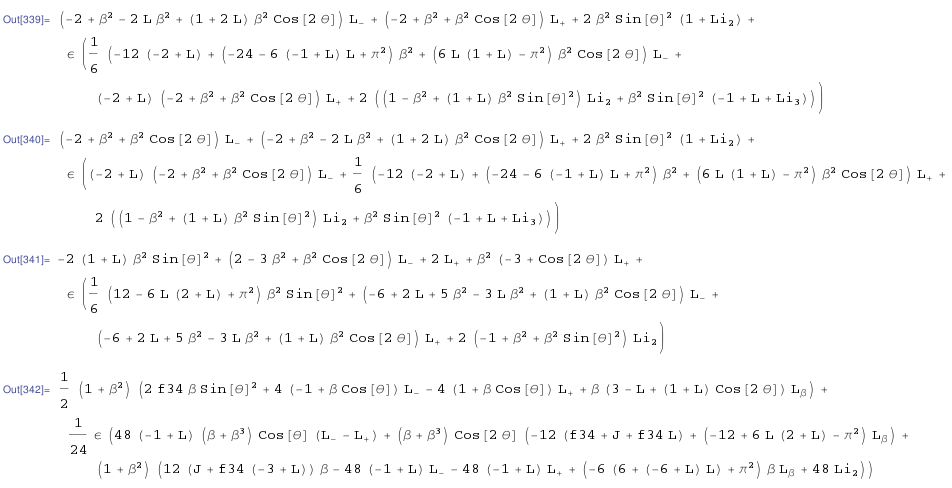
\includegraphics[width=\textwidth]{plots/mixed-soft-function.png}
  \end{center}
  \caption{
   The $C_{jk}$ coefficients of the colour matrices from Eq.~(\ref{eq:
   SMren-res}).
   Notation of Eq.~(\ref{eq:Lplusminu-etc}) expect that $L$ (with no
   subscript) here means $L_\perp$.
  }
  \label{fig:Cjk-coeff}
\end{figure}

%-----------------------------------------------------------------------------
\subsection{Complete $\mathbold{\order{\as^2}}$ mixed contribution }

The NNLO contribution to the differential cross
section~(\ref{eq:factorization-scet}) coming from the mixed term reads
%
\begin{eqnarray}
  \frac{d^4\sigma}{dq_T^2 \, dy \, dM \, d\cos\theta} 
  \bigg |_{\as^2\ \text{mixed}}
  & = &
  \frac{8\pi\beta}{3s M} \frac{1}{2} \int x_Tdx_T \, \, J_0(x_Tq_T) \, \left( \frac{x_T^2M^2}{4e^{-2\gamma_E}} \right)^{-F_{gg}(x_T^2,\mu)}
  \nonumber
  \\
  & & 
  \hspace{40pt} \times \; 4 \frac{3\as^2}{8d_g}\,
  \tr\left[\int \frac{d\phi}{2\pi} [BB\bfH]^{(1)}\bm{W}^{(1)}_{gg} \right]\,,
\end{eqnarray}
%
where the argument of the trace is given in Eq.~(\ref{eq:bbh1wgg1-av}) and we
rewrite here in a slightly different form
%
\begin{eqnarray}
  \int_0^{2\pi} \frac{d\phi}{2\pi}[BB\bfH]^{(1)}\bm{W}^{(1)}_{gg}  & = & 
  %
  \sum_{i,j} \int_{z_1}^{1} \frac{d \xi_1}{\xi_1} 
  \int_{z_2}^{2} \frac{d \xi_2}{\xi_2}
  f_{i/N_1}\left(\frac{z_1}{\xi_1}, \mu\right) 
  f_{j/N_2}\left(\frac{z_2}{\xi_2}, \mu\right)
  %
  \nonumber \\
  & &
  %
  \hspace{-40pt}
  \times \bigg\{
  \frac{1}{4} I_{g\gets i}^{(0)}(\xi_1) I_{g\gets j}^{(0)} (\xi_2)
  \bm{H}^{(1)}_{gg} \bfS_{gg}^{(1)} 
  + \frac{1}{4}
  \Big[
  I_{g\gets i}^{(0)}(\xi_1) \big(I_{g\gets j}^{(1)}(\xi_2) +  
  {I'}_{g\gets j}^{(1)}(\xi_2)\big)
  \nonumber \\
  & &
  + \big(I_{g\gets i}^{(1)}(\xi_1) + 
  {I'}_{g\gets i}^{(1)}(\xi_1) \big) I_{g\gets j}^{(0)}(\xi_2)
  \Big] 
  \bm{H}^{(0)}_{gg}
  \bm{S}^{(1)}_{gg}
  \nonumber 
  \\
  & & 
  \hspace{-20pt}
  + \frac{1}{2 x_T^2}
  \Bigg[
  I_{g\gets i}^{(0)}(\xi_1) {I'}_{g\gets j}^{(1)}(\xi_2)
  +
  {I'}_{g\gets i}^{(1)}(\xi_1) I_{g\gets j}^{(0)}(\xi_2)
  \Bigg]
  \int_0^{2\pi} \frac{d\phi}{2\pi}
  \bm{H}^{M(0)}_{gg}\bm{W}^{(1)}_{gg}
  \bigg\}\,,
  \nonumber \\
  \label{eq:bbh1wgg1-av-rep}
\end{eqnarray}
%
where $I_{g\gets {i}}^{(0)}$ are coefficients which match beam functions into
standard collinear PDFs.

All the quantities are now renormalized.
%
The matching coefficients can be found in~\cite{AntoniaMTh, Becher:2012yn}. The
LO hard function is given by Eq.~(\ref{eq:hard-function-scalar}). The NLO hard
function was computed in~\cite{Ahrens:2011px} and is available in Mathematica
format from the arXiv submission of~\cite{Li:2013mia}.
%
The renormalized average NLO
soft function is given in Eq.~(\ref{eq:soft-function-NLO-ren}) with the colour
matrices collected in Appendix~\ref{app:wmatrices}.
%
Finally the integral from
the last row of the above equation is given in Eq.~(\ref{eq:mixed-integral-av}) with the mixed soft
function given in Eq.~(\ref{eq: SMren-res}) and Fig.~\ref{fig:Cjk-coeff}.



%-----------------------------------------------------------------------------
\chapter{NNLO soft function: general considerations}

\section{Scaling}

Each diagram consists of 


\begin{center}
  {\renewcommand{\arraystretch}{1.0}% for the vertical padding
    \begin{tabular}{cc}
    $d^dk$ & $d$ \\
    $d^dl$ & $d$ \\
    $\delta(k^2)$ & $-2$ \\
    $\delta(l^2)$ & $-2$ \\
    2 $\alpha$ regulators & $-2\alpha$ \\
    transverse delta & $-(d-2)$ \\
    4 quark propagators & $-4$\\
    \hline
    sum: & $d -2 \alpha - 6 = 4-6-2\epsilon - 2\alpha$ \\
         & \hspace{40pt} $= -2 -2\alpha -2\epsilon$
    \end{tabular}
  }
\end{center}

\section{Kinematics}
We need two gluon $d$-vectors
%
\begin{eqnarray}
  k & = & k_{0}\, (1,\ldots,\sin\theta_1\sin\theta_2,
               \sin\theta_1\cos\theta_2,\cos\theta_1)\,, \\
  l & = & l_{0}\, (1,\ldots,\sin\chi_1\sin\chi_2,
               \sin\chi_1\cos\chi_2,\cos\chi_1)\,,
\end{eqnarray}
%
where $\theta_1$ and $\chi_1$ are the polar angles while $\theta_2$ and $\chi_2$
are the azimuthal angles of the gluons.
 
The loop integrals have the form
%
\begin{equation}
  \qquad \qquad \qquad
  \int [dk] [dl]
  \qquad \qquad \qquad \text{where} \qquad  \qquad
  [dk] = d^d k\, \delta(k^2)\, \theta(k^0)\,,
\end{equation}
%
and need to be regularized using the method of Ref.~\cite{Becher:2011dz},
which leads to the replacements
%
\begin{subequations}
   \begin{eqnarray}
     d^d k\, \delta(k^2) \theta(k_0) 
     & \to &
     d^d k \left(\frac{\nu_k}{n \cdot k} \right)^{\alpha}\!
     \delta(k^2)\, \theta(k_0)\,, 
     \\[0.5em]
     d^d l\, \delta(l^2) \theta(l_0) 
     & \to &
     d^d l \left(\frac{\nu_l}{n \cdot l} \right)^{\beta}\!
     \delta(l^2)\, \theta(l_0)\,.
   \end{eqnarray}
   \label{eq:analytic-reg}
\end{subequations}

%-----------------------------------------------------------------------------
\section{Feynman rules for NNLO soft functions}
\label{sec:FRsoft}

In order to understand the Feynman rules we need to remember that the eikonal
vertices come from quark propagators approximated in the soft gluon limit.
%
\begin{itemize}
  \item
  Denominators of the kinetic parts are constructed by going along each quark
  leg $i$ with gluon attachments, assigning momenta as $n_i+k$, $n_i+k+l$ and
  then taking those in eikonal approximation: $n_i \cdot k$, $n_i \cdot (k+l)$,
  etc. 
  %
  Each uncut gluon gets its usual propagator.
  % 
  For example, for the diagram $D_5$ of Fig.~\ref{fig:pecjak2}, that gives $n_i
  \cdot k\, n_i \cdot (k+l)\, n_j \cdot k\, n_j \cdot (k+l)$ while for $D_6$ we
  get $n_i \cdot k\, n_i \cdot (k+l)\, n_j \cdot (k+l) (k+l)^2$.
  \item
  Numerators of the kinetic parts are constructed by simple contractions of
  velocity vectors with corresponding indices.
  %
  \comment{Case of non-abelian diagrams}
  \item
  Colour factors are attributed by starting from the LHS (amplitude) of the cut
  and following gluon attachments along the external lines. 
  %
  Then we move to RHS and follow the lines in the same but put dagger on the
  whole expression, which leads to swapping operators in the final result.
  Three-gluon vertex brings $i f^{abc}$ as usual. Note that the conjugation
  changes the sing of non-abelian amplitudes.
  %
  For example, for diagram $D_5$ of Fig.~\ref{fig:pecjak2} we have 
  $T_i^a T_i^b T_j^b T_j^a$.~\footnote{See my notes for derivation and more
  examples.}
\end{itemize}

%-----------------------------------------------------------------------------
\section{NNLO soft function in position space}

Transformation of the bare NNLO soft function from momentum space to position
space can be schematically written as
%
\begin{align}
  S^{(2)}(L_T) & = 
  \left(f_{-1,0}\, \frac{1}{\epsilon}+ 
  f_{0,1}\, L_T + f_{0,0} + f_{1,2}\, L_T^2\epsilon
  + f_{1,1}\, L_T\epsilon + f_{1,0}\, \epsilon \right)
  \left(s_{-1}\frac{1}{\epsilon} + s_0 + s_1\, \epsilon\right)\,.
\end{align}
%
Hence, the corresponding terms of the position-space soft function read
%
\begin{align}
  S^{(2)}_{-2,0}(L_T) & =  f_{-1,0}\, s_{-1}\, \frac{1}{\epsilon^2}\,,
  \\[0.3em]
  S^{(2)}_{-1,0}(L_T) & =  \left(f_{-1,0}\, s_{0} + f_{0,0}\, s_{-1}\right)\,
                           \frac{1}{\epsilon}\,,
  \\[0.3em]
  S^{(2)}_{-1,1}(L_T) & =  f_{0,1}\, s_{-1} L_T \frac{1}{\epsilon}\,,
  \\[0.3em]
  S^{(2)}_{0,2}(L_T) & =   f_{1,2}\, s_{-1}\, L_T^2\,,
  \\[0.3em]
  S^{(2)}_{0,1}(L_T) & =  \left(f_{0,1}\, s_{0} + f_{1,1}\, s_{-1}\right) L_T\,,
  \\[0.3em]
  S^{(2)}_{0,0}(L_T) & =  \left(f_{-1,0}\, s_{1} + f_{0,0}\, s_{0} +
                                f_{1,0} s_{-1} \right)\,.
  \label{eq:S200}
\end{align}
%
And only the first term in Eq.~(\ref{eq:S200}) needs to be calculated while the
other two can be extracted from RG results for the pole part or for the $L_T$
dependent part.

It is important to note that the finite part of the above object \emph{is not}
equal to the renormalized NNLO soft function one obtains from RG evolution
described in Section~\ref{sec:RGevolution}. The latter includes additional
finite terms coming from pieces like $\tbfS^{(1)}_\bare\bfZ_s^{1}$, as
given in detail in Eq.~(\ref{eq:renS2}).

%-----------------------------------------------------------------------------
\section{Factorization}

Our direct calculation of the bare NNLO soft function and the fact that its pole
structure matches that derived from RGE (real and imaginary part) is a direct
demonstration of small-$q_T$ factorization for this process at this order of
perturbation theory.

%-----------------------------------------------------------------------------
\chapter{NNLO soft function: $\mathbold{n_f}$ part}
%-----------------------------------------------------------------------------

\section{Vacuum polarization integrals}

We consider the process 
%
\begin{equation}
  g(p) \to q(k) + \qbar(p-q)\,.
  %\label{eq:}
\end{equation}

%-----------------------------------------------------------------------------
\subsubsection{Calculation via unitarity}

All propagators are assumed to be defined with $+i\epsilon$ prescription.

\paragraph{Tadpole}
%
The following scalar integral
%
\begin{equation}
  A_0(\alpha_1,\alpha_2) = 
  \int\frac{d^d k}{(n\cdot k)^{\alpha_1}\, (n\cdot (q+k))^{\alpha_2}\, k^2}\,,
  %\label{eq:}
\end{equation}
%
is scaleless and vanishes. To show that, we write
%
\begin{equation}
  %\label{eq:}
  A_0(\alpha_1,\alpha_2)  = 
  \int\frac{d\kp d\km\, k_T^{d-3} dk_T\, d\Omega_{d-3}}
  {k_+^{\alpha_1} (q_++\kp)^{\alpha_2}\, (\kp\km-k_T^2)}\,,
\end{equation}
%
and introduce the rescaling
\begin{equation}
  \km = \lambda\, \km\,, \qquad \qquad
  k_T = \lambda^\frac12\, k_T\,, 
  %\label{eq:}
\end{equation}
%
which leads to
%
\begin{equation}
  %\label{eq:}
  A_0(\alpha_1,\alpha_2)  = 
  \lambda^{1+\frac{d-2}{2}-1} A_0(\alpha_1,\alpha_2)   =
  \lambda^{1-\epsilon} A_0(\alpha_1,\alpha_2)\,. 
\end{equation}

\paragraph{Bubble}

It turns out that the only two-point integral that we need is
%
\begin{equation}
  B_0(\alpha) = 
  \int\frac{d^d k}{(-n\cdot k)^{\alpha}\, (n\cdot (q+k))^{\alpha}\, k^2\,
  (q+k)^2}\,,
  %\label{eq:}
\end{equation}
%
and it can be calculated exactly. After the cut it reads
%
\begin{equation}
  B_0(\alpha) = 
 -2 \pi ^{\frac{d}{2}}\,
  \frac{\Gamma (\epsilon ) \Gamma (1-\alpha -\epsilon )^2 }
  {\Gamma (2-2\alpha -2\epsilon)}\sin (\pi  \epsilon )\,
  q^{-2 \epsilon }\, (n \cdot q)^{-2 \alpha }\,.
  %\label{eq:}
\end{equation}

\paragraph{Vacuum polarization}
%
The self energy tensor has the form
%

\begin{equation}
  \im \Pi^{\mu\nu}(\alpha) = 
  T_{00}\, g^{\mu,\nu} +
  T_{qq}\, q^{\mu}q^{\nu} +
  T_{nn}\, n^{\mu}n^{\nu} +
  T_{qn}\, \left(n^{\mu} q^{\nu}+q^{\mu} n^{\nu}\right)\,
  %\label{eq:}
\end{equation}
%
where
%
\begin{subequations}
  %\label{eq:}
  \begin{align}
  T_{00} &= \frac{2 \left(2 (1-\epsilon)^2-\alpha  (1-2 \epsilon)\right)}
  {(1-\epsilon) (3-2 \alpha -2 \epsilon)}
  \, \calN\, B_0(\alpha)\,
  q^2 
  \,,\\
  %
  T_{qq} &= -\frac{4 (1-\alpha -\epsilon)}{3-2 \alpha -2 \epsilon} 
  \,\calN\, B_0(\alpha)\,,\\
  %
  T_{nn} &= 
  \frac{2 \alpha }{(1-\epsilon) (3-2 \alpha -2 \epsilon)}
  \,\calN\, B_0(\alpha)\,
  \frac{q^4}{\left(n\cdot q\right)^2}
  \,,\\
  %
  T_{qn} &= 
  -\frac{2 \alpha}{(1-\epsilon) (3-2 \alpha -2 \epsilon) }
  \,\calN\, B_0(\alpha)\,
  \frac{q^2}{n\cdot q}
  \,,
  \end{align}
\end{subequations}
%
and
%
\begin{equation}
  \calN = -\frac{g^2}{16} T_F 
  \frac{e^{\epsilon\gamma_E}\mu^{2\epsilon}\nu^{2\alpha}}{\pi^{4-\epsilon}}\,.
  %\label{eq:}
\end{equation}


\section{Soft function integrals}

The above results for the quark bubble can now be embedded into a 2-Wilson-Line
soft function. The integrals have the following general structure
%
\begin{equation}
  I = \int\frac{d^d k\, \delta(k_T^2-1)\, \theta(k^2)\, \theta(k_0)}
      {(n\cdot k)^{a_1+2\alpha} (\nbar\cdot k)^{a_2} (v_3 \cdot k)^{a_3} (v_4
      \cdot k)^{a_4} (k^2)^{a_0+\epsilon}}\,.
  \label{eq:sfnf-general-structure}
\end{equation}
%
What prevents us from direct use of reversed unitarity is the $\theta(k^2)$
function. However, we can trade it for the Dirac delta function at the cost of
introducing extra integration. Namely, we multiply
Eq.~(\ref{eq:sfnf-general-structure}) by 
%
\begin{equation}
  1 = \int_0^\infty dm^2 \delta(k^2-m^2)\,,
  %\label{eq:}
\end{equation}
%
which leads to
\begin{align}
  I & = \int_0^\infty dm^2 \delta(k^2-m^2)
      \int\frac{d^d k\, \delta(k_T^2-1)\, \theta(k^2)\, \theta(k_0)}
      {(n\cdot k)^{a_1+2\alpha} (\nbar\cdot k)^{a_2} (v_3 \cdot k)^{a_3} (v_4
      \cdot k)^{a_4} (k^2)^{a_0+\epsilon}}
    \nonumber \\
    & = \int_0^\infty dm^2 \delta(k^2-m^2)
      \int\frac{d^d k\, \delta(k_T^2-1)\, \theta(m^2)\, \theta(k_0)}
      {(n\cdot k)^{a_1+2\alpha} (\nbar\cdot k)^{a_2} (v_3 \cdot k)^{a_3} (v_4
      \cdot k)^{a_4} (m^2)^{a_0+\epsilon}}
    \nonumber \\
    & = \int_0^\infty dm^2 \frac{\theta(m^2)}{(m^2)^{a_0+\epsilon}}\
      \int\frac{d^d k\, \delta(k_T^2-1)\,\delta(k^2-m^2)  \theta(k_0)}
      {(n\cdot k)^{a_1+2\alpha} (\nbar\cdot k)^{a_2} (v_3 \cdot k)^{a_3} (v_4
      \cdot k)^{a_4}}\,.
  \label{eq:}
\end{align}
%
Hence, we obtain
%
\begin{equation}
  I = \int_0^\infty dm^2 \frac{\theta(m^2)}{(m^2)^{a_0+\epsilon}} \bar I (m^2)\,.
  %\label{eq:}
\end{equation}
%
Now, we can use reversed unitarity to turn delta functions into propagators.
This leads to the following topology
%
\begin{align}
  \label{eq:topology-bubble}
  \bar I(a_1, a_2, a_3, a_4, a_5, a_5)  
  & =   \\ &  \hspace{-30pt}
  \int \frac{d^d k}
  {(n\cdot k)^{a_1+2\alpha} (\nbar\cdot k)^{a_2} (v_3 \cdot k)^{a_3} (v_4
  \cdot k)^{a_4} (k^2-m^2)^{a_5} ((n\cdot k)(\nbar \cdot k)-m^2-1)^{a_6}}\,.
  \nonumber
\end{align}

%-----------------------------------------------------------------------------
\subsection{IBPs}

\begin{enumerate}
  \item
  Standard IBPs:
  \begin{eqnarray}
    \int d^dk\, \frac{\partial}{\partial k^\mu} q^\mu 
    I(a_1,a_2,\ldots, a_{16}) & = & 0\,,
    %\label{eq:}
  \end{eqnarray}
  %
  with $q^\mu = n^\mu, \nbar^\mu, v_3^\mu, v_4^\mu, k^\mu$. This set
  consists of \underline{5 identities}.
  \item
  $q_T$ delta propagator:
  \begin{align}
  I\, \frac{(n\cdot k) (\nbar\cdot k) - m^2-1}
           {(n\cdot k) (\nbar\cdot k) - m^2-1} & = I
  \\[0.5em]
  \text{Ym}[1]\text{Ym}[2]\text{Y}[6] - (m^2+1)\text{Y}[6] & = 1
  \\[0.5em]
  1-\text{Ym}[1]\text{Ym}[2]\text{Y}[6] + (m^2+1)\text{Y}[6] & = 0
  \end{align}
  %
  Hence, we get \underline{1 identity}.
  %
  \item
  Momentum conservation: For $2 \to 3$ kinematics, the exact 4-momenta must
  satisfy
  %
  \begin{equation}
    p_1 + p_2 = p_3 + p_4 + k\,,
    %\label{eq:}
  \end{equation}
  which can be written as
  \begin{equation}
   \frac{M}{2} n + \frac{M}{2} \nbar  = 
   \frac{M}{2} \tilde v_3 + q_3 + \frac{M}{2} \tilde v_4 + q_4 + k\,.
    %\label{eq:}
  \end{equation}
  The above momenta scale as
  %
  \begin{eqnarray}
    n,\, \nbar,\, \tilde v_3,\, \tilde v_4 \sim M (1,1,1)\,, \\
    q_3,\, q_4,\, k \sim M (\lambda, \lambda, \lambda)\,,
    %\label{eq:}
  \end{eqnarray}
  and $q_3$, $q_4$ are constructed such that they balance soft gluon's momentum
  $k$. Hence, $n$, $\nbar$, $\tilde v_3$ and $\tilde v_4$ satisfy the LO, $2\to
  2$ relation
  %
  \begin{equation}
    n + \nbar = \tilde v_3 + \tilde v_4\,.
    %\label{eq:}
  \end{equation}
  Multiplying the above by $k$ leads to the following \underline{1 identity}
  \begin{equation}
    \tilde v_3\cdot k + \tilde v_4\cdot k - n\cdot k  - \nbar\cdot k\,,
    %\label{eq:}
  \end{equation}
  which can be written as
  \begin{equation}
    \text{Ym}[3] + \text{Ym}[4] - \text{Ym}[1] - \text{Ym}[2] = 0\,.
    %\label{eq:}
  \end{equation}
\end{enumerate}

Hence, altogether  we have  7 identities.

%-----------------------------------------------------------------------------
\subsection{Kinematics}
%
Note that the 4-vector $k^\mu$ in Eq.~(\ref{eq:topology-bubble}) is now massive.
Hence, the parametrization from Eq.~(\ref{eq:k4v-par-massless}) does not hold
and it must be replaced with 
%
\begin{equation}
 k  = 
 (k_0, \ldots,
 |\vec k| \sin\theta_1\sin\theta_2, ,|\vec k| \sin\theta_1\cos\theta_2,
 |\vec k| \cos\theta_1)\,,
 \label{eq:k4v-par-massive}
\end{equation}
%
where
%
\begin{equation}
 |\vec k| = \sqrt{k_0^2-m^2}\,.
  %\label{eq:}
\end{equation}
%
Therefore, the relevant inner products now take the form
%
\begin{align}
  n \cdot k & =  k_0 - |\vec k| \cos\theta_1\,, \\
  \nbar \cdot k & =  k_0 + |\vec k| \cos\theta_1\,, \\
  \tilde v_3 \cdot k & =  k_0- 
  \beta\, |\vec k| \sin\theta_1\cos\theta_2\sin\theta -
  \beta\, |\vec k| \cos\theta_1\cos\theta\,, \\
  \tilde v_4 \cdot k & =  k_0+
  \beta\, |\vec k|\sin\theta_1\cos\theta_2\sin\theta +
  \beta\, |\vec k|\cos\theta_1\cos\theta\,.
\end{align}
%
We also get that
%
\begin{align}
 k_0 & = \frac12\left(n\cdot k + \nbar \cdot k\right) \,, \\
 k_0 & = \frac12\left(\tilde v_3\cdot k + \tilde v_4 \cdot k\right)\,.
\end{align}

%-----------------------------------------------------------------------------
\subsection{Derivatives}

\begin{align}
  \frac{d}{d\beta} I & = 
  \left(
  - a_3\, \frac{1}{\tilde v_3 \cdot k}\, \frac{d}{d\beta}(\tilde v_3 \cdot k)  
  - a_4\, \frac{1}{\tilde v_4 \cdot k}\, \frac{d}{d\beta}(\tilde v_4 \cdot k)
  \right)\, I
\end{align}


\begin{align}
  \frac{d}{d\beta}\, \tilde v_3 \cdot k 
  & = 
  - |\vec k| \sin\theta_1\cos\theta_2\sin\theta -
    |\vec k| \cos\theta_1\cos\theta \\
  & = 
  \frac{1}{\beta}\left(\tilde v_3 \cdot k - k_0 \right) \\
  & = 
  \frac{\tilde v_3 \cdot k}{\beta} -
  \frac{n\cdot k}{2\beta} - \frac{\nbar\cdot k}{2\beta} \\
  & = 
  \frac{\tilde v_3 \cdot k}{2\beta} - \frac{\tilde v_4 \cdot k}{2\beta}
\end{align}

\begin{align}
  \frac{d}{d\beta}\, \tilde v_4 \cdot k 
  & = 
    |\vec k| \sin\theta_1\cos\theta_2\sin\theta +
    |\vec k| \cos\theta_1\cos\theta \\
  & = 
  \frac{1}{\beta}\left(\tilde v_4 \cdot k-k_0  \right) \\
  & = 
  \frac{\tilde v_4 \cdot k}{\beta} -
  \frac{n\cdot k}{2\beta} - \frac{\nbar\cdot k}{2\beta} \\
  & = 
  \frac{\tilde v_4 \cdot k}{2\beta} - \frac{\tilde v_3 \cdot k}{2\beta}
\end{align}

The above results allow one to write down the general formula for derivative of
the topology~(\ref{eq:topology-bubble})
%
\begin{equation}
  \frac{d}{d\beta} = 
  -\frac{1}{2\beta}\left\{
  a_3 \left(1-\frac{\tilde v_4 \cdot k}{\tilde v_3 \cdot k}\right) +
  a_4 \left(1-\frac{\tilde v_3 \cdot k}{\tilde v_4 \cdot k}\right)
  \right\}\,.
  %\label{eq:}
\end{equation}


%-----------------------------------------------------------------------------
\chapter{NNLO soft function: real-virtual}

%-----------------------------------------------------------------------------
\section{Soft currents}

Following Ref.~\cite{Bierenbaum:2011gg} we introduce the tree level and (UV-renormalized) one-loop soft currents
%
\begin{align}
  J_a^{\mu (0)} & = \sum_{i=1}^n T_i^a e_i^\mu\,,
  \\
  J_a^{\mu (1)} & = i f^{abc} \sum_{i\neq j=1}^n T_i^b T_j^c 
                    \left(e_i^\mu-e_j^\mu\right) 
		    g_{ij}^{(1)}(\epsilon,q, p_i, p_j)\,,
\end{align}
%
where
%
\begin{equation}
  %\label{eq:}
  e_i^\mu = \frac{p_i^\mu}{p_i \cdot q}\,,
\end{equation}
%
and the function $g_{ij}$ is symmetric under the exchange $i\leftrightarrow j$.

%-----------------------------------------------------------------------------
\section{Diagrams of the type 123}

\begin{figure}[t]
  \begin{center}
    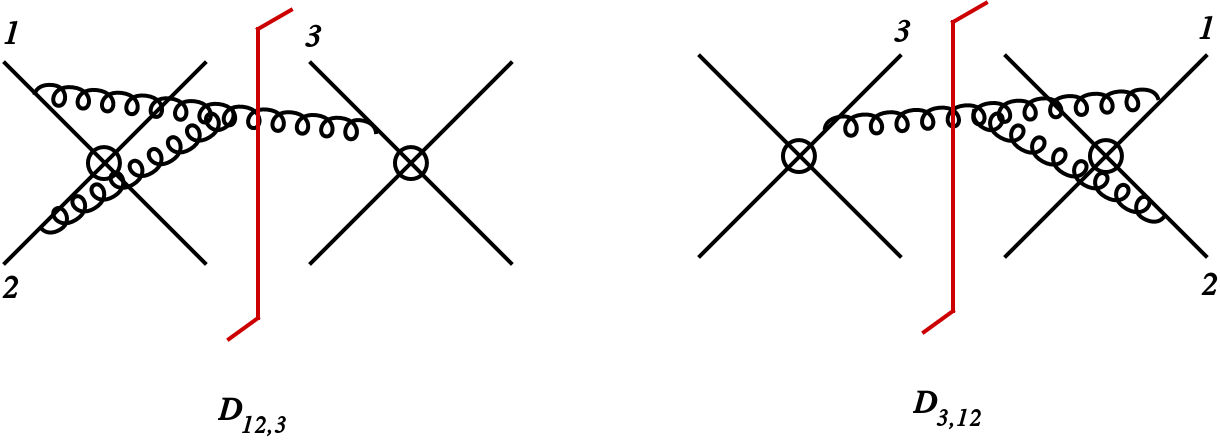
\includegraphics[width=0.80\textwidth]{plots/sf-nnlo-1cut123.png}
  \end{center}
  \caption{
  }
  \label{fig:diag123}
\end{figure}

Let us consider a special case of 3-Wilson-line diagrams which involve two
massless and one massive particle. Two such diagrams are depicted in
Fig.~\ref{fig:diag123}.

Using the notation introduced above we can write expressions corresponding to
those two diagrams
%
\begin{align}
  D_{12,3} & = i f^{abc}\, T_3^a T_1^b T_2^c\, 
             \left(e_1^\mu-e_2^\mu\right) e_3^\mu\, g_{12}^{(1)}\,,
  \\[0.5em]
  D_{3,12} & = -i f^{abc}\, T_3^a T_1^b T_2^c\, 
             \left(e_1^\mu-e_2^\mu\right) e_3^\mu\, g_{12}^{(1)\,*}\,.
\end{align}
%
Hence, their sum reads
%
\begin{equation}
  D_{12,3}  + D_{3,12}  = i f^{abc}\, T_3^a T_1^b T_2^c\, 
                          \left(e_1^\mu-e_2^\mu\right) e_3^\mu\,
	                  \left(g_{12}^{(1)}-g_{12}^{(1)\,*}\right)\,.
  %\label{eq:}
\end{equation}

We see that the result is purely imaginary and that it does not vanish as the
antisymmetry of the colour factor under the exchange $1 \leftrightarrow 2$ is
compensated by the antisymmetry of the kinematic part.

This is in contradiction with the claims made in Ref.~\cite{Becher:2009qa} where
it is argued that all three-particle structures with two massless and one
massive Wilson lines must vanish. This conclusion, however, follows from the
constraint imposed on the form of the anomalous dimension which is a consequence
of factorization. Yet, the latter is not proven anywhere in the discussion but
it is only assumed.

%------------------------------------
\subsection*{Scaling}

The soft current for massless particles with momenta $p_{1,2} = (1,0,0,\pm 1)$
reads~\cite{Catani:2000pi}
%
\begin{align}
  J_{2P}^{a(1)}(p_1,p_2;q, \epsilon) & = 
  -\frac{1}{16\pi^2}  i f_{abc} T_1^b T_2^c\, \epsilon_\mu(q)
  \left(\frac{p_1^\mu}{p_1\cdot q}- \frac{p_2^\mu}{p_2\cdot q}\right)
  \nonumber \\
  & \times
  \left(\frac{4\pi p_1\cdot p_2}{2 p_1 \cdot q\, p_2 \cdot q e^{-i\pi}}
  \right)^\epsilon
  \frac{1}{\epsilon^2}
  \frac{\Gamma^3(1-\epsilon)\Gamma^2(1+\epsilon)}{\Gamma(1-2\epsilon)}\,.
\end{align}
%
Embedding the above in the integral over $q$ gives
%
\begin{align}
  G_{12,3} & \propto i f_{abc} T_3^a T_1^b T_2^c\,
  \frac{1}{\epsilon^2}\,
  \frac{\Gamma^3(1-\epsilon)\Gamma^2(1+\epsilon)}{\Gamma(1-2\epsilon)}
  \nonumber \\
  & \times
  \int d^d q\,
  \frac{\delta^+(q^2)\delta^{(2)}(q_\perp-1)}
       {q_+ p_{3-}+q_- p_{3+}-q_\perp \cdot p_{3\perp}}\,
  \frac{1}{q_+^\alpha}
  \left(\frac{p_{3+}}{q_+}- \frac{p_{3-}}{q_-}\right)
  \left(\frac{4\pi}{q_+\, q_-\, e^{-i\pi}}
  \right)^\epsilon.
\end{align}
%
Let us now apply the change of variables, motivated by Ref.~\cite{Aybat:2006wq}
%
\begin{equation}
  (q_+,q_-,q_\perp) \to (\xi q_-,\xi^{-1} q_+,q_\perp)
  \qquad
  \text{with} 
  \quad
  \xi = p_{3+}/p_{3-}\,.
  \quad
  %\label{eq:}
\end{equation}
%
Our integral becomes
%
\begin{align}
  G_{12,3} (\alpha) & \propto i f_{abc}  T_3^a T_1^b T_2^c \,
  \frac{1}{\epsilon^2}\,
  \frac{\Gamma^3(1-\epsilon)\Gamma^2(1+\epsilon)}{\Gamma(1-2\epsilon)}
  \nonumber \\
  & \times
  \int d^d q\, 
  \frac{\delta^+(q^2)\delta^{(2)}(q_\perp-1)}
       {q_+ p_{3-}+q_- p_{3+}-q_\perp \cdot
  p_{3\perp}}
  \xi^{-\alpha}\frac{1}{q_-^\alpha}
  \left(\frac{p_{3-}}{q_-} - \frac{p_{3+}}{q_+}\right)
  \left(\frac{4\pi}{q_+\, q_-\, e^{-i\pi}}
  \right)^\epsilon
  \nonumber \\
  & = - \xi^{-\alpha} G_{12,3}(-\alpha)\,.
\end{align}
%
Hence, we see that the above integral would exhibit scaling and vanish if only
there was no $\alpha$ regulator. However, without the regulator, the integral is
divergent. Hence, we conclude that the tree-particle graph with two massless and
one massive Wilson lines does not vanish.

A few comments are in order:
%
\begin{enumerate}
  \item
  The above result will only affect the imaginary part of the soft function. The
  tree-particle graphs of the type of 123 will not contribute to the soft
  function as there will always be a complex-conjugate diagram with opposite
  sign due to colour operator.
  \item
  The above result does not invalidate the analysis of Ref.~\cite{Aybat:2006wq},
  where it is claimed that the massless-massless-massive diagrams vanish because
  of certain scaling properties. The key difference between our case and the one
  discussed there is that in Ref.~\cite{Aybat:2006wq} purely virtual diagrams
  are consider. And in those diagrams, rapidity divergences are regularized by
  dimensional regularization~\cite{Becher:2011dz}.  Hence, no $\alpha$ regulator
  is required and the scaling holds.
  \item
  The key element of our calculation, which prevents the diagram 123 from
  vanishing, is the transverse delta function. As explained in
  Ref.~\cite{Becher:2011dz} without this function, integration over the
  transverse momentum provides a factor $k_-^{-\epsilon}$ which regularizes
  rapidity divergences. However, when the transverse delta is present it fixes
  $q_\perp$ to some external value and the integration of $q_\perp$ does
  provide a regular of light-cone singularities. Hence, we need to introduce
  $\alpha$.
\end{enumerate}

%-----------------------------------------------------------------------------
\chapter{NNLO soft function: double real}
\section{Double-real NNLO integrals}

At NNLO, we have two gluons which connect the Wilson lines in various ways.
Ref.~\cite{Ferroglia:2012uy} distinguishes the following types of integrals: 
%
\begin{itemize}
  \item
   \emph{two-Wilson-line integrals}: two gluons connect only two types
   of Wilson lines $i$ and $j$,
  \item
   \emph{three-Wilson-line integrals}: two gluons connect three types
   of Wilson lines $i$, $j$ and $k$,
  \item
   \emph{four-Wilson-line integrals}: two gluons connect four types of
   Wilson lines $i$, $j$, $k$ and $l$.
\end{itemize}

The relevant integrals can be deduced from Ref.~\cite{Ferroglia:2012uy}, where,
however, fully massless case in the threshold limit is considered. Our \ttbar
production requires the following modifications of the original formulae:
%
\begin{itemize}
  \item
  The delta functions get the replacement:
  $\delta(\omega - n_0 \cdot (k+l)) \to \delta^{(2)}(q_\perp-k_\perp-l_\perp)$,
  which comes from replacing the threshold limit by the soft limit.
  \item
  Integrals are regularized according to Eqs.~(\ref{eq:analytic-reg}).
\end{itemize}

In the following subsections, we shall present the formulae for two-, three- and
four-Wilson-line integrals. For better readability, we will skip the common
factor
%
\begin{equation}
  \Sigma' = v_k^\alpha v_l^\beta\,,
  %\label{eq:}
\end{equation}
%
which shall be restored at the end of the calculation.~\footnote{The above needs
to be adjusted further with $\msbar$ related factors etc.}

%-----------------------------------------------------------------------------
\subsubsection{Two-Wilson-line integrals}

\begin{figure}[t]
  \begin{center}
    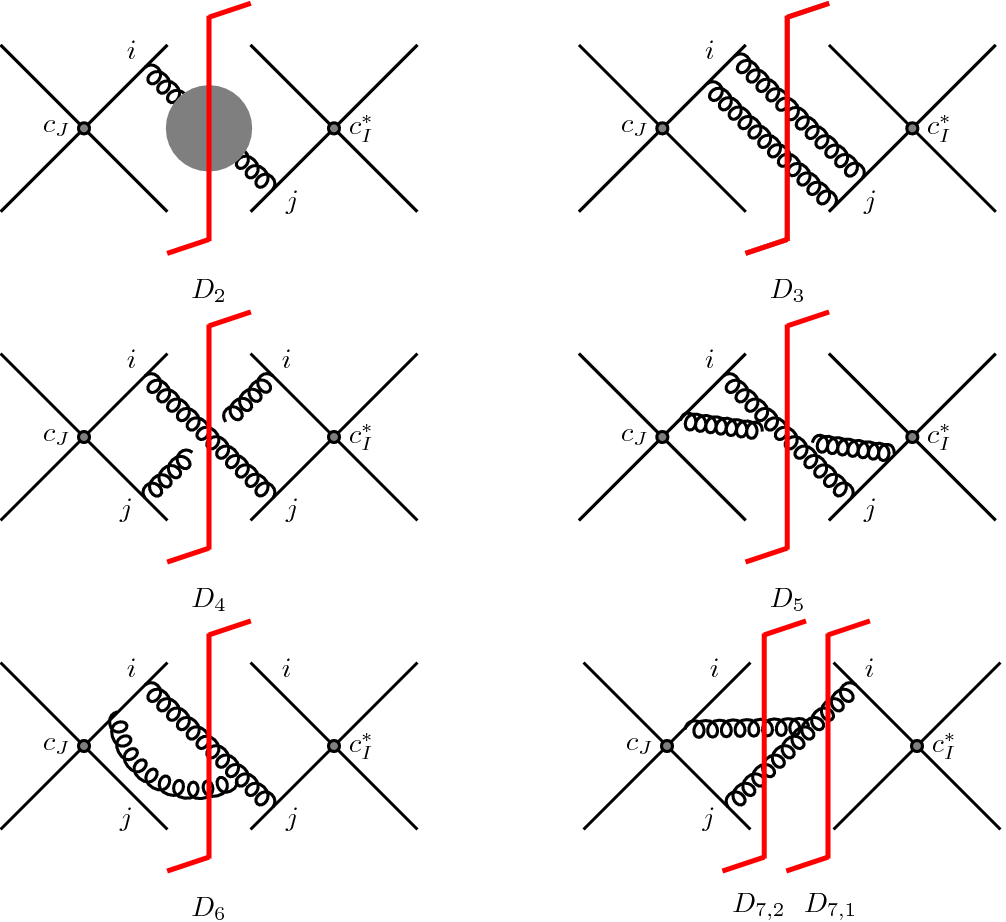
\includegraphics[width=0.7\textwidth]{plots/diagram2-pecjak.png}
  \end{center}
  \caption{Two-Wilson-line integrals for the soft function in the massless case.
  Figure from~\cite{Ferroglia:2012uy}. Our expressions for \ttbar production
  correspond to diagrams with the gluons attached to both initial
  (massless) and final (massive) Wilson lines.}
  \label{fig:pecjak2}
\end{figure}

The relevant integrals correspond to diagrams of Fig.~\ref{fig:pecjak2}, taken
from Ref. ~\cite{Ferroglia:2012uy}. 
%
The expressions read
%
\begin{subequations}
  \label{eq:2WLIset}
  \begin{align}
    %%%
    I_{3, ij} &= 
    (n_i \cdot n_j)^2
    \int d^d k\, d^d l\; 
    \frac{\delta_+(k^2) \, \delta_+(l^2)\,
      \; \delta^{(2)}(q_\perp-k_\perp-l_\perp)}
      {(n \cdot k)^\alpha\; (n \cdot l)^\beta \; 
      n_i \cdot k \; n_i \cdot
      (k+l) \; n_j \cdot l \; n_j \cdot (k+l)} \, ,
    \\[0.7em]
    %%%
    I_{4, ij} &= 
    (n_i \cdot n_j)^2
    \int d^d k\, d^d l\; 
    \frac{\delta_+(k^2) \, \delta_+(l^2) \,
      \; \delta^{(2)}(q_\perp-k_\perp-l_\perp)}
      {(n \cdot k)^\alpha\; (n \cdot l)^\beta \;
      n_i \cdot k \; n_i \cdot l \;
      n_j \cdot k \; n_j \cdot l} \, ,
    \\[0.7em]
    %%%
    I_{5, ij} &=
    (n_i \cdot n_j)^2
    \int d^d k\, d^d l\; 
    \frac{\delta_+(k^2) \, \delta_+(l^2) \,
      \; \delta^{(2)}(q_\perp-k_\perp-l_\perp)}
      {(n \cdot k)^\alpha\; (n \cdot l)^\beta  \;
      n_i \cdot k \; n_i \cdot
      (k+l) \; n_j \cdot k \; n_j \cdot (k+l)} \, , 
    \\[0.7em]
    %%%
    \label{eq:I6ij}
    I_{6,ij} &=
    n_i \cdot n_j
    \int d^d k\, d^d l\; 
    \frac{n_i \cdot (l-k) \;\delta_+(k^2) \, \delta_+(l^2) \, 
     \delta^{(2)}(q_\perp-k_\perp-l_\perp)}
      {(n \cdot k)^\alpha\; (n \cdot l)^\beta  \;
      n_i \cdot k \; n_i \cdot (k+l) \; n_j \cdot (k+l) \; (k+l)^2} \, , 
    \\[0.7em]
    %%%
    \label{eq:I72ij}
    I_{7,2, ij} &=
    n_i \cdot n_j
    \int d^d k\, d^d l\; 
    \frac{n_j \cdot (k+2l) \; \delta_+(k^2) \, \delta_+(l^2) \,
      \delta^{(2)}(q_\perp-k_\perp-l_\perp)}
      {(n \cdot k)^\alpha\; (n \cdot l)^\beta  \;
      n_i \cdot k \; n_j \cdot (k+l) \; n_j \cdot l \; (k+l)^2} \, .
  \end{align}
\end{subequations}
%
where
\begin{equation}
  n_1 = n,     \qquad \qquad
  n_2 = \nbar, \qquad \qquad
  n_3 = \tilde v_3,   \qquad \qquad
  n_4 = \tilde v_4\,.
  \label{eq:nnlo-external-particles}
\end{equation}
%
We note that the above integrals are invariant under rescaling of external
momenta. This will be also true for three- and four-Wilson-line integrals.
Hence, we can work with $v_{3,4}$ or $\tilde v_{3,4}$. We choose the latter as
it leads to more compact expressions.
 
For the time being, we put aside $I_{2, ij}$ and 
$I_{7,1, ij}$ as they are effectively expressible in terms of 1-loop integrals.
These cases will be discussed in next section.

In the massless case, all diagonal terms vanish, as they are proportional to
$n_i^2 = 0$. (This originates from the use of dimensional regularization in
which scaleless integrals are zero.) In \ttbar production, this is certainly true
for the incoming particles, hence for $i=1,2$, whereas the other two diagonal
integrals with $i=3,4$ are in general non-zero.~\footnote{
There are certainly other symmetries between those integrals, which we can
study later.
%
In particular, there is a chance that, since we adopted the analytic regularization scheme
of~\cite{Li:2013mia}, the integrals $I_{12}$ and $I_{21}$ are also
scaleless and vanish as well~(see~\cite{Becher:2010tm}). 
%
This was true at NLO but here would need to be checked directly. For the time
being, we assume that those integrals do not vanish.
%
BTW, the integrals $I_{12}$ and $I_{21}$
do not vanish in the threshold limit~\cite{Ahrens:2010zv}, where the delta
function breaks scalelessness, or in the soft limit with a different
regularization scheme, as
in~\cite{Chiu:2012ir}. Both of the above calculations render non-vanishing
soft functions with non-diagonal initial-initial connections. 
%
As mentioned in~\cite{Li:2013mia}, vanishing of  $I_{12 (21)}$ integrals in
certain scheme does not break scheme-independence as those integrals can be
absorbed into collinear sectors~\cite{Li:2013mia}, hence disappear, in any
scheme.
}
%
More specifically, the five sets of integrals given in Eqs.~(\ref{eq:2WLIset})
have the following structure
%
\begin{subequations}
  \begin{align}
    I_{3, ij},\ I_{5, ij},\ I_{6, ij} &= 
    \left(
    \begin{array}{cccc}
    0      & I_{12} & I_{13} & I_{14} \\
    I_{21} & 0      & I_{23} & I_{24} \\
    I_{31} & I_{32} & I_{33} & I_{34} \\
    I_{41} & I_{42} & I_{43} & I_{44} 
    \end{array}
    \right)\,,
    \\[0.7em]
    %%%
    I_{4, ij},\ I_{7,2, ij} &= 
    \left(
    \begin{array}{cccc}
    0      & I_{12} & I_{13} & I_{14} \\
    I_{21} & 0      & I_{23} & I_{24} \\
    I_{31} & I_{32} & 0      & I_{34} \\
    I_{41} & I_{42} & I_{43} & 0 
    \end{array}
    \right)\,.
  \end{align}
  %\label{eq:}
\end{subequations}
 
Vanishing of $I_{11}$ and $I_{22}$ has been explained above. The reason why there
are no $I_{33}$ and $I_{44}$ integrals in the second matrix is clear by looking
at the corresponding diagrams in Fig.~\ref{fig:pecjak2}. 

Setting $i=j$ in $D_4$ or $D_{7,2}$ would turn them into $D_5$ and $D_6$,
respectively. But the corresponding expressions from Eqs.~(\ref{eq:2WLIset})
would be wrong since, \eg $D_4$ corresponds to a product of four different
Wilson lines, expanded to order $g_s$, whereas $D_5$ represents two Wilson
lines, each expanded to order $g_s^2$. So, the diagonal expressions for
$I_{4, ij}$ and $I_{7,2, ij}$ simply make no sense and should not be calculated.
%
Another way to see this is by noticing that $D_4$ is in fact a convolution of
two NLO soft functions as none of the momenta attaches to the same
line twice.



%-----------------------------------------------------------------------------
\subsubsection{Three-Wilson-line integrals}


From Fig.~\ref{fig:pecjak3} and the Feynman rules of sec.~\ref{sec:FRsoft} we
deduce the following integrals~\cite{Ferroglia:2012uy} 
%
\begin{subequations}
  \label{eq:3WLIset}
  \begin{align}
    %%%
    I_{8, ijk}^{(a)+(b)} &= 
    n_i \cdot n_j\; n_i \cdot n_k\; 
    \int d^d k\, d^d l\; 
    \frac{\delta_+(k^2) \, \delta_+(l^2)\,
      \; \delta^{(2)}(q_\perp-k_\perp-l_\perp)}
      {(n \cdot k)^\alpha\; (n \cdot l)^\beta \; 
      n_i \cdot k \; n_i \cdot l \; n_j \cdot k \; n_k \cdot l} \, ,
    \\[0.7em]
    %%%
    I_{8, ijk}^{(c)+(d)} &= 
    n_i \cdot n_j\; n_i \cdot n_k\; 
    \int d^d k\, d^d l\; 
    \frac{\delta_+(k^2) \, \delta_+(l^2)\,
      \; \delta^{(2)}(q_\perp-k_\perp-l_\perp)}
      {(n \cdot k)^\alpha\; (n \cdot l)^\beta \; 
      n_i \cdot l \; n_i \cdot (k+l) \; n_j \cdot k \; n_k \cdot l} \, ,
    \\[0.7em]
    %%%
    I_{8, ijk}^{(e)+(f)} &= 
    n_i \cdot n_j\; n_i \cdot n_k\; 
    \int d^d k\, d^d l\; 
    \frac{\delta_+(k^2) \, \delta_+(l^2)\,
      \; \delta^{(2)}(q_\perp-k_\perp-l_\perp)}
      {(n \cdot k)^\alpha\; (n \cdot l)^\beta \; 
      n_i \cdot k \; n_i \cdot (k+l) \; n_j \cdot k \; n_k \cdot l} \,,
  \end{align}
\end{subequations}
%
and the external particles are defined as in
Eq.~(\ref{eq:nnlo-external-particles}).
%
Each of the above integrals is proportional to a different colour factor.

\begin{figure}[t]
  \begin{center}
    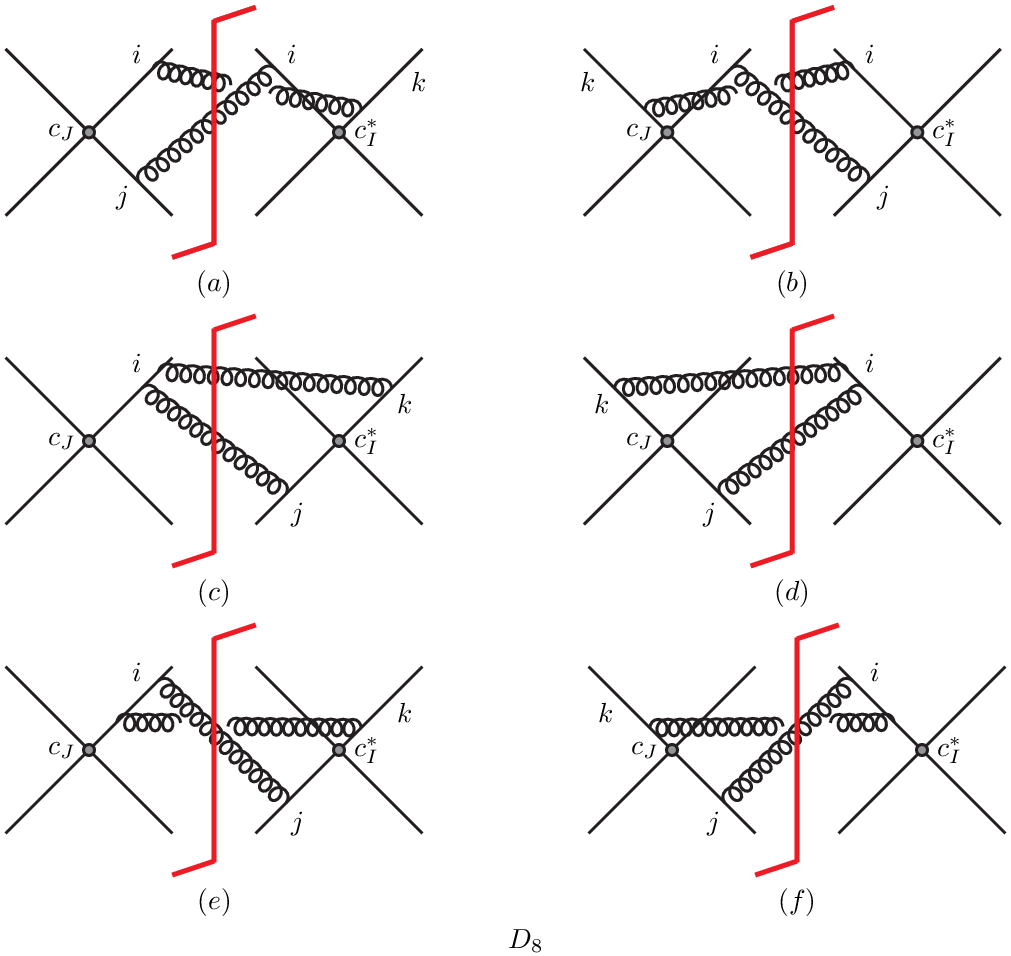
\includegraphics[width=0.7\textwidth]{plots/diagram3-pecjak.png}
  \end{center}
  \caption{
    Three-Wilson-line integrals, the abelian case.
  }
  \label{fig:pecjak3}
\end{figure}
%
\begin{figure}[t]
  \begin{center}
    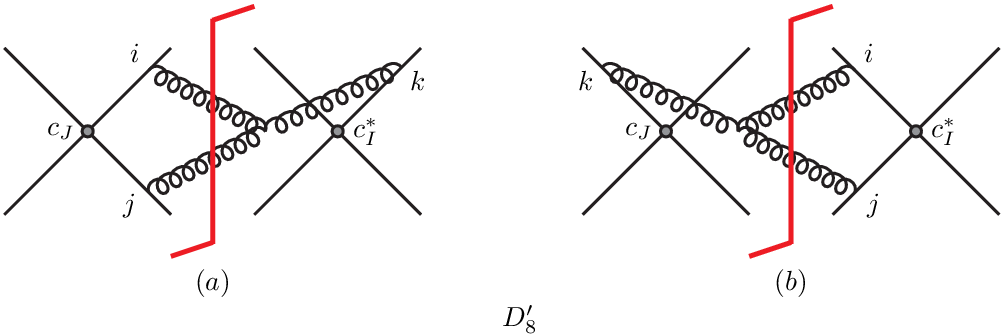
\includegraphics[width=0.7\textwidth]{plots/diagram5-pecjak.png}
  \end{center}
  \caption{
    Three-Wilson-line integrals, the non-abelian case.
  }
  \label{fig:pecjak5}
\end{figure}

Diagrams $(a)$ and $(b)$ are again convolutions of NLO soft functions, hence we
set all the diagonal terms: $I_{iik}, I_{iji}, I_{ijj}$ to zero. 
%
As for $(c), (d), (e)$ and $(f)$, we may have $I_{iik}, I_{iji}$ but not
$I_{ijj}$, as the latter would involve only two Wilson lines. Of the first two,
the integrals do not vanish only if $i=3,4$. In summary, the three-Wilson-lines
integrals given in Eqs.~(\ref{eq:3WLIset}) and represented by diagrams in
Fig.~\ref{fig:pecjak3} are non-vanishing except for
%
\begin{equation}
  \begin{array}{ccc}
  I^{(a,b)}_{8,ijk} = 0     & \quad \text{if} \quad & 
                               i=j\ \lor\ i=k\ \lor\ j=k\,,
  \\[0.5em]
  I^{(c,d,e,f)}_{8,ijk} = 0 & \quad \text{if} \quad & j=k\,,
  \\[0.5em]
  I^{(c,d,e,f)}_{8,ijk} = 0 & \quad \text{if} \quad & 
                              (i=j\ \lor\ i=k)\ \land\ (i=1\ \lor\ i=2)\,.
  \end{array}
  %\label{eq:}
\end{equation}

There is also a group of non-abelian integrals like those shown in
Fig.~\ref{fig:pecjak5}. The sum of those two diagrams vanishes due to colour
structure as, following the Feynman rules discussed earlier, we have
%
\begin{subequations}
  \begin{align}
   D'^{(a)}_8 &\propto i f^{abc}\, T_i^a\, T_j^b\, T_k^c\, I'_8\,, \\
   D'^{(b)}_8 &\propto -i f^{abc}\, T_i^a\, T_j^b\, T_k^c\, I'_8\,.
  \end{align}
  %\label{eq:}
\end{subequations}
%
The relative minus sign comes from the fact that the gluon propagator carrying
momentum $k+l$ appears on opposite sides of the cut in the two diagrams
(see sec.~3.2 in ~\cite{Ferroglia:2012uy} for further discussion).
%
The same is true for one-particle cut diagrams analogous to those of
Fig.~\ref{fig:pecjak5}.



%-----------------------------------------------------------------------------
\subsubsection{Four-Wilson-line integrals}
 
\begin{figure}[t]
  \begin{center}
    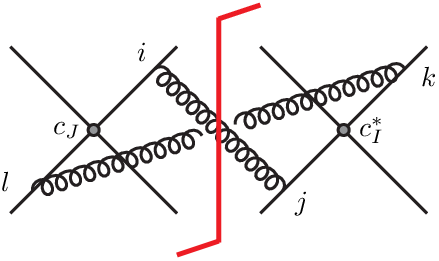
\includegraphics[width=0.35\textwidth]{plots/diagram6-pecjak.png}
  \end{center}
  \caption{
    Four-Wilson-line integrals.
  }
  \label{fig:pecjak6}
\end{figure}

Finally, we have the integrals corresponding to Fig.~\ref{fig:pecjak6}, with 
four different gluon attachments~\cite{Ferroglia:2012uy}
%
\begin{align}
  %%%
  \label{eq:4WLIset}
  I_{9, ijkl} &= 
  n_i \cdot n_j\; n_k \cdot n_l\; 
  \int d^d k\, d^d l\; 
  \frac{\delta_+(k^2) \, \delta_+(l^2)\,
    \; \delta^{(2)}(q_\perp-k_\perp-l_\perp)}
    {(n \cdot k)^\alpha\; (n \cdot l)^\beta \; 
    n_i \cdot k \; n_j \cdot k \; n_k \cdot l \; n_l \cdot l} \,.
\end{align}

Some of the indices have a chance to be equal and render the integral non-zero
provided that the gluons are attached to four distinct Wilson lines and, as
usual, only the squares of massive vectors, hence $n_i^2$ with $i=3,4$, survive.
On the other hand, if the two indices on the same side of the cut become equal,
that corresponds to three-Wilson-lines diagram and should be rejected.
We can summarize the above by
%
\begin{equation}
  \begin{array}{ccc}
  I_{9, ijkl} = 0  &\quad \text{if} \quad & (i=j\ \land\ i = 1,2)\ \lor\
                                            (k=l\ \land\ k = 1,2)\,,
  \\[0.5em]
  I_{9, ijkl} = 0  &\quad \text{if} \quad & i=l\ \lor\ k=j\,.
  \end{array}
  %\label{eq:}
\end{equation}

%------------------------------------
\section{General form of NNLO integral}

We would like to write all the above cases of two-, three- and four-Wilson-line
integrals, given in Eqs.~(\ref{eq:2WLIset}), (\ref{eq:3WLIset})
and~(\ref{eq:4WLIset}), as a single topology. 
%
Because of the argument of the $\delta^{(2)}(q_\perp-k_\perp-l_\perp)$ function,
it is useful to change variables according to
%
\begin{subequations}
\begin{align}
  k &= k\,,  \\
  p &= k+l \quad \to \quad l = p-k\,, 
  \label{eq:p-def}
\end{align}
\end{subequations}
%
which, similarly to the NLO case, allows one to write
%
\begin{equation}
  \delta^{(2)}(q_\perp-k_\perp-l_\perp) = 2 \delta(p_T^2-q_T^2) \delta(\phi)\,,
  %\label{eq:}
\end{equation}
%
where $\phi$ is the azimuthal angle of $p_\perp$ and the azimuthal integral
can be performed trivially.

Then, we notice that $I_{6,ij}$ and $I_{7,2,ij}$, given in Eqs.~(\ref{eq:I6ij})
and~(\ref{eq:I72ij}), can be split such that
%
\begin{eqnarray}
  I_{6,ij} & = & I^{(a)}_{6,ij} - 2 I^{(b)}_{6,ij}\,, \\
  I_{7,2,ij} & = &  I^{(a)}_{7,2,ij} + I^{(b)}_{7,2,ij}\,,
  %\label{eq:}
\end{eqnarray}
%
with the integrals on the RHS involving only three denominators and no
propagator in the numerator.

The full set of integrals which need to be calculated reads 
%
\begin{subequations}
  \label{eq:fullset}
  \begin{align}
    %%%
    I_{3, ij} &= 
    (n_i \cdot n_j)^2
    \int 
    \frac{d^d k\, d^d p\;\delta_+(k^2)\, \delta_+((p-k)^2)\,\delta(p_T^2-q_T^2)}
      {(n \cdot k)^\alpha\; (n \cdot [p-k])^\beta \; 
      (n_i \cdot k) \; (n_i \cdot p) \; (n_j \cdot [p-k]) \; (n_j \cdot p)} \, ,
    \\[0.7em]
    %%%
    I_{4, ij} &= 
    (n_i \cdot n_j)^2
    \int 
    \frac{d^d k\, d^d p\;\delta_+(k^2)\, \delta_+((p-k)^2)\,\delta(p_T^2-q_T^2)}
      {(n \cdot k)^\alpha\; (n \cdot [p-k])^\beta \;
      (n_i \cdot k) \; (n_i \cdot [p-k]) \;
      (n_j \cdot k) \; (n_j \cdot [p-k])} \, ,
    \\[0.7em]
    %%%
    I_{5, ij} &=
    (n_i \cdot n_j)^2
    \int 
    \frac{d^d k\, d^d p\;\delta_+(k^2)\, \delta_+((p-k)^2)\,\delta(p_T^2-q_T^2)}
      {(n \cdot k)^\alpha\; (n \cdot [p-k])^\beta  \;
      (n_i \cdot k) \; (n_i \cdot p) \; 
      (n_j \cdot k) \; (n_j \cdot p)} \, , 
    \\[0.7em]
    %%%
    I^{(a)}_{6,ij} &=
    n_i \cdot n_j
     \int 
    \frac{d^d k\, d^d p\;\delta_+(k^2)\, \delta_+((p-k)^2)\,\delta(p_T^2-q_T^2)}
      {(n \cdot k)^\alpha\; (n \cdot [p-k])^\beta  \;
      (n_i \cdot k) \; (n_j \cdot p) \; p^2} \, , 
    \\[0.7em]
    %%%
    I^{(b)}_{6,ij} &=
    n_i \cdot n_j
    \int 
    \frac{d^d k\, d^d p\;\delta_+(k^2)\, \delta_+((p-k)^2)\,\delta(p_T^2-q_T^2)}
      {(n \cdot k)^\alpha\; (n \cdot [p-k])^\beta  \;
      (n_i \cdot p) \; (n_j \cdot p) \; p^2} \, , 
    \\[0.7em]
    %%%
    I^{(a)}_{7,2, ij} &=
    n_i \cdot n_j
    \int 
    \frac{d^d k\, d^d p\;\delta_+(k^2)\, \delta_+((p-k)^2)\,\delta(p_T^2-q_T^2)}
      {(n \cdot k)^\alpha\; (n \cdot [p-k])^\beta  \;
      (n_i \cdot k) \;  (n_j \cdot [p-k]) \; p^2} \, ,
    \\[0.7em]
    %%%
    I^{(b)}_{7,2, ij} &=
    n_i \cdot n_j
    \int 
    \frac{d^d k\, d^d p\;\delta_+(k^2)\, \delta_+((p-k)^2)\,\delta(p_T^2-q_T^2)}
      {(n \cdot k)^\alpha\; (n \cdot [p-k])^\beta  \;
      (n_i \cdot k) \; (n_j \cdot p) \; p^2} = I^{(a)}_{6,ij}\, ,
    \\[0.7em]
    %%%
    I_{8, ijk}^{(a)+(b)} &= 
    n_i \cdot n_j\; n_i \cdot n_k\; 
    \int 
    \frac{d^d k\, d^d p\;\delta_+(k^2)\, \delta_+((p-k)^2)\,\delta(p_T^2-q_T^2)}
      {(n \cdot k)^\alpha\; (n \cdot [p-k])^\beta \; 
      (n_i \cdot k) \; (n_i \cdot [p-k]) \; 
      (n_j \cdot k) \; (n_k \cdot [p-k])} \, ,
    \\[0.7em]
    %%%
    I_{8, ijk}^{(c)+(d)} &= 
    n_i \cdot n_j\; n_i \cdot n_k\; 
    \int 
    \frac{d^d k\, d^d p\;\delta_+(k^2)\, \delta_+((p-k)^2)\,\delta(p_T^2-q_T^2)}
      {(n \cdot k)^\alpha\; (n \cdot [p-k])^\beta \; 
      (n_i \cdot [p-k]) \; (n_i \cdot p) \; 
      (n_j \cdot k) \; (n_k \cdot [p-k])} \, ,
    \\[0.7em]
    %%%
    I_{8, ijk}^{(e)+(f)} &= 
    n_i \cdot n_j\; n_i \cdot n_k\; 
    \int 
    \frac{d^d k\, d^d p\;\delta_+(k^2)\, \delta_+((p-k)^2)\,\delta(p_T^2-q_T^2)}
      {(n \cdot k)^\alpha\; (n \cdot [p-k])^\beta \; 
      (n_i \cdot k) \; (n_i \cdot p) \; (n_j \cdot k) \; (n_k \cdot [p-k])} \,,
    \\[0.7em]
    %%%
    I_{9, ijkl} &= 
    n_i \cdot n_j\; n_k \cdot n_l\; 
    \int 
    \frac{d^d k\, d^d p\;\delta_+(k^2)\, \delta_+((p-k)^2)\,\delta(p_T^2-q_T^2)}
      {(n \cdot k)^\alpha\; (n \cdot [p-k])^\beta \; 
      (n_i \cdot k) \; (n_j \cdot k) \; (n_k \cdot [p-k]) \; 
      (n_l \cdot [p-k])} \, ,
  \end{align}
\end{subequations}
%
where we skipped the overall numerical factor of
$\Sigma''= 2 v_k^\alpha v_l^\beta$.

Now the argument of the last delta function has to be expressed in terms of
existing propagators. Unlike in the NLO case, here, the 4-vector $p$ is massive
%
\begin{equation}
 p  = (p_0, \ldots,|\vec p| \sin\phi_1\sin\phi_2, ,|\vec p| \sin\phi_1\cos\phi_2,
                   |\vec p| \cos\phi_1)\,,
  %\label{eq:}
\end{equation}
%
hence
%
\begin{equation}
  p^2 =  p_0^2 - p_T^2 - |\vec p|^2 \cos^2\phi_1\,
  %\label{eq:}
\end{equation}
%
which, using Eq.~(\ref{eq:nnbar-defs}) gives
%
\begin{equation}
  p^2 = (n\cdot p) (\nbar \cdot p) -p_T^2.
  %\label{eq:}
\end{equation}
%
Thus
%
\begin{equation}
  \delta(p_T^2 - q_T^2) = \delta\left((n\cdot p) (\nbar \cdot p) -p^2 - q_T^2\right).
  %\label{eq:}
\end{equation}

The delta functions can now be turned into propagators via reversed unitarity
%
\begin{equation}
  \delta(x) \to \frac{1}{2\pi i} 
  \left(\frac{1}{x-i 0} - \frac{1}{x + i0}\right)\,,
  %\label{eq:}
\end{equation}
%
and each of the above integrals can be written as\,,
%
\begin{equation}
  I = \Gamma(n_i, n_j, n_k, n_l)\, I(a_1,a_2,\ldots, a_{16})
\end{equation}
%
where $\Gamma(n_i, n_j, n_k, n_l)$ is the prefactor, which consists of the
scalar products of external particles and can be read off from
Eqs.~(\ref{eq:fullset}), while $I(a_1,a_2,\ldots, a_{16})$ is the general NNLO
topology
%
\begin{equation}
  I(a_1,a_2,\ldots, a_{16}) = 
  \int d^d k\, d^d p\, 
  \frac{1}{P_1^{a_1}P_2^{a_2}\cdots P_{16}^{a_{16}}}\,.
  \label{eq:general-NNLO-topology}
\end{equation}
 
If we come back to the variables $k$ and $l$ by using Eq.~(\ref{eq:p-def}),
the propagators in the above integral, and the corresponding indices, read
%
\begin{equation}
  \begin{array}{lp{30pt}l}
  n \cdot k     & & a_1+\alpha \\
  \nbar \cdot k & & a_2 \\
  \tilde v_3 \cdot k   & & a_3 \\
  \tilde v_4 \cdot k   & & a_4 \\
  %
  n \cdot (k+l)     & &  a_5  \\
  \nbar \cdot (k+l) & &  a_6 \\ 
  \tilde v_3 \cdot (k+l)   & &  a_7  \\
  \tilde v_4 \cdot (k+l)   & &  a_8  \\
  %
  n \cdot l     & &  a_9 +\beta\\
  \nbar \cdot l & &  a_{10} \\
  \tilde v_3 \cdot l   & &  a_{11} \\
  \tilde v_4 \cdot l   & &  a_{12} \\
  %
  (k+l)^2                             & & a_{13} \\
  k^2                             & & a_{14} \\
  l^2                         & & a_{15} \\
  n\cdot (k+l)\; \nbar \cdot (k+l) - (k+l)^2 -q_T^2 & & a_{16}
  \end{array}
  \label{eq:general-NNLO-propagators}
\end{equation}
%
The regulators $\alpha$ and $\beta$ can be both taken at $\frac{\alpha}{2}$.

We know that
%
\begin{equation}
 a_{14}, a_{15}, a_{16} > 0\,,
  %\label{eq:}
\end{equation}
%
hence, all integrals with vanishing or negative indices 14, 15 or 16 belong
to zero sectors.

%------------------------------------
\section{IBPs}

The general NNLO topology~(\ref{eq:general-NNLO-topology}),~
(\ref{eq:general-NNLO-propagators}) comes with the following identities:
 
\begin{enumerate}
  \item
  Standard IBPs for momenta $k$ and $p$
  \begin{eqnarray}
    \int d^dk\, d^d l \frac{\partial}{\partial k^\mu} q^\mu 
    I(a_1,a_2,\ldots, a_{16}) & = & 0\,, \\
    \int d^dk\, d^d l \frac{\partial}{\partial l^\mu} q^\mu 
    I(a_1,a_2,\ldots, a_{16}) & = & 0\,,
    %\label{eq:}
  \end{eqnarray}
  %
  with $q^\mu = n^\mu, \nbar^\mu, v_3^\mu, v_4^\mu, l^\mu, k^\mu$. This set
  consists of $2 \times 6 = 12$ identities.
  \item
  $q_T$ delta propagator:
  %
  This propagator can be written as 
  %
  \begin{eqnarray}
    n\cdot (k+l)\; \nbar \cdot (k+l) - (k+l)^2 -q_T^2 & & 
    \nonumber \\
    &  &
    \hspace{-130pt}
    =
    n\cdot k\; \nbar \cdot k +
    n\cdot k\; \nbar \cdot l +
    n\cdot l\; \nbar \cdot k +
    n\cdot l\; \nbar \cdot l 
    - (k+l)^2 -q_T^2
    %\label{eq:}
  \end{eqnarray}
  %
  and that gives
  %
  \begin{eqnarray}
    I(a_1,a_2,\ldots, a_{16})\;
    \frac{
    n\cdot k\; \nbar \cdot k +
    n\cdot k\; \nbar \cdot l +
    n\cdot l\; \nbar \cdot k +
    n\cdot l\; \nbar \cdot l 
    - (k+l)^2 -q_T^2
    }{
    n\cdot k\; \nbar \cdot k +
    n\cdot k\; \nbar \cdot l +
    n\cdot l\; \nbar \cdot k +
    n\cdot l\; \nbar \cdot l 
    - (k+l)^2 -q_T^2
    }
    \nonumber \\
     = I(a_1,a_2,\ldots, a_{16})\,,
    %\label{eq:}
  \end{eqnarray}
  which results in 
  \begin{eqnarray}
     I(a_1,a_2,\ldots, a_{16}) 
     - I(a_1-1,a_2-1,\ldots,  a_{16}+1)
     \nonumber \\
     - I(a_1-1,a_2,\ldots, a_{10}-1, \ldots, a_{16}+1)
     - I(a_1,a_2-1,\ldots, a_9-1, \ldots, a_{16}+1)
     \nonumber \\
     - I(a_1,a_2,\ldots, a_9-1, a_{10}-1, \ldots, a_{16}+1)
     + I(a_1,a_2,\ldots, a_{13}-1, \ldots, a_{16}+1)
     \nonumber \\
     + q_T^2 I(a_1,a_2, \ldots, a_{16}+1) = 0\,.
    %\label{eq:}
  \end{eqnarray}
  \item
  Relations between propagators:
  \begin{equation}
    I(a_1,a_2,\ldots, a_{16})\, n_i \cdot (k+l) = 
    I(a_1,a_2,\ldots, a_{16})\, n_i \cdot k +
    I(a_1,a_2,\ldots, a_{16})\, n_i \cdot l\,,
    %\label{eq:}
  \end{equation}
  %
  which gives 4 extra identities
  \begin{eqnarray}
    I(a_1,a_2,\ldots, a_5-1, \ldots, a_{16}) - 
    I(a_1-1,a_2,\ldots, a_{16}) -
    I(a_1,a_2,\ldots, a_9-1, \ldots, a_{16}) & = & 0\,,
    \nonumber \\
    I(a_1,a_2,\ldots, a_6-1, \ldots, a_{16}) - 
    I(a_1,a_2-1,\ldots, a_{16}) -
    I(a_1,a_2,\ldots, a_{10}-1, \ldots, a_{16}) & = & 0\,,
    \nonumber \\
    I(a_1,a_2,\ldots, a_7-1, \ldots, a_{16}) - 
    I(a_1,a_2,a_3-1, \ldots, a_{16}) -
    I(a_1,a_2,\ldots, a_{11}-1, \ldots, a_{16}) & = & 0\,,
    \nonumber \\
    I(a_1,a_2,\ldots, a_8-1, \ldots, a_{16}) - 
    I(a_1,\ldots,a_4-1,\ldots, a_{16}) -
    I(a_1,a_2,\ldots, a_{12}-1, \ldots, a_{16}) & = & 0\,,
    \nonumber \\
  \end{eqnarray}
  \item
  Momentum conservation. For $2 \to 4$ kinematics, the exact 4-momenta must satisfy
  %
  \begin{equation}
    p_1 + p_2 = p_3 + p_4 + k + l\,,
    %\label{eq:}
  \end{equation}
  which can be written as
  \begin{equation}
   \frac{M}{2} n + \frac{M}{2} \nbar  = 
   \frac{M}{2} \tilde v_3 + q_3 + \frac{M}{2} \tilde v_4 + q_4 + k + l\,.
    %\label{eq:}
  \end{equation}
  The above momenta scale as
  %
  \begin{eqnarray}
    n,\, \nbar,\, \tilde v_3,\, \tilde v_4 \sim M (1,1,1)\,, \\
    q_3,\, q_4,\, k,\, l \sim M (\lambda, \lambda, \lambda)\,,
    %\label{eq:}
  \end{eqnarray}
  and $q_3$, $q_4$ are constructed such that they balance soft gluons' momenta
  $k$, $l$. Hence, $n$, $\nbar$, $\tilde v_3$ and $\tilde v_4$ satisfy LO, $2\to 2$ relation
  %
  \begin{equation}
    n + \nbar = \tilde v_3 + \tilde v_4\,.
    %\label{eq:}
  \end{equation}
  Multiplying the above by $k$ or $l$ leads to the following 2 identities
  \begin{eqnarray}
    I(a_1,a_2, a_3-1,\ldots, a_{16}) 
    + I(a_1,a_2, a_3,a_4-1\ldots, a_{16}) & & \nonumber \\ 
    - I(a_1-1,a_2, a_3,\ldots, a_{16})  
    - I(a_1,a_2-1, a_3,\ldots, a_{16})   & = & 0\,,
    \\
    I(a_1,a_2, \ldots, a_{11}-1,\ldots, a_{16}) 
    + I(a_1,a_2, \ldots ,a_{12}-1\ldots, a_{16}) & &  \nonumber \\
    - I(a_1,a_2, \dots, a_{9}-1,\ldots, a_{16})   
    - I(a_1,a_2, \dots, a_{10}-1,\ldots, a_{16}) & = & 0\,.
    %\label{eq:}
  \end{eqnarray}
\end{enumerate}

Hence, altogether  we have  19 identities.

%-----------------------------------------------------------------------------
\section{Full set of double-real integrals}

\begin{subequations}
  \label{eq:fullset-kl}
  \begin{align}
    %%%
    I_{3, ij} &= 
    (n_i \cdot n_j)^2
    \int 
    \frac{d^d k\, d^d l\;\delta_+(k^2)\, \delta_+(l^2)\,\delta((k+l)_T^2-q_T^2)}
      {(n \cdot k)^\alpha\; (n \cdot l)^\beta \; 
      (n_i \cdot k) \; (n_i \cdot (k+l)) \; (n_j \cdot l) \; (n_j \cdot (k+l))} \, ,
    \\[0.7em]
    %%%
    I_{4, ij} &= 
    (n_i \cdot n_j)^2
    \int 
    \frac{d^d k\, d^d l\;\delta_+(k^2)\, \delta_+(l^2)\,\delta((k+l)_T^2-q_T^2)}
      {(n \cdot k)^\alpha\; (n \cdot l)^\beta \;
      (n_i \cdot k) \; (n_i \cdot l) \;
      (n_j \cdot k) \; (n_j \cdot l)} \, ,
    \\[0.7em]
    %%%
    I_{5, ij} &=
    (n_i \cdot n_j)^2
    \int 
    \frac{d^d k\, d^d l\;\delta_+(k^2)\, \delta_+(l^2)\,\delta((k+l)_T^2-q_T^2)}
      {(n \cdot k)^\alpha\; (n \cdot l)^\beta  \;
      (n_i \cdot k) \; (n_i \cdot (k+l)) \; 
      (n_j \cdot k) \; (n_j \cdot (k+l))} \, , 
    \\[0.7em]
    %%%
    I^{(a)}_{6,ij} &=
    n_i \cdot n_j
     \int 
    \frac{d^d k\, d^d l\;\delta_+(k^2)\, \delta_+(l^2)\,\delta((k+l)_T^2-q_T^2)}
      {(n \cdot k)^\alpha\; (n \cdot l)^\beta  \;
      (n_i \cdot k) \; (n_j \cdot (k+l)) \; (k+l)^2} \, , 
    \\[0.7em]
    %%%
    I^{(b)}_{6,ij} &=
    n_i \cdot n_j
    \int 
    \frac{d^d k\, d^d l\;\delta_+(k^2)\, \delta_+(l^2)\,\delta((k+l)_T^2-q_T^2)}
      {(n \cdot k)^\alpha\; (n \cdot l)^\beta  \;
      (n_i \cdot (k+l)) \; (n_j \cdot (k+l)) \; (k+l)^2} \, , 
    \\[0.7em]
    %%%
    I^{(a)}_{7,2, ij} &=
    n_i \cdot n_j
    \int 
    \frac{d^d k\, d^d l\;\delta_+(k^2)\, \delta_+(l^2)\,\delta((k+l)_T^2-q_T^2)}
      {(n \cdot k)^\alpha\; (n \cdot l)^\beta  \;
      (n_i \cdot k) \;  (n_j \cdot l) \; (k+l)^2} \, ,
    \\[0.7em]
    %%%
    I^{(b)}_{7,2, ij} &=
    n_i \cdot n_j
    \int 
    \frac{d^d k\, d^d l\;\delta_+(k^2)\, \delta_+(l^2)\,\delta((k+l)_T^2-q_T^2)}
      {(n \cdot k)^\alpha\; (n \cdot l)^\beta  \;
      (n_i \cdot k) \; (n_j \cdot (k+l)) \; (k+l)^2} = I^{(a)}_{6,ij}\, ,
    \\[0.7em]
    %%%
    I_{8, ijk}^{(a)+(b)} &= 
    n_i \cdot n_j\; n_i \cdot n_k\; 
    \int 
    \frac{d^d k\, d^d l\;\delta_+(k^2)\, \delta_+(l^2)\,\delta((k+l)_T^2-q_T^2)}
      {(n \cdot k)^\alpha\; (n \cdot l)^\beta \; 
      (n_i \cdot k) \; (n_i \cdot l) \; 
      (n_j \cdot k) \; (n_k \cdot l)} \, ,
    \\[0.7em]
    %%%
    I_{8, ijk}^{(c)+(d)} &= 
    n_i \cdot n_j\; n_i \cdot n_k\; 
    \int 
    \frac{d^d k\, d^d l\;\delta_+(k^2)\, \delta_+(l^2)\,\delta((k+l)_T^2-q_T^2)}
      {(n \cdot k)^\alpha\; (n \cdot l)^\beta \; 
      (n_i \cdot l) \; (n_i \cdot (k+l)) \; 
      (n_j \cdot k) \; (n_k \cdot l)} \, ,
    \\[0.7em]
    %%%
    I_{8, ijk}^{(e)+(f)} &= 
    n_i \cdot n_j\; n_i \cdot n_k\; 
    \int 
    \frac{d^d k\, d^d l\;\delta_+(k^2)\, \delta_+(l^2)\,\delta((k+l)_T^2-q_T^2)}
      {(n \cdot k)^\alpha\; (n \cdot l)^\beta \; 
      (n_i \cdot k) \; (n_i \cdot (k+l)) \; (n_j \cdot k) \; (n_k \cdot l)} \,,
    \\[0.7em]
    %%%
    I_{9, ijkl} &= 
    n_i \cdot n_j\; n_k \cdot n_l\; 
    \int 
    \frac{d^d k\, d^d l\;\delta_+(k^2)\, \delta_+(l^2)\,\delta((k+l)_T^2-q_T^2)}
      {(n \cdot k)^\alpha\; (n \cdot l)^\beta \; 
      (n_i \cdot k) \; (n_j \cdot k) \; (n_k \cdot l) \; 
      (n_l \cdot l)} \, ,
  \end{align}
\end{subequations}

%-----------------------------------------------------------------------------
\section{Real-virtual NNLO integrals}

\begin{figure}[t]
  \begin{center}
    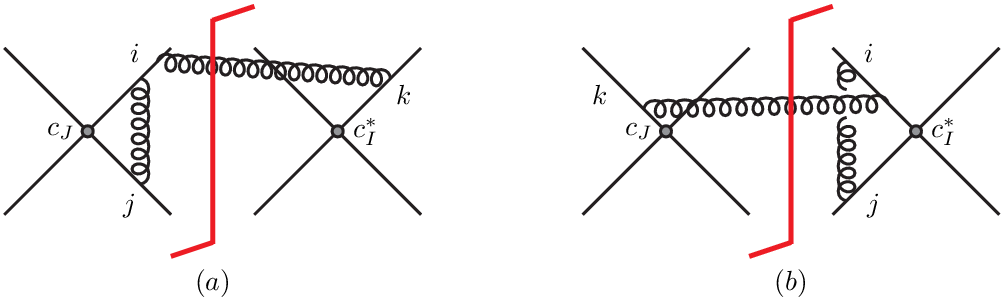
\includegraphics[width=0.7\textwidth]{plots/diagram4-pecjak.png}
  \end{center}
  \caption{
    Three-Wilson-line, mixed real-virtual integrals, which add up to scaleless
    integral.
  }
  \label{fig:pecjak4}
\end{figure}
%

The single-gluon cut integrals of Fig.~\ref{fig:pecjak4} read
%
\begin{eqnarray}
  \bar{I}_{8, ijk}^{(a)} &= &
  n_i \cdot n_j\; n_i \cdot n_k\; 
  \int d^d k\, d^d l\; 
  \frac{\delta_+(k^2) \,
    \; \delta^{(2)}(q_\perp-k_\perp)}
    {(n \cdot k)^\alpha\; (n \cdot l)^\beta \; 
    n_i \cdot k \; n_i \cdot (k+l) \; n_j \cdot l \; n_k \cdot k} \,,
  \\
  \bar{I}_{8, ijk}^{(b)} &= &
  n_i \cdot n_j\; n_i \cdot n_k\; 
  \int d^d k\, d^d l\; 
  \frac{\delta_+(k^2) \,
    \; \delta^{(2)}(q_\perp-k_\perp)}
    {(n \cdot k)^\alpha\; (n \cdot l)^\beta \; 
    n_i \cdot l \; n_i \cdot (k+l) \; n_j \cdot l \; n_k \cdot k} \,.
  %\label{eq:}
\end{eqnarray}
%
This type of diagrams are scaleless and vanish in the fully massless case
discussed in~\cite{Ferroglia:2012uy} but they do not need to vanish here as in
our case two outgoing legs are massive. 


%-----------------------------------------------------------------------------
\newpage
\section{Boundary terms}

We would like to perform sector decomposition of the following integral
of the prototype PR43
%
\begin{equation}
  I = 
  \int \frac{d^d k\, d^d l\, \delta(k^2) \delta(l^2)\,
             \delta(|k_\perp+l_\perp|^2-1)}
  {(n\cdot k)^{\alpha+1} (n\cdot l)^\alpha (v_3 \cdot l) (k\cdot l)}\,,
  %\label{eq:}
\end{equation}
%
taken at the boundary, which corresponds to $\beta=1$ (or, equivalently $x=1$).

The boundary integral can be parameterized with $k_+$, $k_-$, $l_+$, $l_-$,
$k_T$, $l_T$ and $\phi$, where the latter is the angle between transverse
components of gluons four-momenta. The integration measures in the transverse
plane read
%
\begin{eqnarray}
  d^{d-2} k_\perp & = & 
  \Omega_{1-2\epsilon}\,
  k_T^{1-2\epsilon} \sin^{-2\epsilon}\! \phi\, d k_T\, d\phi\,,
  \\
  d^{d-2} l_\perp & = & 
  \Omega_{2-2\epsilon}\,
  l_T^{1-2\epsilon} d l_T\,.
  %\label{eq:}
\end{eqnarray}
%
\smallcomment{Possible issue with factor 1/2 related to $[0,2\pi]$ range of
$\phi$.}\\
%
It is convenient to replace the angular variable $\phi$ by
%
\begin{equation}
  \eta = \frac{1-\cos\phi}{2}\,.
  %\label{eq:}
\end{equation}
%
Then, the whole measure takes the form
%
\begin{equation}
  d^d k\, d^d l =
  4^{-\epsilon}
  \Omega_{1-2\epsilon}\,
  \Omega_{2-2\epsilon}\;
  k_T^{1-2\epsilon} \,
  l_T^{1-2\epsilon} 
  \big((1-\eta)\eta \big)^{-\frac12-\epsilon}
  dk_+ dk_- dl_+ dl_-
  d k_T\, 
  d l_T\,
  d\eta\,.
  %\label{eq:}
\end{equation}
%
After performing integrations over $k_-$, $l_-$ and $\eta$, we are left with
the following form of the boundary integral
%
\begin{equation}
  I =
  \Sigma
  \int dk_+ dl_+ dk_T dl_T
  \frac{k_+^{-1-\alpha}\, l_+^{1-\alpha} k_T l_T \,
  \Big\{\big[1-(k_T-l_T)^2\big]\big[1-(k_T+l_T)^2\big]
  \Big\}^{-\frac12-\epsilon}
  }{(l_+^2+l_T^2)
  \big(k_T^2 k_+ l_+ +l_T^2 k_+ l_+ + k_T^2 l_+^2 + l_T^2 k_+^2 - k_+ l_+
  \big)
  }\,,
  %\label{eq:}
\end{equation}
%
where $\Sigma$ contains all the constants and the $\delta$ functions generated
the following relations
%
\begin{equation}
  k_- = \frac{k_T^2}{k_+}\,, \qquad \qquad
  l_- = \frac{l_T^2}{l_+},
  %\label{eq:}
\end{equation}
%
and
\begin{equation}
  | k_T - l_T | \leq 1\,,
  \qquad \land \qquad
   k_T + l_T  \geq 1\,.
  \label{eq:kTlT-region}
\end{equation}
%
The last pair of relations defines the integration region in the $(k_T, l_T)$
plane.  This region is depicted in Fig.~\ref{fig:trans-regions}~(left).  The
first inequality in (\ref{eq:kTlT-region}) corresponds to the two solid (red)
lines, while the second inequality corresponds to the dotted (blue) line.

\begin{figure}[t]
  \begin{center}
    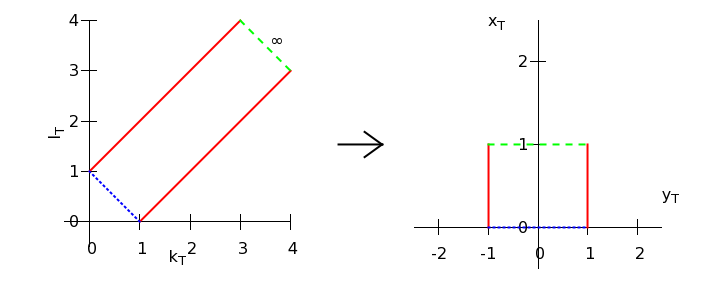
\includegraphics[width=0.99\textwidth]{plots/transverse-phase-space.png}
  \end{center}
  \caption{
  Change of integration region after transformation of transverse coordinates.
  }
  \label{fig:trans-regions}
\end{figure}

The integral $I$ is divergent in the following cases:
%
\begin{enumerate}
  \item
    $k_+ \to 0$, 
    rapidity divergence for gluon $g(k)$
  \item 
    $k_+ \to 0,\ l_+ \to 0$, ???
  \item
    $l_+ \to 0,\ l_T \to 0$, 
    soft divergence for gluon $g(l)$
  \item
    $k_T \to \displaystyle \frac{k_+ }{k_+ + l_+},
    \ l_T \to \frac{l_+ }{k_+ + l_+}$,
    collinear divergence of 3-gluon vertex
\end{enumerate}
%
Let us call the cases 3. and 4. the ``mixed divergences''.

We would like to transform the integration region in the $(\kp, \lp, k_T, l_T)$
space into a hyper-cube and, if necessary, split it such that each of resulting
integrals $\int \prod_i d x_i f(\{x_i\})$ has singularities only in the limits
$x_i \to 0$.
%
We achieve the above in the following steps:
 
%------------------------------------
\subsubsection*{Step 1}

The transverse variables $(k_T, l_T)$ are transformed to new variables 
$(x_T, y_T)$ with the following replacements
%
\begin{equation}
  k_T = \frac{1+y_T-x_T y_T}{2(1-x_T)}\,,
  \qquad \qquad
  l_T = \frac{1-y_T+x_T y_T}{2(1-x_T)}\,,
  %\label{eq:}
\end{equation}
%
and the inverse transformation reads
\begin{equation}
  x_T = 1-\frac{1}{k_T+l_T}\,,
  \qquad \qquad
  y_T = k_T-l_T\,.
  %\label{eq:}
\end{equation}

This results in change of the integration region from the one shown in
Fig.~\ref{fig:trans-regions}~(left) to that of
Fig.~\ref{fig:trans-regions}~(right). The latter corresponds to
%
\begin{equation}
  0 \leq x_T \leq 1
  \qquad \land \qquad
  -1 \leq y_T \leq 1\,.
  %\label{eq:}
\end{equation}

The mixed divergences  now happen at
%
\begin{enumerate}
  \setcounter{enumi}{2}
  \item
    $l_+ \to 0,\ x_T \to 0,\ y_T \to 1$,
  \item
    $x_T \to 0,\ y_T \to \displaystyle \frac{\kp-\lp}{\kp+\lp}$\,.
\end{enumerate}
%
The last divergence occurs on a manifold inside the integration region. This
manifold is depicted in Fig.~\ref{fig:yTmanifold}.

\begin{figure}[t]
  \begin{center}
    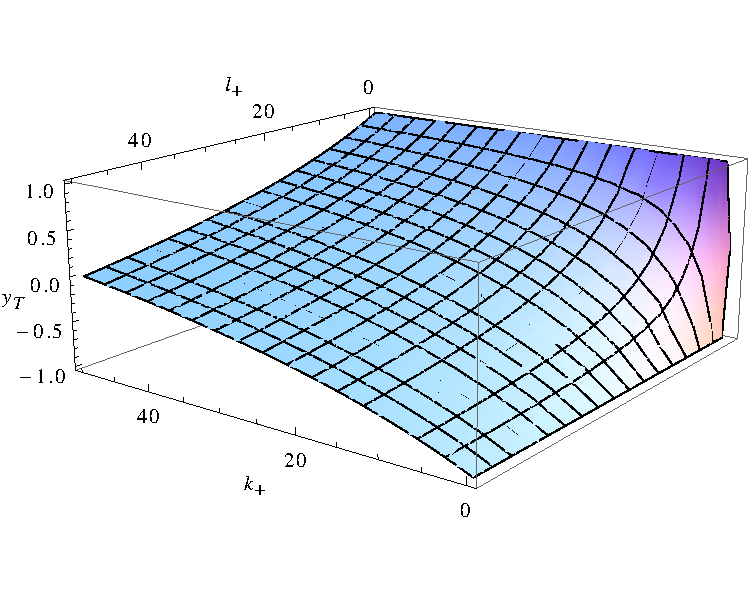
\includegraphics[width=0.49\textwidth]{plots/yTmanifold.pdf}
  \end{center}
  \caption{
  Manifold where the boundary integral becomes singular.
  }
  \label{fig:yTmanifold}
\end{figure}

%------------------------------------
\subsubsection*{Step 2}

In order to transform the manifold singularity into endpoint singularity, we
split the integration region in variable $y_T$ precisely on the manifold of
Fig.~\ref{fig:yTmanifold}
%
\begin{eqnarray}
  I & =  & 
  \int_0^\infty\!\!\! d\kp
  \int_0^\infty\!\!\! d\lp
  \int_0^1\!\!\! d x_T
  \int_{-1}^1\!\!\! d y_T\
  \tilde I(\kp, \lp, x_T, y_T)
  \nonumber \\
  & = &
  \int  d\kp d\lp d x_T
  \int_{-1}^{c(\kp, \lp)}\!\!\! d y_T\
  \tilde I(\kp, \lp, x_T, y_T)
  +
  \int  d\kp d\lp d x_T
  \int_{c(\kp, \lp)}^{1}\!\!\! d y_T\
  \tilde I(\kp, \lp, x_T, y_T)
  \nonumber \\
  & \equiv &
  I_d + I_u\,,
  %\label{eq:}
\end{eqnarray}
%
where
%
\begin{equation}
  c(\kp, \lp) = \frac{\kp-\lp}{\kp+\lp}\,.
  %\label{eq:}
\end{equation}

Now, we use two different parametrizations
%
\begin{equation}
  y_T = \frac{\kp-\lp + 2 \lp \bar y_T}{\kp+\lp}\,,
  \qquad \qquad
  \bar y_T = \frac{y_T-c(\kp,\lp)}{1-c(\kp,\lp)},
  \qquad 
  \text{for}\quad I_u\,,
  %\label{eq:}
\end{equation}
%
and
%
\begin{equation}
  y_T = \frac{\kp-\lp - 2 \lp \bar y_T}{\kp+\lp}\,,
  \qquad
  \bar y_T = \frac{y_T-c(\kp,\lp)}{-1-c(\kp,\lp)},
  \qquad \qquad
  \text{for}\quad I_d\,.
  %\label{eq:}
\end{equation}
%
Hence, we obtain
%
\begin{eqnarray}
 I_d  & =  &
  \int_0^\infty\!\!\! d\kp
  \int_0^\infty\!\!\! d\lp
  \int_0^1\!\!\! d x_T
  \int_{0}^1\!\!\! d \bar y_T\
  \tilde I_1(\kp, \lp, x_T, \bar y_T)\,,
  \\
 I_u  & =  &
  \int_0^\infty\!\!\! d\kp
  \int_0^\infty\!\!\! d\lp
  \int_0^1\!\!\! d x_T
  \int_{0}^1\!\!\! d \bar y_T\
  \tilde I_2(\kp, \lp, x_T, \bar y_T)\,.
  %\label{eq:}
\end{eqnarray}

With the above changes, the mixed singularities happen at
%
\begin{enumerate}
  \setcounter{enumi}{2}
  \item
    $l_+ \to 0,\ x_T \to 0,\ \bar y_T \to 1$,
  \item
    $x_T \to 0,\ \bar y_T \to 0$
\end{enumerate}
%
for $I_u$ and
%
\begin{enumerate}
  \setcounter{enumi}{2}
  \item
    $x_T \to 0,\ \bar y_T \to 0$
\end{enumerate}
%
for $I_d$ and.
%
We see that, in the case of $I_u$, the integral can be divergent at both ends of
$\bar y_T$.

%------------------------------------
\subsubsection*{Step 3}

In order to move all singularities to the limit $x_i \to 0$, we split $I_u$ at 
$\bar y_T = \frac12$
%
\begin{equation}
 I_u = \int_0^1 d \bar y_T\, \tilde I =
 \int_0^\frac12 d \bar y_T\, \tilde I +
 \int_\frac12^1 d \bar y_T\, \tilde I \equiv I_{u0} + I_{u1}\,.
  %\label{eq:}
\end{equation}
%
Then, we apply the following transformations
%
\begin{equation}
  \tilde y_T = 2(1-\bar y_T)\,,
  \qquad \qquad
  \bar y_T = 1-\frac{\tilde y_T}{2}\,,
  \qquad 
  \text{for}\quad I_{u1}\,,
  %\label{eq:}
\end{equation}
%
and
%
\begin{equation}
  \tilde y_T = 2 \bar y_T\,,
  \qquad \qquad
  \bar y_T = \frac{\tilde y_T}{2}\,,
  \qquad 
  \text{for}\quad I_{u0}\,.
  %\label{eq:}
\end{equation}
%
At this point, we have the following mixed singularities:

\begin{displaymath}
  \begin{array}{ll}
   \text{for }  I_{u1}: &
   l_+ \to 0,\ x_T \to 0,\ y_T \to 0,
   \\
    \text{for } I_{u0} \text{ and } I_d: &
    x_T \to 0,\  y_T \to 0\,,
    \\[0.5em]
  \end{array}
\end{displaymath}
 
\noindent
where we dropped tildes and bars for simplicity of notation.

%------------------------------------
\subsubsection*{Step 4}

In the last step, we compress the ranges of the $\kp$ and $\lp$ integrals by the
transformation
%
\begin{equation}
  \kp = \frac{x}{1-x}\,, 
  \qquad \qquad
  \lp = \frac{y}{1-y}\,, 
\end{equation}
%
whose inverse reads
\begin{equation}
  x = \frac{\kp}{1+\kp}\,, 
  \qquad \qquad
  y = \frac{\lp}{1+\lp}\,.
\end{equation}

Hence, finally, our boundary integral is a sum of three contributions
%
\begin{equation}
  I = I_d + I_{u0} + I_{u1}\,,
  %\label{eq:}
\end{equation}
%
which are singular in the following limits: \vspace{10pt}

\noindent
$I_d$:
%
\begin{enumerate}
  \item
  $x \to 0$\,,
  \vspace{-5pt}
  \item
  $x \to 0,\ y \to 0$\,,
  \vspace{-5pt}
  \item
   $ x_T \to 0,\  y_T \to 0$\,,
\end{enumerate}

\noindent
$I_{u0}$:
%
\begin{enumerate}
  \item
  $x \to 0$\,,
  \vspace{-5pt}
  \item
  $x \to 0,\ y \to 0$\,,
  \vspace{-5pt}
  \item
   $ x_T \to 0,\  y_T \to 0$\,,
\end{enumerate}

\noindent
$I_{u1}$:
%
\begin{enumerate}
  \item
  $x \to 0$\,,
  \vspace{-5pt}
  \item
  $x \to 0,\ y \to 0$\,,
  \vspace{-5pt}
  \item
   $y \to 0,\ x_T \to 0,\ y_T \to 0$\,.
\end{enumerate}

%-----------------------------------------------------------------------------
\section{Symmetries between integrals}

Our double-cut, soft function integrals have the general structure
%
\begin{align}
I(\{p_i\}) &= \int d^dk\, d^d l\, \delta^{(+)}(k^2) \delta^{(+)}(l^2)
     h(p_i\cdot p_j, p_i\cdot k, p_i \cdot l)\,
     \delta(1-|k_\perp+l_\perp|)\,.
\end{align}
%
Because of the transverse delta function, these integrals are invariant
only under a subgroup of the Lorentz group which involves:
%
\begin{itemize}
  %\setlength\itemsep{1.2em}
  \item
  rescaling of the light-cone components of the momenta $k$ and $l$ compensated
  by inverse rescaling of the light-cone components of the external momenta,
  \item
  rotations of the above momenta in the transverse plane.
\end{itemize}
%
Let us denote
\begin{align}
  p\cdot q & \quad \text{usual, $d$-dimensional scalar product}\,, \\
  p * q & = p_0 q_0 - p_3 q_3 = p_+ q_- + p_- q_+\,.
\end{align}


\begin{enumerate}
  \item
  Given the above, reduced Lorentz symmetry, and the fact that the result can
  only depend on external momenta, we conclude, that our integral must be a
  function of $p_i * p_j$ and $p_{i,\perp} \cdot p_{j,\perp}$ or, equivalently,
  $p_i * p_j$ and $p_i \cdot p_j$.

  \item
  The integrand is invariant under the rescaling of $p_3 = \lambda_3 p_3$
  and $p_4 = \lambda_4 p_4$, which means that the result can only be a function
  of ratios of the above scalar products.

  \item
  Integrals which do not exhibit $\alpha$ poles are also invariant under
  rescaling of $p_1$. But, here, one cannot form a variable of the type $p_1
  \cdot p_3/\sqrt{p_1^2 p_3^2}$ because $p_1$ is massless. As a consequence, the
  only possibility is $p_3^{*2}/p_3^2 = p_4^{*2}/p_4^2 $. This is why some
  abelian integrals $13$ and $14$ are equal.

  \item
  In case with $\alpha$ poles, rescaling of $p_1$ is broken 
  %
  \begin{displaymath}
    I(\lambda p_1) =  \lambda^{-\alpha} I(p_1)\,,
  \end{displaymath}
  %
  but its form can be
  deduced from  the integrand. For example, for the case of graphs involving
  lines 1 and 3, the above means that the only way $p_1$ can enter is through a
  prefactor and 
  %
  \begin{displaymath}
    I(\{p_i\}) =  \left(\frac{p_1\cdot p_3}{\sqrt{p_3^2}}\right)^{-\alpha} 
    I(\{p_i\}\backslash \{p_1\})\,.
  \end{displaymath}
  (Possibly also $\left(p_1\cdot p_3/\sqrt{p_3^{*2}}\right)^{-\alpha}$.)

\end{enumerate}


%-----------------------------------------------------------------------------
\chapter{Renormalization}

%-----------------------------------------------------------------------------
\section{Beam functions from RGE}

We define
%
\begin{equation}
  I_{ij}(z,\Lp) = I^{(0)}(z,\Lp) +
  \asp I^{(1)}_{ij}(z,\Lp) + \left(\asp\right)^2 I^{(2)}_{ij}(z,\Lp) + \ldots\,.
  %\label{eq:}
\end{equation}
%
From RGE we obtain
%
\begin{subequations}
  %\label{eq:}
  \begin{align}
  I^{(0)}_{ij}(z,\Lp) & = 
  \delta_{ij} \delta(1-z)\,,\\
  %
  I^{(1)}_{ij}(z,\Lp) & = 
  \left[\Gamma^{(0)}_i \frac{\Lp^2}{4} - \gamma^{(0)}_i \Lp \right]
  \delta_{ij} \delta(1-z) - P^{(0)}_{ij} (z) \Lp + R^{(0)}_{ij}(z)\,, \\
  \\
  %
  I^{(2)}_{ij}(z,\Lp) & = 
  \left[
  \left(\Gamma^{(0)}_i\right)^2 \frac{\Lp^4}{32}
  -\Gamma^{(0)}_i\left(3\gamma^{(0)}_i 
  - \beta_0 \right) \frac{\Lp^3}{12}
  + \gamma^{(0)}_i\left(\gamma^{(0)}_i - \beta_0 \right)\frac{\Lp^2}{2}
  \right] \delta_{ij} \delta(1-z) 
  \nonumber \\
  & 
  -\Gamma^{(0)}_i P^{(0)}_{ij} \frac{\Lp^3}{6} 
  +\Gamma^{(0)}_i R^{(0)}_{ij} \frac{\Lp^2}{4} 
  +\left(\gamma^{(0)}_i -\beta_0\right) P^{(0)}_{ij} \frac{\Lp^2}{2} 
  -\left(\gamma^{(0)}_i -\beta_0\right) R^{(0)}_{ij} \Lp
  \nonumber \\
  & 
  + \left[
  \Gamma^{(1)}_i \frac{\Lp^2}{4}-\gamma^{(1)}_i \Lp
  \right] \delta_{ij} \delta(1-z)
  - P^{(1)}_{ij}(z)\Lp
  -\left[
  \Gamma^{(0)}_i \frac{\Lp^3}{12}-\gamma^{(0)}_i \frac{\Lp^2}{2}
  \right] P^{(0)}_{ij}(z) 
  \nonumber \\
  &
  + D_{ij}(z)\frac{\Lp^2}{2} - E_{ij}(z) \Lp + R^{(1)}_{ij}(z)\,.
  \end{align}
\end{subequations}
%
The anomaly exponent reads
\begin{equation}
  g_i (\Lp,\as) =  
  - \left(\ln \frac{M^2}{\mu^2} + \Lp\right) F_{i\bar i}(\Lp,\as)\,,
  %\label{eq:}
\end{equation}
%
with
%
\begin{equation}
  F_{i\bar i}(\Lp,\as) = 
  \asp \Gamma^{(0)}_i \Lp + 
  \left(\asp\right)^2 
  \left( \Gamma^{(0)}_i \frac{\beta_0}{2}\Lp^2 +\Gamma^{(1)}_i \Lp + d_{i,2}
  \right)\,.
  %\label{eq:}
\end{equation}
%
With the above, we define
%
\begin{equation}
  C_{i\bar i \gets a b} = 
  e^{g_i (\Lp, \as)}\, I_{ia}(z_1,\Lp, \as)\, I_{\bar i b}(z_2,\Lp, \as) \,
  {\rm HS}_{\iibar}(\Lp, \as)
  %\label{eq:}
\end{equation}


%-----------------------------------------------------------------------------
\subsection{Leading logarithmic coefficient in $qg \to gg$ channel}

The highest term this case is $\Lp^3$. The coefficient in front gets
contributions from three sources
%

\begin{displaymath}
  \begin{array}{ccc}
    I^{(1)}_{gq} I^{(1)}_{gg} & \mapsto & 
    -\frac{1}{4} \Gamma^{(0)}_g \delta(1-z_2) P^{(0)}_{gq}(z_1)\,, \\[1em]
    %
    I^{(2)}_{gq} I^{(0)}_{gg} & \mapsto & 
    -\frac{1}{4} \Gamma^{(0)}_g \delta(1-z_2) P^{(0)}_{gq}(z_1)\,, \\[1em]
    %
    g_g I^{(1)}_{gq}I^{(0)}_{gg}  & \mapsto & 
    \Gamma^{(0)}_g \delta(1-z_2) P^{(0)}_{gq}(z_1)\,.
    %
  \end{array}
\end{displaymath}
%
Hence, the overall result reads
\begin{equation}
    C_{gg\gets qg}^\text{LL} = 
    \frac12 \Gamma^{(0)}_g\, \delta(1-z_2)\, P^{(0)}_{gq}(z_1)\, \Lp^3\,,
  %\label{eq:}
\end{equation}
%
which, after Fourier transform corresponding to the
replacement~\cite{Li:2013mia}
%
\begin{equation}
  \Lp^3 \to -\left[\frac{3}{q_T^2} \ln^2\frac{\mu^2}{q_T^2}\right]^{[\mu^2]}_*
  - 4\zeta_3\delta(q_T^2)\,,
  %\label{eq:}
\end{equation}
%
for $q_T>0$, where we keep only the first term in which we can ignore the
'*' prescription, gives
%
\begin{equation}
    C_{gg\gets qg}^\text{LL} = 
    -\frac{3}{2} \Gamma^{(0)}_g\, \delta(1-z_2)\, P^{(0)}_{gq}(z_1)\,
    \frac{1}{q_T^2} \ln^2\frac{\mu^2}{q_T^2}\,.
  %\label{eq:}
\end{equation}
  



%-----------------------------------------------------------------------------
\newpage
\section{Soft function from RGE}

%-----------------------------------------------------------------------------
\subsection{Introductory considerations}

The renormalized soft function of small-$q_T$ factorization satisfies the
following RGE equation~\cite{Zhu:2012ts}
%
\begin{equation}
  \frac{d}{d\ln \mu} \bfS_\iibar (\mu) =
  - \bfgamma^{s \dagger}_\iibar \,\bfS_\iibar (\mu)  
  - \bfS_\iibar (\mu)\, \bfgamma^{s}_\iibar \,,
  \label{eq:SF-RGE-main}
\end{equation}
%
where
%
\begin{equation}
  \bfgamma^{s}_\iibar = \bfgamma^{h}_\iibar - 2 \gamma^{i} \bfI\,,
  %\label{eq:}
\end{equation}
%
and $\bfgamma^{h}_\iibar$ is defined as a non-$\Gamma_\text{cusp}$ part of the
full anomalous dimension matrix $\bfGamma$~\cite{Ahrens:2010zv}, while
$\gamma^{i}$ is the massless-particle anomalous dimension (enters RGE
equations for beam functions in Drell-Yan and Higgs
production~\cite{Becher:2010tm, Becher:2012yn}). To make the notation lighter, to
this end, we shall omit the index $\iibar$, keeping in mind that the soft
function and the anomalous dimension are different in the \qqbar and $gg$
channels.

The soft anomalous dimension matrix $\bfgamma^{s}$ is related to the soft
renormalization factor (also a matrix in colour space), $\bfZ_s$, as follows
%
\begin{equation}
  \bfgamma^{s} = - \bfZ_s^{-1}\frac{d\bfZ_s}{d\ln \mu}\,,
  %\label{eq:}
\end{equation}
%
and $\bfZ_s$ absorbs all UV divergences such that~\footnote{
A quick consistency check:
%
\begin{eqnarray}
  \frac{d}{d\ln \mu} \bfS(\mu) 
  = 
  \frac{d\bfZ^\dagger_s}{d\ln\mu} \bfS_\bare \bfZ_s +
  \bfZ^\dagger_s \bfS_\bare \frac{d\bfZ_s}{d\ln\mu}
  =
  \underbrace{\frac{d\bfZ^\dagger_s}{d\ln\mu}
  (\bfZ^{-1}_s)^{^\dagger}}_{-\bfgamma^{s \dagger}}
  \underbrace{\bfZ^\dagger_s \bfS_\bare \bfZ_s}_{\bfS(\mu)}
  +
  \underbrace{\bfZ^\dagger_s \bfS_\bare \bfZ_s}_{\bfS(\mu)}
  \underbrace{\bfZ_s^{-1} \frac{d\bfZ_s}{d\ln\mu}} _{-\bfgamma^{s }}\,.
  %\label{eq:}
\end{eqnarray}
}

%
\begin{equation}
  \bfS(\mu) = \bfZ^\dagger_s(\mu,\epsilon) \bfS_\bare(\epsilon)
  \bfZ_s(\mu,\epsilon)\,.
  %\label{eq:}
\end{equation}
%
Each quantity in the above equation has perturbative expansion, either in the
renormalized coupling, $a_s =
\frac{\alpha_s}{4\pi}$, or in the bare coupling,
$a_s^0 = \frac{\alpha_s^0}{4\pi}$, and the relation between the two is
%
\begin{equation}
  a_s^0(\epsilon) = 
  \left(\frac{\mu^2 e^{\gamma_E}}{4\pi}\right)^\epsilon Z_\alpha a_s
  \equiv \xi_\as(\epsilon,\mu)\, Z_\alpha\, a_s (\mu)\,,
\end{equation}
%
where the \msbar renormalization constant reads
%
\begin{equation}
  Z_\alpha = 
  1- \frac{\beta_0 \as}{4\pi \epsilon} + \ldots =
  1- \frac{\beta_0}{\epsilon} a_s(\mu) + \ldots\,.
  \label{eq:Zalpha}
\end{equation}
%
Hence, we can write
%
\begin{eqnarray}
  \bfS(\mu) & = &  
  \bfS^{(0)}(\mu) + a_s(\mu)\, \bfS^{(1)}(\mu) + a_s^2(\mu)\, \bfS^{(2)}(\mu) 
  + \order{a_s^3}
  \nonumber \\
  & = & 
  \left(\bfZ^{\dagger (0)}_s(\epsilon, \mu) + 
  a_s(\mu)\,\bfZ^{\dagger (1)}_s(\epsilon, \mu) + 
  a_s^2(\mu)\,\bfZ^{\dagger (2)}_s(\epsilon, \mu)  \right)
  \nonumber \\ & &
  \times \left(\bfS^{(0)}_\bare(\epsilon) + 
  a_s(\mu)\, \xi_\as(\epsilon, \mu)\, Z_\alpha\, \bfS^{(1)}_\bare(\epsilon) 
  + a_s(\mu)^2\, \xi_\as^2(\epsilon, \mu)\, Z_\alpha^2\,
    \bfS^{(2)}_\bare(\epsilon) \right)
  \\ & &
  \times 
  \left(\bfZ^{(0)}_s(\epsilon, \mu) + a_s(\mu)\,\bfZ^{(1)}_s(\epsilon, \mu) + 
  a_s(\mu)^2\,\bfZ^{(2)}_s(\epsilon, \mu)  \right)\,,
  \nonumber
  %
  %\label{eq:}
\end{eqnarray}
%
and, with Eq.~(\ref{eq:Zalpha}) and $\bfZ_s^{(0)} = \bfI$, we get
%
\begin{eqnarray}
  \bfS(\mu) & = &  
  \bfS^{(0)}(\mu) + a_s(\mu)\, \bfS^{(1)}(\mu) + a_s^2(\mu)\, \bfS^{(2)}(\mu) 
  \nonumber \\
  & = & 
  \left(\bfI + 
  a_s(\mu)\,\bfZ^{\dagger (1)}_s(\epsilon, \mu) + 
  a_s^2(\mu)\,\bfZ^{\dagger (2)}_s(\epsilon, \mu)  \right)
  \nonumber \\ & &
  \times \left(\bfS^{(0)}_\bare(\epsilon) + 
  a_s(\mu)\, \xi_\as \bfS^{(1)}_\bare(\epsilon) -
  a_s(\mu)^2\, \xi_\as\,  \frac{\beta_0}{\epsilon}\, \bfS^{(1)}_\bare(\epsilon) 
  + a_s(\mu)^2\, \xi_\as^2\, 
    \bfS^{(2)}_\bare(\epsilon) \right)
  \nonumber \\ & &
  \times 
  \left(\bfI+ a_s(\mu)\,\bfZ^{(1)}_s(\epsilon, \mu) + 
  a_s(\mu)^2\,\bfZ^{(2)}_s(\epsilon, \mu)  \right)\,,
  \nonumber
  %
  %\label{eq:}
\end{eqnarray}
%
which  gives us the following, order-by-order relations
%
\begin{eqnarray}
  \bfS^{(0)} & = &  \bfS^{(0)}_\bare \,,
  \\[0.5em]
  \bfS^{(1)} & = &
  \bfZ^{\dagger (1)}_s \bfS^{(0)}_\bare  + \bfS^{(0)}_\bare \bfZ^{(1)}_s  +
  \xi_\as \bfS^{(1)}_\bare \,,
  \\[0.5em]
  \bfS^{(2)} & = &
  \bfZ^{\dagger (2)}_s \bfS^{(0)}_\bare  + \bfS^{(0)}_\bare \bfZ^{(2)}_s  +
  \bfZ^{\dagger (1)}_s \bfS^{(0)}_\bare \bfZ^{(1)}_s 
  \nonumber \\[0.5em]
  & &
  + \bfZ^{\dagger (1)}_s \xi_\as \bfS^{(1)}_\bare  + 
  \xi_\as \bfS^{(1)}_\bare \bfZ^{(1)}_s  +
  \xi_\as^2 \bfS^{(2)}_\bare 
  -\frac{\beta_0}{\epsilon}\, \xi_\as \bfS^{(1)}_\bare
  \,.
  \label{eq:S2ren}
\end{eqnarray}
%
The quantities on the l.h.s. are $\epsilon$-independent. The $\bfZ^{(i)}_s$
factors have only singular terms with poles in $\epsilon$, while the bare
functions, $\bfS^{(1)}_\bare$ and $\bfS^{(2)}_\bare$, have both singular and
finite parts.

We can now absorb the $\xi_\as$ prefactors into the definitions of the bare
soft functions and change the notation according to
%
\begin{equation}
  \tbfS^{(n)}_\bare \equiv \xi_\as^n \bfS^{(n)}_\bare\,.
  %\label{eq:}
\end{equation}
%

Specifically, at the order $a_s^2$, from Eq.~(\ref{eq:S2ren}), we get
%
\begin{eqnarray}
  \underbrace{\bfS^{(2)}}_{\text{finite part only}}   
  &  =  &
  \overbrace{\bfZ^{\dagger (2)}_s \tbfS^{(0)}_\bare  + 
   \tbfS^{(0)}_\bare \bfZ^{(2)}_s  +
   \bfZ^{\dagger (1)}_s \tbfS^{(0)}_\bare \bfZ^{(1)}_s}^{\text{(I) pole part only}} 
  \nonumber \\
  & &
  \quad +  \quad 
  \underbrace{\bfZ^{\dagger (1)}_s \tbfS^{(1)}_\bare  + 
  \tbfS^{(1)}_\bare \bfZ^{(1)}_s  +
  \tbfS^{(2)}_\bare
 -\frac{\beta_0}{\epsilon}\, \tbfS^{(1)}_\bare
  }_{\text{(II) finite + pole part}} \,.
  \label{eq:renS2}
\end{eqnarray}
%
The  part (I) on the r.h.s. has only terms singular in $\epsilon$, which come
from the fact that the $\bfZ_s$ factors are defined in the \msbar scheme. 

These pole terms have to cancel against singular terms of part (II). And that
can be used in the following way:
%
Knowing $\bfZ_s^{(1)}$ and $\bfZ_s^{(2)}$, as well as $\tbfS^{(0)}_\bare$ and
$\tbfS^{(1)}_\bare$, allows one to cross-check all the singular terms of
the $\tbfS^{(2)}_\bare$ function obtained from direct calculation.

To this end, for notational simplicity, we abandon tilde in the soft function
symbol and assume that the latter always includes the appropriate power of
$\xi_\as$.

%Assuming that all the pole terms cancel, as they should, we have
%%
%\begin{equation}
%  \bfS^{(2)} = 
%  \left[\bfZ^{\dagger (1)}_s \bfS^{(1)}_\bare\right]_{\text{finite part}}  + 
%  \left[\bfS^{(1)}_\bare \bfZ^{(1)}_s\right]_{\text{finite part}}  +
%  \left[\bfS^{(2)}_\bare\right]_{\text{finite part}}\,,
%\end{equation}
%% 
%and we can use the already known results for
%$\bfS^{(1)}_\bare$ and  $\bfZ^{(1)}_s$ to determine the RG-induced part of
%$\bfS^{(2)}$. For that we do not even need to know $\bfZ^{(2)}_s$.


%%
%\begin{eqnarray}
%  \overbrace{\bfS^{(2)}}^{\text{finite part only}}  & =  &
%  \overbrace{\bfZ^{\dagger (2)}_s \bfS^{(0)}_\bare  + \bfS^{(0)}_\bare \bfZ^{(2)}_s  +
%  \bfZ^{\dagger (1)}_s \bfS^{(0)}_\bare \bfZ^{(1)}_s}^{\text{pole part only}} 
%  %\nonumber \\
%  %& &
%  %+ \
%  \underbrace{\bfZ^{\dagger (1)}_s \bfS^{(1)}_\bare  + \bfS^{(1)}_\bare \bfZ^{(1)}_s  +
%  \bfS^{(2)}_\bare}_{\text{finite + pole part}} \,.
%  %\label{eq:}
%\end{eqnarray}

%-----------------------------------------------------------------------------
\subsection{Determination of $\mathbold{L_\perp^n}$-dependent terms of the soft
function}
\label{sec:RGevolution}


The RGE evolution equation (\ref{eq:SF-RGE-main}) can be written as
%
\begin{equation}
  \frac{d}{d L_\perp} \bfS(\mu) =
  - \frac{1}{2} \left[
  \bfgamma^{s \dagger}\,\bfS(\mu)  
  + \bfS(\mu)\, \bfgamma^{s}
  \right]\,,
  \label{eq:SF-RGE-Lp}
\end{equation}
%
where
%
\begin{equation}
  L_\perp = \ln\frac{\mu^2 x_T^2}{b_0^2}
  \qquad \qquad
  \text{and}
  \qquad \qquad
  b_0 =  2 e^{- \gamma_E}\,.
  %\label{eq:}
\end{equation}
%
Both the soft function and the anomalous dimension have perturbative expansions
%
\begin{eqnarray}
  \bfS  & = &
  \bfS^{(0)} + a_s \bfS^{(1)} + a_s^2 \bfS^{(2)} + \ldots\,,
  \label{eq:Sren-exp}
  \\
  \bfgamma_{s} & = &
  a_s \left(\bfgamma_{s,0} + a_s \bfgamma_{s,1}+ \ldots\right)\,.
  \label{eq:gammas-exp}
\end{eqnarray}
%
All quantities in the above equations are renormalized and in 4 dimensions.
 
Because the anomalous dimension matrix starts at the order $a_s$,
Eq.~(\ref{eq:SF-RGE-Lp}) can be solved iteratively. We just need to plug
Eqs.~(\ref{eq:Sren-exp}) and (\ref{eq:gammas-exp}) into 
Eq.~(\ref{eq:SF-RGE-Lp}) and  remember that the renormalized, 4-dimensional
coupling $a_s$ also depends on $\ln\mu$, which implies
%
\begin{equation}
  \frac{d a_s}{dL_\perp} = \frac12 \frac{d a_s}{d\ln\mu} = 
  \frac12 \frac{\partial a_s}{\partial \ln\mu} = 
  \frac12 \frac{\beta(a_s)}{4\pi} = 
  - \beta_0\, a_s^2 + \order{a_s^3}\,.
  %\label{eq:}
\end{equation}

After collecting terms at each order, we
arrive at the following differential equations
%
\begin{eqnarray}
  \frac{d}{dL_\perp} \bfS^{(0)} & = &  0\,,
  \\
  \frac{d}{dL_\perp} \bfS^{(1)} & = & 
  -\frac12\left[
  \bfS^{(0)}\, \bfgamma_{s,0} + \bfgamma_{s,0}^\dagger\, \bfS^{(0)} 
  \right]\,,
  \\
  \frac{d}{dL_\perp} \bfS^{(2)} & = & 
  -\frac12\left[
  \bfS^{(1)}\, \bfgamma_{s,0} + \bfgamma_{s,0}^\dagger\, \bfS^{(1)}  
  - 2 \beta_0 \bfS^{(1)}  +
  \bfS^{(0)}\, \bfgamma_{s,1} + \bfgamma_{s,1}^\dagger\, \bfS^{(0)} 
  \right]\,.
  %\label{eq:}
\end{eqnarray}
 
Hence, knowing the soft anomalous dimension to the order $a_s^2$, and the soft
function to the order~$a_s^1$ allows one to determine all pieces of the soft
function at the order $a_s^2$ except the constant term. Specifically, we get
%
\begin{eqnarray}
  \bfS^{(2)} 
  & = & 
  -\frac12\Bigg\{
  \frac12\left[
  \bfS^{(1)}_{L_\perp}\, \bfgamma_{s,0} + 
  \bfgamma_{s,0}^\dagger\, \bfS^{(1)}_{L_\perp}  
  - 2 \beta_0 \bfS^{(1)}_{L_\perp}  +
  \bfS^{(0)}\, \bfgamma_{s,1} + \bfgamma_{s,1}^\dagger\, \bfS^{(0)} 
  \right] L_\perp^2
   \\
  & &
  \hspace{25pt} + \left[
  \bfS^{(1)}_\text{const}\, \bfgamma_{s,0} + 
  \bfgamma_{s,0}^\dagger\, \bfS^{(1)}_\text{const}  
  - 2 \beta_0 \bfS^{(1)}_\text{const}  +
  \bfS^{(0)}\, \bfgamma_{s,1} + \bfgamma_{s,1}^\dagger\, \bfS^{(0)} 
  \right] L_\perp
  \Bigg\} 
  + \text{const}\,,
  \nonumber
  %\nonumber \\
  %& &
  %+ \text{const}.
  %\label{eq:}
\end{eqnarray}
%
where $\bfS^{(1)}_{L_\perp}$ and $\bfS^{(1)}_\text{const}$ denote, respectively,
the $L_\perp$-dependent and $L_\perp$-independent pieces of the $\bfS^{(1)}$
soft function.

%-----------------------------------------------------------------------------
\section{HS functions}

The soft and the hard functions enter the cross section through the trace of
their product
%
\begin{equation}
  \text{Tr} \left[\mathbold{H}_{\iibar}(M, m_t, \cos\theta, \mu) 
                  \mathbold{S}_{\iibar}(M, m_t, \cos\theta, \LT)\right] = 
  \frac{3\as^2}{8 d_i} \sum_{n=0}  \sum^{n}_{m=0}
  \left(\asp\right)^n \LT^m\,
  \text{HS}^{(n,m)}_\iibar\,.
  %\label{eq:}
\end{equation}
%
The only source of $\LT$ is the soft function. Hence, we have the following
contributions
%
\begin{align}
  \text{HS}^{(0,0)} & 
  \quad \leftarrow  \quad \mathbold{H}^{(0)} \mathbold{S}^{(0,0)}\,, \\
  \text{HS}^{(1,1)} & 
  \quad \leftarrow  \quad \mathbold{H}^{(0)} \mathbold{S}^{(1,1)}\,, \\
  \text{HS}^{(1,0)} & 
  \quad \leftarrow  \quad \mathbold{H}^{(0)} \mathbold{S}^{(1,0)},\ 
	                  \mathbold{H}^{(1)} \mathbold{S}^{(0,0)}\,, \\
  \text{HS}^{(2,2)} & 
  \quad \leftarrow  \quad \mathbold{H}^{(0)} \mathbold{S}^{(2,2)}\,, \\
  \text{HS}^{(2,1)} & 
  \quad \leftarrow  \quad \mathbold{H}^{(0)} \mathbold{S}^{(2,1)},\ 
	                  \mathbold{H}^{(1)} \mathbold{S}^{(1,1)}\,.
\end{align}


%-----------------------------------------------------------------------------
\section{Anomalous dimension}

A velocity-dependent part of the anomalous dimension can be written in a compact
form as~\cite{Ferroglia:2009ii, Kidonakis:2009ev}
%
\begin{eqnarray}
   \label{eq:vel-dep-ad}
   \gamma_{\rm cusp}(\beta,\alpha_s)
   &=& \gamma_{\rm cusp}(\alpha_s)\,\beta\coth\beta \nonumber\\
   &&\hspace{-22mm}\mbox{}+ \frac{C_A}{2} 
    \left( \frac{\alpha_s}{\pi} \right)^2 
    \Bigg\{ \frac{\pi^2}{6} + \zeta_3 + \beta^2 
    + \coth^2\beta \left[ \mbox{Li}_3(e^{-2\beta}) 
    + \beta\,\mbox{Li}_2(e^{-2\beta}) - \zeta_3 
    + \frac{\pi^2}{6}\,\beta + \frac{\beta^3}{3} \right] \\
   &&\quad\mbox{}+ \coth\beta \left[ 
    \mbox{Li}_2(e^{-2\beta}) - 2\beta\,\ln(1-e^{-2\beta}) 
    - \frac{\pi^2}{6}\,(1+\beta) - \beta^2 - \frac{\beta^3}{3} 
    \right] \Bigg\}
    + {\cal O}(\alpha_s^3) \,, \nonumber
\end{eqnarray}
%
where $\beta$ is a cusp angle discussed below.


%------------------------------------
\subsection{Cusp angles}

The amplitudes are functions of \emph{Lorentz invariants}~\cite{Becher:2009kw}
%
\begin{equation}
  s_{ij} \equiv 2 \sigma_{ij} p_i \cdot p_j + \iep\,,
  \label{eq:sij-def}
\end{equation}
%
and
\begin{equation}
  p_i^2 = m_i^2\,,
  %\label{eq:}
\end{equation}
%
where
%
\begin{eqnarray}
  \sigma_{ij} = \left\{
    \begin{array}{cl} 
      + 1 &  \text{if } p_i, p_j \text{ are both incoming or outgoing} \\
      - 1 &  \text{otherwise}
    \end{array}
    \right.\,.
  %\label{eq:}
\end{eqnarray}
%
For massive particles we define \emph{four-velocities}
%
\begin{equation}
  v_i \equiv  \frac{p_i}{m_i}\,,
  \qquad \qquad v_i^2 = 1\,.
  %\label{eq:}
\end{equation}
%
We also define \emph{abbreviations}
%
\begin{equation}
  w_{ij} \equiv - \sigma_{ij} v_i \cdot v_j - \iep\,.
  %\label{eq:}
\end{equation}
%
We label massless particles with lowercase $i, j, \ldots$ and massive
ones with capital indices $I, J, \ldots$.

The soft anomalous dimension is a function of \emph{cusp angles}, $\beta_{ij}$, 
$\beta_{Ij}$ and $\beta_{IJ}$, formed by massless and/or massive Wilson lines. They
read~\cite{Becher:2009kw}
%
\begin{subequations}
  %\label{eq:}
  \begin{align}
    \beta_{ij} & = 
    \ln \frac{-2 \sigma_{ij}\, p_i \cdot p_j\, \mu^2}{(-p_i^2)(-p_j^2)} =
    L_i + L_j - \ln\frac{\mu^2}{-s_{ij}}\,,
    \\
    \beta_{Ij} & = 
    \ln \frac{-2 \sigma_{ij}\, v_I \cdot p_j\, \mu}{(-p_j^2)} =
    L_j - \ln\frac{m_I \mu}{-s_{ij}}\,,
    \\
   \label{eq:betaIJ-def}
    \beta_{IJ} & =  {\rm arccosh} \left(w_{IJ}\right) = 
                    {\rm arccosh} \left(\frac{-s_{IJ}}{2 m_I m_J}\right)\,,
  \end{align}
\end{subequations}
%
where we have introduced
%
\begin{equation}
  L_i = \ln \frac{\mu^2}{(-p_i^2)}\,,
  %\label{eq:}
\end{equation}
%
which comes from regularization of IR divergences in effective theory by taking
massless partons slightly off-shell $(-p_i^2) > 0$~\cite{Becher:2009qa}. The
logarithms $L_i$ need to cancel in the final result for the anomalous dimension
matrix.


%------------------------------------
\subsubsection{$\mathbold{\betaIJ}$ in space-like kinematics}

For space-like kinematics of heavy particles (\eg a top quark incoming
and a top quark outgoing), the cusp angle $\beta_{IJ}$ is real. It
can still, however, be chosen to be positive or negative, as the function $\text{arccosh}$
has two branches, even for real argument. 
%
If we look at the first term in Eq.~(\ref{eq:vel-dep-ad}), we notice that it will
be positive regardless of the sign of $\beta_{IJ}$ because $\coth(\beta_{IJ}) >
0$ for $\betaIJ > 0$ and $\coth(\beta_{IJ}) < 0$ for $\betaIJ < 0$.
 
The choice of positive $\betaIJ$ has, however, at least two advantages: (i)
functions that appear in the $\order{\as^2}$ contribution in
Eq.~(\ref{eq:vel-dep-ad}) are real (in the space-like case) and do not require
analytic continuation, as $0 < x < 1$ for $\Li_{2,3}(x)$ and for $\ln(x)$, (ii),
$\coth(\betaIJ)$ has a physical interpretation as an inverse of a relative
velocity between particles $I$ and $J$, $\vIJ$, which reads
%
\begin{equation}
  \coth(\betaIJ) = \frac{1}{\vIJ}\,,
  \label{eq:cothbetaIJ}
\end{equation}
%
where
%
\begin{equation}
  v_{IJ} = \sqrt{1- \frac{4 m_t^4}{s_{IJ}^2}}\,.
  %\label{eq:}
\end{equation}
%
One can show that taking $\betaIJ < 0$ in Eq.~(\ref{eq:vel-dep-ad}), applying
polylogarithm identities and analytic continuation of the logarithm, leaves the
function in Eq.~(\ref{eq:vel-dep-ad}) unchanged~\cite{AnalyticContinuation}.

The choice $\betaIJ>0$ implies $\vIJ > 0$ and this leads to the following
relation between the latter and the $\beta$ function introduced in
Eq.~(\ref{eq:beta-def})~\cite{MyNotes}
%
\begin{equation}
  \vIJ = \frac{2 \beta}{1+\beta^2}\,.
  \label{eq:vIJ-beta-rel}
\end{equation}
%
We notice that~\cite{MyNotes}
%
\begin{equation}
  \beta = \sqrt{\frac{s-1}{s+1}}\,, \qquad \text{where} \qquad 
  s = \frac{\sIJ}{2 m_t^2}\,,
  %\label{eq:}
\end{equation}
%
which means that
%
\begin{equation}
  \begin{array}{lll}
    \text{space-like:}\quad & s < -1 \quad & \beta \in [1,\infty]\,, \\[0.5em]
    \text{time-like:}\quad & s > 1 \quad & \beta \in [0,1]\,.
  \end{array}
  %\label{eq:}
\end{equation}
%
We also note that $\vIJ \in [0,1]$ both in the space-like and in the time-like
case.


Eq.~(\ref{eq:cothbetaIJ}) has a unique solution for the space-like case with
$\betaIJ >0$~\cite{MyNotes}
%
\begin{equation}
  \betaIJ =  -\frac12 \ln \frac{1-\vIJ}{1+\vIJ}\,,
  \label{eq:betaIJ-vIJ}
\end{equation}
%
which, with help of Eq.~(\ref{eq:vIJ-beta-rel}) can be expressed as
%
\begin{equation}
 \betaIJ = -\frac12 \ln\left[\left(\frac{\beta-1}{\beta+1}\right)^2\right]
         = \ln\left[\frac{\beta+1}{\beta-1}\right]\,,
  \qquad \beta \in [1,\infty].
  \label{eq:betaIJ-beta}
\end{equation}

%------------------------------------
\subsubsection{$\mathbold{\betaIJ}$ in time-like kinematics}

We would like to analytically continue $\betaIJ$ to the time-like region which
corresponds to $\sIJ > 0$. The function in Eq.~(\ref{eq:betaIJ-beta}) has a cut
at imaginary axis and, depending whether we cross it in the upper or the
lower half-plane, we get a different result.

The convention is already established in Eqs.~(\ref{eq:sij-def}).
It implies that the invariant $\sIJ$  has a small
positive part which corresponds to analytic continuation over the upper
half-plane. And this means that $\betaIJ$ acquires imaginary part $- i \pi$ in
the time-like region~\cite{AnalyticContinuation}. The real part is identical to
the one of space-like kinematics and at the end we get
%
\begin{equation}
  \betaIJ = \ln\left(\frac{1+\beta}{1-\beta}\right) - i \pi\,,
  \qquad \beta \in [0,1]\,.
  %\label{eq:}
\end{equation}


%%------------------------------------
%\subsection*{Cusp angle of a $\mathbold{t\bar t}$ pair}
%
%Let us now calculate the cusp angle between \ttbar quarks, $\beta_{34}$. We have
%%
%\begin{eqnarray}
%  s_{34} = 2 p_3 \cdot p_4 + \iep
%  %\label{eq:}
%\end{eqnarray}
%%
%and
%%
%\begin{equation}
%  M^2 = (p_3 + p_4)^2 = 2 m_t^2 + 2 p_3 \cdot p_4\,,
%  %\label{eq:}
%\end{equation}
%%
%which gives
%%
%\begin{equation}
%  \beta_{34} = \arccosh\left(\frac{-(M^2 - 2 m_t^2 + \iep)}{2 m_t^2}\right)
%             = \arccosh\left(-\frac{M^2}{2 m_t^2} + 1 - \iep \right)\,.
%  \label{eq:beta34first}
%\end{equation}
%%
%And this can be expressed by $x_s$ defined in Eq.~(\ref{eq:xs-def})~\footnote{
%%
%We have
%%
%\begin{equation}
%  \frac{M^2}{2 m_t^2} = \frac{2}{1-\beta^2}\,,
%  %\label{eq:}
%\end{equation}
%%
%hence, r.h.s of Eq.~(\ref{eq:beta34first}) reads
%%
%\begin{equation}
%  %\label{eq:}
%  -\frac{2}{1-\beta^2} + 1 - \iep = -\frac{1+\beta^2}{1-\beta^2} - \iep\,.
%\end{equation}
%%
%We use the relation $\arccosh\, x = \ln\left(x + \sqrt{x^2-1}\,\right)$ to get
%%
%\begin{equation}
%  \arccosh\left(-\frac{2}{1-\beta^2} + 1 -\iep\right) = 
%  \ln \left(-\frac{2}{1-\beta^2} + 1 -\iep + \sqrt{\frac{4
%  \beta^2}{(1-\beta^2)^2} + \iep}\right) = \ln \left(-\frac{1-\beta}{1+\beta} +
%  \frac{1-\beta^4}{2\beta(1-\beta^2)} \iep \right)\,.
%  %\label{eq:}
%\end{equation}
%%
%In the last step, we expanded the argument of the logarithm in $\epsilon$.  We
%also used the fact that the real part of the argument under $\sqrt{\quad }\,$ is
%positive, hence the function is single-valued.
%}
%%
%\begin{equation}
%  \beta_{34} = \ln\left(-\frac{1-\beta}{1+\beta}+\iep\right) = 
%               \ln\left(-x_s+\iep\right)\,.
%  \label{eq:beta34-res}
%\end{equation}
%%
%Finally the logarithm can be analytically continued to give the result
%%
%\begin{equation}
%  \beta_{34} = \ln x_s  + i \pi - \iep\,.
%  \label{eq:beta34-res}
%\end{equation}
%And this agrees with the note attached to Ref.~\cite{Li:2013mia}.



%-----------------------------------------------------------------------------
\newpage

\appendix

%\chapter{Appendix}
%-----------------------------------------------------------------------------
\chapter{Soft function colour matrices}
\label{app:wmatrices}

The $q\qbar$ channel
%
\begin{eqnarray}
 %%%
 \bfw_{12}^{q\qbar} = \bfw_{34}^{q\qbar} & = &
 - \frac{C_F}{4N}
 \left( \begin{array}{cc}
   4N^2 & 0 \\
   0 & -1 
 \end{array} \right)\,,
 \\[0.5em]
 %%%
 \bfw_{33}^{q\qbar} = \bfw_{44}^{q\qbar} & = &
 \frac{C_F}{2}
 \left( \begin{array}{cc}
   2N & 0 \\
   0 & C_F
 \end{array} \right)\,,
 \\[0.5em]
 %%%
 \bfw_{13}^{q\qbar} = \bfw_{24}^{q\qbar} & = &
 - \frac{C_F}{2}
 \left( \begin{array}{cc}
   0 & 1 \\
   1 & 2 C_F -\frac{N}{2}
 \end{array} \right)\,,
 \\[0.5em]
 %%%
 \bfw_{14}^{q\qbar} = \bfw_{23}^{q\qbar} & = &
 - \frac{C_F}{2N}
 \left( \begin{array}{cc}
   0 & -N \\
   -N & 1 
 \end{array} \right)\,.
\end{eqnarray}


The $gg$ channel
%
\begin{eqnarray}
 %%%
 \bfw_{12}^{gg} & = &
 - \frac{1}{4}
 \left( \begin{array}{ccc}
   4N^2 & 0   & 0 \\
   0    & N^2 & 0 \\
   0    & 0   & N^2-1
 \end{array} \right)\,,
 \\[0.5em]
 %%%
 \bfw_{34}^{gg} & = &
 - 
 \left( \begin{array}{ccc}
   C_F N & 0            & 0 \\
   0     & -\frac{1}{4} & 0 \\
   0     & 0            & -\frac{N^2-4}{4N^2}
 \end{array} \right)\,,
 \\[0.5em]
 %%%
 \bfw_{33}^{gg}  = \bfw_{44}^{gg} & = &
 \frac{C_F}{2N}
 \left( \begin{array}{ccc}
   2N^2  & 0   & 0 \\
   0     & N^2 & 0 \\
   0     & 0   & N^2-4
 \end{array} \right)\,,
 \\[0.5em]
 %%%
 \bfw_{13}^{gg}  = \bfw_{24}^{gg} & = &
 -\frac{1}{8}
 \left( \begin{array}{ccc}
   0  & 4N     & 0 \\
   4N & N^2    & N^2-4 \\
   0  & N^2-4  & N^2-4
 \end{array} \right)\,,
 \\[0.5em]
 %%%
 \bfw_{23}^{gg}  = \bfw_{14}^{gg} & = &
 -\frac{1}{8}
 \left( \begin{array}{ccc}
   0   & -4N     & 0 \\
   -4N & N^2     & -N^2+4 \\
   0   & -N^2+4  & N^2-4
 \end{array} \right)\,.
\end{eqnarray}

%----------------------------
\chapter[$\mathbold{\phi}$ averaging]{$\mathbold{\phi}$ averaging}

We shall see that NLO and NNLO soft functions involve, respectively, the
transverse delta functions $\delta^{(2)}(k_\perp-q_\perp)$ and
$\delta^{(2)}(k_\perp-l_\perp-q_\perp)$.
%
They are relevant if we want to perform averaging over $q_\perp$ azimuthal angle
$\phi$. Let's have a closer look at these functions.

%------------------------------------
\section[NLO: $\delta^{(2)}(k_\perp-q_\perp)$]{NLO: $\mathbold{\delta^{(2)}(k_\perp-q_\perp)}$}

\begin{eqnarray}
  \delta^{(2)}(k_\perp-q_\perp) 
  & = & \delta(k_x-q_x)\delta(k_y-q_y)  \\
  & = & \delta(k_T \cos\theta_2-q_T \cos\phi)
         \delta(k_T \sin\theta_2-q_T \sin\phi) \\
  & = & \delta(k_T \cos\theta_2-q_T \cos\phi)
        \frac{1}{q_T\cos\phi_0} \delta(\phi-\phi_0)\,,
\end{eqnarray}
%
where
%
\begin{equation}
  \phi_0 = \arcsin\left(\frac{k_T\sin\theta_2}{q_T}\right)\,.
\end{equation}
%
We note that
%
\begin{equation}
  \cos \phi_0  = \sqrt{1-\frac{k_T^2\sin^2\theta_2}{q_T^2}}\,,
\end{equation}
%
hence, we can write
%
\begin{eqnarray}
  \delta(k_T \cos\theta_2-q_T \cos\phi_0)
  \frac{1}{q_T\cos\phi_0} \delta(\phi-\phi_0) 
  & = &
  \frac{\delta\left(k_T \cos\theta_2-q_T
  \sqrt{1-\frac{k_T^2\sin^2\theta_2}{q_T^2}}\right)}
  {q_T\sqrt{1-\frac{k_T^2\sin^2\theta_2}{q_T^2}}} \delta(\phi-\phi_0)\,.
  \nonumber \\
\end{eqnarray}
%
To deal with the first delta function we notice that it vanishes for $k_{T} =
q_T$. Calculating the derivative and set the entire denominator at $k_{T} =
q_T$ leads to the result
%
\begin{equation}
  \delta^{(2)}(k_\perp-q_\perp)  =
  \frac{1}{q_T}\delta(k_T-q_T)\delta(\phi-\phi_0)\,.
\end{equation}
%
What is amazing in the result above is that the prefactor on the right hand sued
does not depend on the azimuthal angle of $k_\perp$, that is $\theta_2$. Hence,
integrations over $k_T$ and $\phi$ factorize.
%
The above result can still be rewritten in a slightly more useful form
%
\begin{equation}
  \delta^{(2)}(k_\perp-q_\perp)  =
  2\, \delta(k_T^2-q_T^2)\delta(\phi-\phi_0)\,.
\end{equation}

%------------------------------------
\section[NNLO: $\delta^{(2)}(k_\perp+l_\perp - q_\perp)$]{NNLO: $\mathbold{\delta^{(2)}(k_\perp-l_\perp - q_\perp)}$}


\begin{eqnarray}
  \delta^{(2)}(k_\perp+l_\perp-q_\perp) 
  & = & \delta(k_x+l_x-q_x)\delta(k_y+l_y-q_y)  \nonumber \\
  & = & \delta(k_T \cos\theta_2+l_T \cos\chi_2-q_T \cos\phi)
         \delta(k_T \sin\theta_2+l_T \sin\chi_2-q_T \sin\phi) \nonumber \\
  & = & \delta(k_T \cos\theta_2+l_T\cos\phi_2-q_T \cos\phi)
        \frac{1}{q_T\cos\phi_0} \delta(\phi-\phi_0)\,,
  \label{eq:nnlo-delta2}	 
\end{eqnarray}
%
where
%
\begin{equation}
  \phi_0 = \arcsin\left(\frac{k_T\sin\theta_2+l_T\sin\chi_2}{q_T}\right)\,,
\end{equation}
%
and Eq.~(\ref{eq:nnlo-delta2}) can be written as
%
\begin{equation}
  \delta(k_T \cos\theta_2+l_T\cos\phi_2-q_T \cos\phi_0)
  \frac{1}{q_T\cos\phi_0} \delta(\phi-\phi_0)\,.
\end{equation}
%
To deal with the first delta we look for the roots in $k_T$ and find two of them

\begin{eqnarray}
k_{T0} & = & 
  -\sqrt{\frac{1}{2} l_T^2 \cos \left(2
  \left(\theta _2-\chi
  _2\right)\right)-\frac{l_T^2}{2}+q_T^2}-l_T
   \cos \left(\theta _2-\chi _2\right)\,,
\\
%
k_{T0} & = & 
   \sqrt{\frac{1}{2} l_T^2 \cos \left(2 \left(\theta _2-\chi
   _2\right)\right)-\frac{l_T^2}{2}+q_T^2}-l_T \cos
   \left(\theta _2-\chi _2\right)\,.
\end{eqnarray}
%
Taking the positive solution, substituting it to the derivative of function
under delta and and substituting the value for $\phi_0$ gives
%
\begin{equation}
  \delta^{(2)}(k_\perp+l_\perp-q_\perp)  =
  \frac{\sqrt{2}}{f}\delta(k_T-k_{T0})\delta(\phi-\phi_0)\,.
\end{equation}
where 
%
\begin{eqnarray}
f & =  &
-\cos \left(\theta _2\right) 
\sqrt{l_T
\sin \left(\theta _2-\chi _2\right) \left(\sin \left(2 \theta _2\right) 
\sqrt{\bar f}-2 l_T \cos ^2\left(\theta
      _2\right) \sin \left(\theta _2-
      \chi _2\right)\right)+
      -\bar f \sin ^2\left(\theta_2\right)  +
      2 q_T^2}
\nonumber \\
& &
+ \sin ^2\left(\theta _2\right) \sqrt{\bar f}
+ \frac{1}{\sqrt{2}}\, l_T\sin \left(2 \theta _2\right)
\sin \left(\theta_2-\chi _2\right)\,,
\end{eqnarray}
%
with
%
\begin{eqnarray}
\bar f & = &
-l_T^2 + 2q_T^2 + l_T^2\cos\left[2(\theta_2-\chi_2)\right]\,.
\end{eqnarray}

%-----------------------------------------------------------------------------
\chapter{Difference between us and Antonia at NLO}

At order $\epsilon^1$ in position space, NLO results start to be different
between these two calculations. The difference comes from three sources and it
has to do with working in 2 vs $d-2$-dimensional, transverse space. This
affects:
%
\begin{itemize}
  %\setlength\itemsep{1.2em}
  \item
  averaging over $\phi$,
  \item
  definition of Fourier transform,
  \item
  appearance of transverse delta function.
\end{itemize}

The key formulae can be found in Sec.~\ref{sec:trans-coor-mom} of this notes and
around formula (8.5), page 93 of Antonia's thesis. All, in all, in momentum
space we have
%
\begin{align}
  \tilde I_\text{us} &= 
  \frac{1}{(2\pi)^{\frac{d-2}{2}}} \frac{1}{S_{d-3}}
  \int \ldots (2\pi)^{d-2} \delta^{(d-2)}(\ldots)\,,\\
  %
  \tilde I_\text{An} &= 
  \frac{1}{2\pi} \frac{1}{S_{1}}
  \int \ldots (2\pi)^{2} \delta^{(2)}(\ldots)\,,
\end{align}
%
where $S_1 = 2\pi$.

Hence, in order to correct Antonia's result we need to multiply it by
%
\begin{equation}
  \frac{(2\pi)^{d-2}}{(2\pi)^{\frac{d-2}{2}} S_{d-3}} \,
  \frac{(2\pi)^2}{(2\pi)^2}\,.
  %\label{eq:}
\end{equation}

%-----------------------------------------------------------------------------
\chapter{FAQ}

\section*{Why does the ``IBP integral'' vanish?}

Don't know exactly. Supposed to be explained in the paper
by~\cite{Chetyrkin:1981qh} but it has to do with vanishing of the surface term
in $d$ dimensions.

\section*{Are we worried by integrating the soft function outside its
validity region?}

Contributions from some graphs gives $1/\alpha$, from others $-1/\alpha$ hence,
these regions to not contribute to the soft function. Only that it is convenient
to integrate over them (because then $k^\mu \in (-\infty,\infty)$.


\section*{Why \boldmath{$\alpha$} poles vanish separately for the soft function and for the production of beam functions?}

This has to be the case because, if we think of a production of the Higgs boson,
each beam function exhibits $\alpha$ poles but the have to cancel between the
collinear and the anti-collinear regions. This has to happen as there is nothing
else they could cancel against. No, if the convolution of beam functions, which
are the same for Higgs, top pair and everything else, is free
from $\alpha$ poles, then the soft function has to show the same property. All
the above applies to small-$q_T$ factorization. BTW The fact that $\alpha$ poles
cancel between beam functions is imposed by the fact that for DY, $S = 1$ and
the latter follows from scalelessness of integrals.

%\section*{Why do we get seperate RG equation for each function?}
%
%This follows from the fact that, when the factorized cross section is
%differenetiatet, each derivative is proportional to a different logarithm
% 
%\begin{displaymath}
%  \frac{d\sigma}{d\ln \mu} = 
%\end{displaymath}

\section*{Why are there no zero-bin contributions?}

Collinear and soft regions do not overlap because each integral depends on a
single scale and expanding with respect to the other scale leads to scaleless
integrals. Hence the overlap is zero.
%-----------------------------------------------------------------------------
\bibliographystyle{unsrt}
\bibliography{precision-qcd}

\end{document}
